% Options for packages loaded elsewhere
\PassOptionsToPackage{unicode}{hyperref}
\PassOptionsToPackage{hyphens}{url}
%
\documentclass[
]{article}
\usepackage{amsmath,amssymb}
\usepackage{iftex}
\ifPDFTeX
  \usepackage[T1]{fontenc}
  \usepackage[utf8]{inputenc}
  \usepackage{textcomp} % provide euro and other symbols
\else % if luatex or xetex
  \usepackage{unicode-math} % this also loads fontspec
  \defaultfontfeatures{Scale=MatchLowercase}
  \defaultfontfeatures[\rmfamily]{Ligatures=TeX,Scale=1}
\fi
\usepackage{lmodern}
\ifPDFTeX\else
  % xetex/luatex font selection
\fi
% Use upquote if available, for straight quotes in verbatim environments
\IfFileExists{upquote.sty}{\usepackage{upquote}}{}
\IfFileExists{microtype.sty}{% use microtype if available
  \usepackage[]{microtype}
  \UseMicrotypeSet[protrusion]{basicmath} % disable protrusion for tt fonts
}{}
\makeatletter
\@ifundefined{KOMAClassName}{% if non-KOMA class
  \IfFileExists{parskip.sty}{%
    \usepackage{parskip}
  }{% else
    \setlength{\parindent}{0pt}
    \setlength{\parskip}{6pt plus 2pt minus 1pt}}
}{% if KOMA class
  \KOMAoptions{parskip=half}}
\makeatother
\usepackage{xcolor}
\usepackage[margin=1in]{geometry}
\usepackage{color}
\usepackage{fancyvrb}
\newcommand{\VerbBar}{|}
\newcommand{\VERB}{\Verb[commandchars=\\\{\}]}
\DefineVerbatimEnvironment{Highlighting}{Verbatim}{commandchars=\\\{\}}
% Add ',fontsize=\small' for more characters per line
\usepackage{framed}
\definecolor{shadecolor}{RGB}{248,248,248}
\newenvironment{Shaded}{\begin{snugshade}}{\end{snugshade}}
\newcommand{\AlertTok}[1]{\textcolor[rgb]{0.94,0.16,0.16}{#1}}
\newcommand{\AnnotationTok}[1]{\textcolor[rgb]{0.56,0.35,0.01}{\textbf{\textit{#1}}}}
\newcommand{\AttributeTok}[1]{\textcolor[rgb]{0.13,0.29,0.53}{#1}}
\newcommand{\BaseNTok}[1]{\textcolor[rgb]{0.00,0.00,0.81}{#1}}
\newcommand{\BuiltInTok}[1]{#1}
\newcommand{\CharTok}[1]{\textcolor[rgb]{0.31,0.60,0.02}{#1}}
\newcommand{\CommentTok}[1]{\textcolor[rgb]{0.56,0.35,0.01}{\textit{#1}}}
\newcommand{\CommentVarTok}[1]{\textcolor[rgb]{0.56,0.35,0.01}{\textbf{\textit{#1}}}}
\newcommand{\ConstantTok}[1]{\textcolor[rgb]{0.56,0.35,0.01}{#1}}
\newcommand{\ControlFlowTok}[1]{\textcolor[rgb]{0.13,0.29,0.53}{\textbf{#1}}}
\newcommand{\DataTypeTok}[1]{\textcolor[rgb]{0.13,0.29,0.53}{#1}}
\newcommand{\DecValTok}[1]{\textcolor[rgb]{0.00,0.00,0.81}{#1}}
\newcommand{\DocumentationTok}[1]{\textcolor[rgb]{0.56,0.35,0.01}{\textbf{\textit{#1}}}}
\newcommand{\ErrorTok}[1]{\textcolor[rgb]{0.64,0.00,0.00}{\textbf{#1}}}
\newcommand{\ExtensionTok}[1]{#1}
\newcommand{\FloatTok}[1]{\textcolor[rgb]{0.00,0.00,0.81}{#1}}
\newcommand{\FunctionTok}[1]{\textcolor[rgb]{0.13,0.29,0.53}{\textbf{#1}}}
\newcommand{\ImportTok}[1]{#1}
\newcommand{\InformationTok}[1]{\textcolor[rgb]{0.56,0.35,0.01}{\textbf{\textit{#1}}}}
\newcommand{\KeywordTok}[1]{\textcolor[rgb]{0.13,0.29,0.53}{\textbf{#1}}}
\newcommand{\NormalTok}[1]{#1}
\newcommand{\OperatorTok}[1]{\textcolor[rgb]{0.81,0.36,0.00}{\textbf{#1}}}
\newcommand{\OtherTok}[1]{\textcolor[rgb]{0.56,0.35,0.01}{#1}}
\newcommand{\PreprocessorTok}[1]{\textcolor[rgb]{0.56,0.35,0.01}{\textit{#1}}}
\newcommand{\RegionMarkerTok}[1]{#1}
\newcommand{\SpecialCharTok}[1]{\textcolor[rgb]{0.81,0.36,0.00}{\textbf{#1}}}
\newcommand{\SpecialStringTok}[1]{\textcolor[rgb]{0.31,0.60,0.02}{#1}}
\newcommand{\StringTok}[1]{\textcolor[rgb]{0.31,0.60,0.02}{#1}}
\newcommand{\VariableTok}[1]{\textcolor[rgb]{0.00,0.00,0.00}{#1}}
\newcommand{\VerbatimStringTok}[1]{\textcolor[rgb]{0.31,0.60,0.02}{#1}}
\newcommand{\WarningTok}[1]{\textcolor[rgb]{0.56,0.35,0.01}{\textbf{\textit{#1}}}}
\usepackage{graphicx}
\makeatletter
\def\maxwidth{\ifdim\Gin@nat@width>\linewidth\linewidth\else\Gin@nat@width\fi}
\def\maxheight{\ifdim\Gin@nat@height>\textheight\textheight\else\Gin@nat@height\fi}
\makeatother
% Scale images if necessary, so that they will not overflow the page
% margins by default, and it is still possible to overwrite the defaults
% using explicit options in \includegraphics[width, height, ...]{}
\setkeys{Gin}{width=\maxwidth,height=\maxheight,keepaspectratio}
% Set default figure placement to htbp
\makeatletter
\def\fps@figure{htbp}
\makeatother
\setlength{\emergencystretch}{3em} % prevent overfull lines
\providecommand{\tightlist}{%
  \setlength{\itemsep}{0pt}\setlength{\parskip}{0pt}}
\setcounter{secnumdepth}{-\maxdimen} % remove section numbering
\ifLuaTeX
  \usepackage{selnolig}  % disable illegal ligatures
\fi
\usepackage{bookmark}
\IfFileExists{xurl.sty}{\usepackage{xurl}}{} % add URL line breaks if available
\urlstyle{same}
\hypersetup{
  pdftitle={Machine Learning with R, the tidyverse and mlr},
  pdfauthor={Lumumba Wandera Victor},
  hidelinks,
  pdfcreator={LaTeX via pandoc}}

\title{Machine Learning with R, the tidyverse and mlr}
\author{Lumumba Wandera Victor}
\date{2023-06-22}

\begin{document}
\maketitle

{
\setcounter{tocdepth}{2}
\tableofcontents
}
\subsubsection{Set up Rstudio}\label{set-up-rstudio}

Setting up RMarkdown when opening it enables you to create dynamic,
reproducible, and visually appealing reports, presentations, and
documents, that can help you communicate your data analysis and research
findings more effectively.

\subsection{AI and machine learning}\label{ai-and-machine-learning}

Arthur Samuel, a scientist at IBM, first used the term machine learning
in 1959. He used it to describe a form of AI that involved training an
algorithm to learn to play the game of checkers. The word learning is
what's important here, as this is what distinguishes machine learning
approaches from traditional AI. Traditional AI is programmatic. In other
words, you give the computer a set of rules so that when it encounters
new data, it knows precisely which output to give. An example of this
would be using if else statements to classify animals as dogs, cats, or
snakes:

\begin{Shaded}
\begin{Highlighting}[]
\NormalTok{numberOfLegs }\OtherTok{\textless{}{-}} \FunctionTok{c}\NormalTok{(}\DecValTok{4}\NormalTok{, }\DecValTok{4}\NormalTok{, }\DecValTok{0}\NormalTok{)}
\NormalTok{climbsTrees }\OtherTok{\textless{}{-}} \FunctionTok{c}\NormalTok{(}\ConstantTok{TRUE}\NormalTok{, }\ConstantTok{FALSE}\NormalTok{, }\ConstantTok{TRUE}\NormalTok{)}

\ControlFlowTok{for}\NormalTok{ (i }\ControlFlowTok{in} \DecValTok{1}\SpecialCharTok{:}\DecValTok{3}\NormalTok{) \{}
  \ControlFlowTok{if}\NormalTok{ (numberOfLegs[i] }\SpecialCharTok{==} \DecValTok{4}\NormalTok{) \{}
\ControlFlowTok{if}\NormalTok{ (climbsTrees[i]) }\FunctionTok{print}\NormalTok{(}\StringTok{"cat"}\NormalTok{) }\ControlFlowTok{else} \FunctionTok{print}\NormalTok{(}\StringTok{"dog"}\NormalTok{)}
\NormalTok{    \} }\ControlFlowTok{else} \FunctionTok{print}\NormalTok{(}\StringTok{"snake"}\NormalTok{)}
\NormalTok{\}}
\end{Highlighting}
\end{Shaded}

\begin{verbatim}
[1] "cat"
[1] "dog"
[1] "snake"
\end{verbatim}

In this R code, I've created three rules, mapping every possible input
available to us to an output: \emph{1 If the animal has four legs and
climbs trees, it's a cat.} \emph{2 If the animal has four legs and does
not climb trees, it's a dog.} \emph{3 Otherwise, the animal is a snake.}
Now, if we apply these rules to the data, we get the expected answers as
shown above

The problem with this approach is that we need to know in advance all
the possible outputs the computer should give, and the system will never
give us an output that we haven't told it to give. Contrast this with
the machine learning approach, where instead of telling the computer the
rules, we give it the data and allow it to learn the rules for itself.
The advantage of this approach is that the machine can ``learn''
patterns we didn't even know existed in the data---and the more data we
provide, the better it gets at learning those patterns

\subsubsection{Load Tidyverse}\label{load-tidyverse}

\begin{Shaded}
\begin{Highlighting}[]
\FunctionTok{library}\NormalTok{(tidyverse)}
\end{Highlighting}
\end{Shaded}

\subsubsection{Creating Tipple}\label{creating-tipple}

\begin{Shaded}
\begin{Highlighting}[]
\NormalTok{myTib }\OtherTok{\textless{}{-}} \FunctionTok{tibble}\NormalTok{(}\AttributeTok{x =} \DecValTok{1}\SpecialCharTok{:}\DecValTok{4}\NormalTok{, }
                \AttributeTok{y =} \FunctionTok{c}\NormalTok{(}\StringTok{"london"}\NormalTok{, }\StringTok{"beijing"}\NormalTok{, }\StringTok{"las vegas"}\NormalTok{, }\StringTok{"berlin"}\NormalTok{)) }
\NormalTok{myTib}
\end{Highlighting}
\end{Shaded}

\begin{verbatim}
# A tibble: 4 x 2
      x y        
  <int> <chr>    
1     1 london   
2     2 beijing  
3     3 las vegas
4     4 berlin   
\end{verbatim}

If you're used to working with data frames, you will immediately notice
two differences in how tibbles are printed: * When you print a tibble,
it tells you that it's a tibble and its dimensions. * Tibbles tell you
the type of each variable.

\subsubsection{Convert data frame to
tibble}\label{convert-data-frame-to-tibble}

\begin{Shaded}
\begin{Highlighting}[]
\NormalTok{myDf }\OtherTok{\textless{}{-}} \FunctionTok{data.frame}\NormalTok{(}\AttributeTok{x =} \DecValTok{1}\SpecialCharTok{:}\DecValTok{4}\NormalTok{,}
                   \AttributeTok{y =} \FunctionTok{c}\NormalTok{(}\StringTok{"london"}\NormalTok{, }\StringTok{"beijing"}\NormalTok{, }\StringTok{"las vegas"}\NormalTok{, }\StringTok{"berlin"}\NormalTok{))}
\NormalTok{myDf}
\end{Highlighting}
\end{Shaded}

\begin{verbatim}
  x         y
1 1    london
2 2   beijing
3 3 las vegas
4 4    berlin
\end{verbatim}

\begin{Shaded}
\begin{Highlighting}[]
\NormalTok{dfToTib }\OtherTok{\textless{}{-}} \FunctionTok{as\_tibble}\NormalTok{(myDf)}
\NormalTok{dfToTib}
\end{Highlighting}
\end{Shaded}

\begin{verbatim}
# A tibble: 4 x 2
      x y        
  <int> <chr>    
1     1 london   
2     2 beijing  
3     3 las vegas
4     4 berlin   
\end{verbatim}

\subsubsection{Differences between data frames and
tibbles}\label{differences-between-data-frames-and-tibbles}

If you're used to working with data frames, you'll notice a few
differences with tibbles. I've summarized the most notable differences
between data frames and tibbles in this section.

\subsubsection{TIBBLES DON'T CONVERT YOUR DATA
TYPES}\label{tibbles-dont-convert-your-data-types}

A common frustration people have when creating data frames is that they
convert string variables to factors by default. This can be annoying
because it may not be the best way to handle the variables. To prevent
this conversion, you must supply the stringsAsFactors = FALSE argument
when creating a data frame. In contrast, tibbles don't convert string
variables to factors by default. This behavior is desirable because
automatic conversion of data to certain types can be a frustrating
source of bugs:

\begin{Shaded}
\begin{Highlighting}[]
\NormalTok{myDf }\OtherTok{\textless{}{-}} \FunctionTok{data.frame}\NormalTok{(}\AttributeTok{x =} \DecValTok{1}\SpecialCharTok{:}\DecValTok{4}\NormalTok{,}
                   \AttributeTok{y =} \FunctionTok{c}\NormalTok{(}\StringTok{"london"}\NormalTok{, }\StringTok{"beijing"}\NormalTok{, }\StringTok{"las vegas"}\NormalTok{, }\StringTok{"berlin"}\NormalTok{))}

\NormalTok{myDfNotFactor }\OtherTok{\textless{}{-}} \FunctionTok{data.frame}\NormalTok{(}\AttributeTok{x =} \DecValTok{1}\SpecialCharTok{:}\DecValTok{4}\NormalTok{,}
                            \AttributeTok{y =} \FunctionTok{c}\NormalTok{(}\StringTok{"london"}\NormalTok{, }\StringTok{"beijing"}\NormalTok{, }\StringTok{"las vegas"}\NormalTok{, }\StringTok{"berlin"}\NormalTok{),}
\AttributeTok{stringsAsFactors =} \ConstantTok{FALSE}\NormalTok{)}

\NormalTok{myTib }\OtherTok{\textless{}{-}} \FunctionTok{tibble}\NormalTok{(}\AttributeTok{x =} \DecValTok{1}\SpecialCharTok{:}\DecValTok{4}\NormalTok{,}
                \AttributeTok{y =} \FunctionTok{c}\NormalTok{(}\StringTok{"london"}\NormalTok{, }\StringTok{"beijing"}\NormalTok{, }\StringTok{"las vegas"}\NormalTok{, }\StringTok{"berlin"}\NormalTok{))}
\NormalTok{myTib}
\end{Highlighting}
\end{Shaded}

\begin{verbatim}
# A tibble: 4 x 2
      x y        
  <int> <chr>    
1     1 london   
2     2 beijing  
3     3 las vegas
4     4 berlin   
\end{verbatim}

\subsubsection{Check!!!!}\label{check}

\begin{Shaded}
\begin{Highlighting}[]
\FunctionTok{class}\NormalTok{(myDf}\SpecialCharTok{$}\NormalTok{y)}
\end{Highlighting}
\end{Shaded}

\begin{verbatim}
[1] "character"
\end{verbatim}

\begin{Shaded}
\begin{Highlighting}[]
\FunctionTok{class}\NormalTok{(myDfNotFactor}\SpecialCharTok{$}\NormalTok{y)}
\end{Highlighting}
\end{Shaded}

\begin{verbatim}
[1] "character"
\end{verbatim}

\begin{Shaded}
\begin{Highlighting}[]
\FunctionTok{class}\NormalTok{(myTib}\SpecialCharTok{$}\NormalTok{y)}
\end{Highlighting}
\end{Shaded}

\begin{verbatim}
[1] "character"
\end{verbatim}

Note!!!

If you want a variable to be a factor in a tibble, you simply wrap the
c() function inside factor():

\begin{Shaded}
\begin{Highlighting}[]
\NormalTok{myTib }\OtherTok{\textless{}{-}} \FunctionTok{tibble}\NormalTok{(}\AttributeTok{x =} \DecValTok{1}\SpecialCharTok{:}\DecValTok{4}\NormalTok{,}
                \AttributeTok{y =} \FunctionTok{factor}\NormalTok{(}\FunctionTok{c}\NormalTok{(}\StringTok{"london"}\NormalTok{, }\StringTok{"beijing"}\NormalTok{, }\StringTok{"las vegas"}\NormalTok{, }\StringTok{"berlin"}\NormalTok{)))}
\NormalTok{myTib}
\end{Highlighting}
\end{Shaded}

\begin{verbatim}
# A tibble: 4 x 2
      x y        
  <int> <fct>    
1     1 london   
2     2 beijing  
3     3 las vegas
4     4 berlin   
\end{verbatim}

When you print a data frame, all the columns are printed to the console
(by default), making it difficult to view early variables and cases.
When you print a tibble, it only prints the first 10 rows and the number
of columns that fit on your screen (by default), making it easier to get
a quick understanding of the data.

\begin{Shaded}
\begin{Highlighting}[]
\FunctionTok{data}\NormalTok{(starwars)}
\NormalTok{starwars}
\end{Highlighting}
\end{Shaded}

\begin{verbatim}
# A tibble: 87 x 14
   name     height  mass hair_color skin_color eye_color birth_year sex   gender
   <chr>     <int> <dbl> <chr>      <chr>      <chr>          <dbl> <chr> <chr> 
 1 Luke Sk~    172    77 blond      fair       blue            19   male  mascu~
 2 C-3PO       167    75 <NA>       gold       yellow         112   none  mascu~
 3 R2-D2        96    32 <NA>       white, bl~ red             33   none  mascu~
 4 Darth V~    202   136 none       white      yellow          41.9 male  mascu~
 5 Leia Or~    150    49 brown      light      brown           19   fema~ femin~
 6 Owen La~    178   120 brown, gr~ light      blue            52   male  mascu~
 7 Beru Wh~    165    75 brown      light      blue            47   fema~ femin~
 8 R5-D4        97    32 <NA>       white, red red             NA   none  mascu~
 9 Biggs D~    183    84 black      light      brown           24   male  mascu~
10 Obi-Wan~    182    77 auburn, w~ fair       blue-gray       57   male  mascu~
# i 77 more rows
# i 5 more variables: homeworld <chr>, species <chr>, films <list>,
#   vehicles <list>, starships <list>
\end{verbatim}

\begin{Shaded}
\begin{Highlighting}[]
\FunctionTok{as.data.frame}\NormalTok{(starwars)}
\end{Highlighting}
\end{Shaded}

\begin{verbatim}
                    name height   mass    hair_color          skin_color
1         Luke Skywalker    172   77.0         blond                fair
2                  C-3PO    167   75.0          <NA>                gold
3                  R2-D2     96   32.0          <NA>         white, blue
4            Darth Vader    202  136.0          none               white
5            Leia Organa    150   49.0         brown               light
6              Owen Lars    178  120.0   brown, grey               light
7     Beru Whitesun Lars    165   75.0         brown               light
8                  R5-D4     97   32.0          <NA>          white, red
9      Biggs Darklighter    183   84.0         black               light
10        Obi-Wan Kenobi    182   77.0 auburn, white                fair
11      Anakin Skywalker    188   84.0         blond                fair
12        Wilhuff Tarkin    180     NA  auburn, grey                fair
13             Chewbacca    228  112.0         brown             unknown
14              Han Solo    180   80.0         brown                fair
15                Greedo    173   74.0          <NA>               green
16 Jabba Desilijic Tiure    175 1358.0          <NA>    green-tan, brown
17        Wedge Antilles    170   77.0         brown                fair
18      Jek Tono Porkins    180  110.0         brown                fair
19                  Yoda     66   17.0         white               green
20             Palpatine    170   75.0          grey                pale
21             Boba Fett    183   78.2         black                fair
22                 IG-88    200  140.0          none               metal
23                 Bossk    190  113.0          none               green
24      Lando Calrissian    177   79.0         black                dark
25                 Lobot    175   79.0          none               light
26                Ackbar    180   83.0          none        brown mottle
27            Mon Mothma    150     NA        auburn                fair
28          Arvel Crynyd     NA     NA         brown                fair
29 Wicket Systri Warrick     88   20.0         brown               brown
30             Nien Nunb    160   68.0          none                grey
31          Qui-Gon Jinn    193   89.0         brown                fair
32           Nute Gunray    191   90.0          none       mottled green
33         Finis Valorum    170     NA         blond                fair
34         Padmé Amidala    185   45.0         brown               light
35         Jar Jar Binks    196   66.0          none              orange
36          Roos Tarpals    224   82.0          none                grey
37            Rugor Nass    206     NA          none               green
38              Ric Olié    183     NA         brown                fair
39                 Watto    137     NA         black          blue, grey
40               Sebulba    112   40.0          none           grey, red
41         Quarsh Panaka    183     NA         black                dark
42        Shmi Skywalker    163     NA         black                fair
43            Darth Maul    175   80.0          none                 red
44           Bib Fortuna    180     NA          none                pale
45           Ayla Secura    178   55.0          none                blue
46          Ratts Tyerel     79   15.0          none          grey, blue
47              Dud Bolt     94   45.0          none          blue, grey
48               Gasgano    122     NA          none         white, blue
49        Ben Quadinaros    163   65.0          none grey, green, yellow
50            Mace Windu    188   84.0          none                dark
51          Ki-Adi-Mundi    198   82.0         white                pale
52             Kit Fisto    196   87.0          none               green
53             Eeth Koth    171     NA         black               brown
54            Adi Gallia    184   50.0          none                dark
55           Saesee Tiin    188     NA          none                pale
56           Yarael Poof    264     NA          none               white
57              Plo Koon    188   80.0          none              orange
58            Mas Amedda    196     NA          none                blue
59          Gregar Typho    185   85.0         black                dark
60                 Cordé    157     NA         brown               light
61           Cliegg Lars    183     NA         brown                fair
62     Poggle the Lesser    183   80.0          none               green
63       Luminara Unduli    170   56.2         black              yellow
64         Barriss Offee    166   50.0         black              yellow
65                 Dormé    165     NA         brown               light
66                 Dooku    193   80.0         white                fair
67   Bail Prestor Organa    191     NA         black                 tan
68            Jango Fett    183   79.0         black                 tan
69            Zam Wesell    168   55.0        blonde fair, green, yellow
70       Dexter Jettster    198  102.0          none               brown
71               Lama Su    229   88.0          none                grey
72               Taun We    213     NA          none                grey
73            Jocasta Nu    167     NA         white                fair
74                R4-P17     96     NA          none         silver, red
75            Wat Tambor    193   48.0          none         green, grey
76              San Hill    191     NA          none                grey
77              Shaak Ti    178   57.0          none    red, blue, white
78              Grievous    216  159.0          none        brown, white
79               Tarfful    234  136.0         brown               brown
80       Raymus Antilles    188   79.0         brown               light
81             Sly Moore    178   48.0          none                pale
82            Tion Medon    206   80.0          none                grey
83                  Finn     NA     NA         black                dark
84                   Rey     NA     NA         brown               light
85           Poe Dameron     NA     NA         brown               light
86                   BB8     NA     NA          none                none
87        Captain Phasma     NA     NA          none                none
       eye_color birth_year            sex    gender      homeworld
1           blue       19.0           male masculine       Tatooine
2         yellow      112.0           none masculine       Tatooine
3            red       33.0           none masculine          Naboo
4         yellow       41.9           male masculine       Tatooine
5          brown       19.0         female  feminine       Alderaan
6           blue       52.0           male masculine       Tatooine
7           blue       47.0         female  feminine       Tatooine
8            red         NA           none masculine       Tatooine
9          brown       24.0           male masculine       Tatooine
10     blue-gray       57.0           male masculine        Stewjon
11          blue       41.9           male masculine       Tatooine
12          blue       64.0           male masculine         Eriadu
13          blue      200.0           male masculine       Kashyyyk
14         brown       29.0           male masculine       Corellia
15         black       44.0           male masculine          Rodia
16        orange      600.0 hermaphroditic masculine      Nal Hutta
17         hazel       21.0           male masculine       Corellia
18          blue         NA           <NA>      <NA>     Bestine IV
19         brown      896.0           male masculine           <NA>
20        yellow       82.0           male masculine          Naboo
21         brown       31.5           male masculine         Kamino
22           red       15.0           none masculine           <NA>
23           red       53.0           male masculine      Trandosha
24         brown       31.0           male masculine        Socorro
25          blue       37.0           male masculine         Bespin
26        orange       41.0           male masculine       Mon Cala
27          blue       48.0         female  feminine      Chandrila
28         brown         NA           male masculine           <NA>
29         brown        8.0           male masculine          Endor
30         black         NA           male masculine        Sullust
31          blue       92.0           male masculine           <NA>
32           red         NA           male masculine Cato Neimoidia
33          blue       91.0           male masculine      Coruscant
34         brown       46.0         female  feminine          Naboo
35        orange       52.0           male masculine          Naboo
36        orange         NA           male masculine          Naboo
37        orange         NA           male masculine          Naboo
38          blue         NA           male masculine          Naboo
39        yellow         NA           male masculine       Toydaria
40        orange         NA           male masculine      Malastare
41         brown       62.0           male masculine          Naboo
42         brown       72.0         female  feminine       Tatooine
43        yellow       54.0           male masculine       Dathomir
44          pink         NA           male masculine         Ryloth
45         hazel       48.0         female  feminine         Ryloth
46       unknown         NA           male masculine    Aleen Minor
47        yellow         NA           male masculine        Vulpter
48         black         NA           male masculine        Troiken
49        orange         NA           male masculine           Tund
50         brown       72.0           male masculine     Haruun Kal
51        yellow       92.0           male masculine          Cerea
52         black         NA           male masculine    Glee Anselm
53         brown         NA           male masculine       Iridonia
54          blue         NA         female  feminine      Coruscant
55        orange         NA           male masculine        Iktotch
56        yellow         NA           male masculine        Quermia
57         black       22.0           male masculine          Dorin
58          blue         NA           male masculine       Champala
59         brown         NA           <NA>      <NA>          Naboo
60         brown         NA           <NA>      <NA>          Naboo
61          blue       82.0           male masculine       Tatooine
62        yellow         NA           male masculine       Geonosis
63          blue       58.0         female  feminine         Mirial
64          blue       40.0         female  feminine         Mirial
65         brown         NA         female  feminine          Naboo
66         brown      102.0           male masculine        Serenno
67         brown       67.0           male masculine       Alderaan
68         brown       66.0           male masculine   Concord Dawn
69        yellow         NA         female  feminine          Zolan
70        yellow         NA           male masculine           Ojom
71         black         NA           male masculine         Kamino
72         black         NA         female  feminine         Kamino
73          blue         NA         female  feminine      Coruscant
74     red, blue         NA           none  feminine           <NA>
75       unknown         NA           male masculine          Skako
76          gold         NA           male masculine     Muunilinst
77         black         NA         female  feminine          Shili
78 green, yellow         NA           male masculine          Kalee
79          blue         NA           male masculine       Kashyyyk
80         brown         NA           male masculine       Alderaan
81         white         NA           <NA>      <NA>         Umbara
82         black         NA           male masculine         Utapau
83          dark         NA           male masculine           <NA>
84         hazel         NA         female  feminine           <NA>
85         brown         NA           male masculine           <NA>
86         black         NA           none masculine           <NA>
87       unknown         NA         female  feminine           <NA>
          species
1           Human
2           Droid
3           Droid
4           Human
5           Human
6           Human
7           Human
8           Droid
9           Human
10          Human
11          Human
12          Human
13        Wookiee
14          Human
15         Rodian
16           Hutt
17          Human
18           <NA>
19 Yoda's species
20          Human
21          Human
22          Droid
23     Trandoshan
24          Human
25          Human
26   Mon Calamari
27          Human
28          Human
29           Ewok
30      Sullustan
31          Human
32      Neimodian
33          Human
34          Human
35         Gungan
36         Gungan
37         Gungan
38          Human
39      Toydarian
40            Dug
41          Human
42          Human
43         Zabrak
44        Twi'lek
45        Twi'lek
46         Aleena
47     Vulptereen
48          Xexto
49          Toong
50          Human
51         Cerean
52       Nautolan
53         Zabrak
54     Tholothian
55       Iktotchi
56       Quermian
57        Kel Dor
58       Chagrian
59           <NA>
60           <NA>
61          Human
62      Geonosian
63       Mirialan
64       Mirialan
65          Human
66          Human
67          Human
68          Human
69       Clawdite
70       Besalisk
71       Kaminoan
72       Kaminoan
73          Human
74          Droid
75        Skakoan
76           Muun
77        Togruta
78        Kaleesh
79        Wookiee
80          Human
81           <NA>
82         Pau'an
83          Human
84          Human
85          Human
86          Droid
87          Human
                                                                                                                                       films
1                                            A New Hope, The Empire Strikes Back, Return of the Jedi, Revenge of the Sith, The Force Awakens
2                     A New Hope, The Empire Strikes Back, Return of the Jedi, The Phantom Menace, Attack of the Clones, Revenge of the Sith
3  A New Hope, The Empire Strikes Back, Return of the Jedi, The Phantom Menace, Attack of the Clones, Revenge of the Sith, The Force Awakens
4                                                               A New Hope, The Empire Strikes Back, Return of the Jedi, Revenge of the Sith
5                                            A New Hope, The Empire Strikes Back, Return of the Jedi, Revenge of the Sith, The Force Awakens
6                                                                                      A New Hope, Attack of the Clones, Revenge of the Sith
7                                                                                      A New Hope, Attack of the Clones, Revenge of the Sith
8                                                                                                                                 A New Hope
9                                                                                                                                 A New Hope
10                    A New Hope, The Empire Strikes Back, Return of the Jedi, The Phantom Menace, Attack of the Clones, Revenge of the Sith
11                                                                             The Phantom Menace, Attack of the Clones, Revenge of the Sith
12                                                                                                           A New Hope, Revenge of the Sith
13                                           A New Hope, The Empire Strikes Back, Return of the Jedi, Revenge of the Sith, The Force Awakens
14                                                                A New Hope, The Empire Strikes Back, Return of the Jedi, The Force Awakens
15                                                                                                                                A New Hope
16                                                                                        A New Hope, Return of the Jedi, The Phantom Menace
17                                                                                   A New Hope, The Empire Strikes Back, Return of the Jedi
18                                                                                                                                A New Hope
19                                The Empire Strikes Back, Return of the Jedi, The Phantom Menace, Attack of the Clones, Revenge of the Sith
20                                The Empire Strikes Back, Return of the Jedi, The Phantom Menace, Attack of the Clones, Revenge of the Sith
21                                                                         The Empire Strikes Back, Return of the Jedi, Attack of the Clones
22                                                                                                                   The Empire Strikes Back
23                                                                                                                   The Empire Strikes Back
24                                                                                               The Empire Strikes Back, Return of the Jedi
25                                                                                                                   The Empire Strikes Back
26                                                                                                     Return of the Jedi, The Force Awakens
27                                                                                                                        Return of the Jedi
28                                                                                                                        Return of the Jedi
29                                                                                                                        Return of the Jedi
30                                                                                                                        Return of the Jedi
31                                                                                                                        The Phantom Menace
32                                                                             The Phantom Menace, Attack of the Clones, Revenge of the Sith
33                                                                                                                        The Phantom Menace
34                                                                             The Phantom Menace, Attack of the Clones, Revenge of the Sith
35                                                                                                  The Phantom Menace, Attack of the Clones
36                                                                                                                        The Phantom Menace
37                                                                                                                        The Phantom Menace
38                                                                                                                        The Phantom Menace
39                                                                                                  The Phantom Menace, Attack of the Clones
40                                                                                                                        The Phantom Menace
41                                                                                                                        The Phantom Menace
42                                                                                                  The Phantom Menace, Attack of the Clones
43                                                                                                                        The Phantom Menace
44                                                                                                                        Return of the Jedi
45                                                                             The Phantom Menace, Attack of the Clones, Revenge of the Sith
46                                                                                                                        The Phantom Menace
47                                                                                                                        The Phantom Menace
48                                                                                                                        The Phantom Menace
49                                                                                                                        The Phantom Menace
50                                                                             The Phantom Menace, Attack of the Clones, Revenge of the Sith
51                                                                             The Phantom Menace, Attack of the Clones, Revenge of the Sith
52                                                                             The Phantom Menace, Attack of the Clones, Revenge of the Sith
53                                                                                                   The Phantom Menace, Revenge of the Sith
54                                                                                                   The Phantom Menace, Revenge of the Sith
55                                                                                                   The Phantom Menace, Revenge of the Sith
56                                                                                                                        The Phantom Menace
57                                                                             The Phantom Menace, Attack of the Clones, Revenge of the Sith
58                                                                                                  The Phantom Menace, Attack of the Clones
59                                                                                                                      Attack of the Clones
60                                                                                                                      Attack of the Clones
61                                                                                                                      Attack of the Clones
62                                                                                                 Attack of the Clones, Revenge of the Sith
63                                                                                                 Attack of the Clones, Revenge of the Sith
64                                                                                                                      Attack of the Clones
65                                                                                                                      Attack of the Clones
66                                                                                                 Attack of the Clones, Revenge of the Sith
67                                                                                                 Attack of the Clones, Revenge of the Sith
68                                                                                                                      Attack of the Clones
69                                                                                                                      Attack of the Clones
70                                                                                                                      Attack of the Clones
71                                                                                                                      Attack of the Clones
72                                                                                                                      Attack of the Clones
73                                                                                                                      Attack of the Clones
74                                                                                                 Attack of the Clones, Revenge of the Sith
75                                                                                                                      Attack of the Clones
76                                                                                                                      Attack of the Clones
77                                                                                                 Attack of the Clones, Revenge of the Sith
78                                                                                                                       Revenge of the Sith
79                                                                                                                       Revenge of the Sith
80                                                                                                           A New Hope, Revenge of the Sith
81                                                                                                 Attack of the Clones, Revenge of the Sith
82                                                                                                                       Revenge of the Sith
83                                                                                                                         The Force Awakens
84                                                                                                                         The Force Awakens
85                                                                                                                         The Force Awakens
86                                                                                                                         The Force Awakens
87                                                                                                                         The Force Awakens
                               vehicles
1    Snowspeeder, Imperial Speeder Bike
2                                      
3                                      
4                                      
5                 Imperial Speeder Bike
6                                      
7                                      
8                                      
9                                      
10                      Tribubble bongo
11 Zephyr-G swoop bike, XJ-6 airspeeder
12                                     
13                                AT-ST
14                                     
15                                     
16                                     
17                          Snowspeeder
18                                     
19                                     
20                                     
21                                     
22                                     
23                                     
24                                     
25                                     
26                                     
27                                     
28                                     
29                                     
30                                     
31                      Tribubble bongo
32                                     
33                                     
34                                     
35                                     
36                                     
37                                     
38                                     
39                                     
40                                     
41                                     
42                                     
43                         Sith speeder
44                                     
45                                     
46                                     
47                                     
48                                     
49                                     
50                                     
51                                     
52                                     
53                                     
54                                     
55                                     
56                                     
57                                     
58                                     
59                                     
60                                     
61                                     
62                                     
63                                     
64                                     
65                                     
66                     Flitknot speeder
67                                     
68                                     
69           Koro-2 Exodrive airspeeder
70                                     
71                                     
72                                     
73                                     
74                                     
75                                     
76                                     
77                                     
78          Tsmeu-6 personal wheel bike
79                                     
80                                     
81                                     
82                                     
83                                     
84                                     
85                                     
86                                     
87                                     
                                                                                                  starships
1                                                                                  X-wing, Imperial shuttle
2                                                                                                          
3                                                                                                          
4                                                                                           TIE Advanced x1
5                                                                                                          
6                                                                                                          
7                                                                                                          
8                                                                                                          
9                                                                                                    X-wing
10 Jedi starfighter, Trade Federation cruiser, Naboo star skiff, Jedi Interceptor, Belbullab-22 starfighter
11                                                Naboo fighter, Trade Federation cruiser, Jedi Interceptor
12                                                                                                         
13                                                                      Millennium Falcon, Imperial shuttle
14                                                                      Millennium Falcon, Imperial shuttle
15                                                                                                         
16                                                                                                         
17                                                                                                   X-wing
18                                                                                                   X-wing
19                                                                                                         
20                                                                                                         
21                                                                                                  Slave 1
22                                                                                                         
23                                                                                                         
24                                                                                        Millennium Falcon
25                                                                                                         
26                                                                                                         
27                                                                                                         
28                                                                                                   A-wing
29                                                                                                         
30                                                                                        Millennium Falcon
31                                                                                                         
32                                                                                                         
33                                                                                                         
34                                                     Naboo fighter, H-type Nubian yacht, Naboo star skiff
35                                                                                                         
36                                                                                                         
37                                                                                                         
38                                                                                     Naboo Royal Starship
39                                                                                                         
40                                                                                                         
41                                                                                                         
42                                                                                                         
43                                                                                                 Scimitar
44                                                                                                         
45                                                                                                         
46                                                                                                         
47                                                                                                         
48                                                                                                         
49                                                                                                         
50                                                                                                         
51                                                                                                         
52                                                                                                         
53                                                                                                         
54                                                                                                         
55                                                                                                         
56                                                                                                         
57                                                                                         Jedi starfighter
58                                                                                                         
59                                                                                            Naboo fighter
60                                                                                                         
61                                                                                                         
62                                                                                                         
63                                                                                                         
64                                                                                                         
65                                                                                                         
66                                                                                                         
67                                                                                                         
68                                                                                                         
69                                                                                                         
70                                                                                                         
71                                                                                                         
72                                                                                                         
73                                                                                                         
74                                                                                                         
75                                                                                                         
76                                                                                                         
77                                                                                                         
78                                                                                 Belbullab-22 starfighter
79                                                                                                         
80                                                                                                         
81                                                                                                         
82                                                                                                         
83                                                                                                         
84                                                                                                         
85                                                                                                   X-wing
86                                                                                                         
87                                                                                                         
\end{verbatim}

\subsubsection{Variables are Created
Sequentially}\label{variables-are-created-sequentially}

When building a tibble, variables are created sequentially so that later
variables can reference those defined earlier. This means we can create
variables on the fly that refer to other variables in the same function
call:

\begin{Shaded}
\begin{Highlighting}[]
\NormalTok{sequentialTib }\OtherTok{\textless{}{-}} \FunctionTok{tibble}\NormalTok{(}\AttributeTok{nItems =} \FunctionTok{c}\NormalTok{(}\DecValTok{12}\NormalTok{, }\DecValTok{45}\NormalTok{, }\DecValTok{107}\NormalTok{),}
                        \AttributeTok{cost =} \FunctionTok{c}\NormalTok{(}\FloatTok{0.5}\NormalTok{, }\FloatTok{1.2}\NormalTok{, }\FloatTok{1.8}\NormalTok{),}
\AttributeTok{totalWorth =}\NormalTok{ nItems }\SpecialCharTok{*}\NormalTok{ cost)}
\NormalTok{sequentialTib}
\end{Highlighting}
\end{Shaded}

\begin{verbatim}
# A tibble: 3 x 3
  nItems  cost totalWorth
   <dbl> <dbl>      <dbl>
1     12   0.5         6 
2     45   1.2        54 
3    107   1.8       193.
\end{verbatim}

\subsubsection{Exercise 1: Load the data mtcars and explore the data
using
summary()}\label{exercise-1-load-the-data-mtcars-and-explore-the-data-using-summary}

\begin{Shaded}
\begin{Highlighting}[]
\FunctionTok{data}\NormalTok{(}\StringTok{"mtcars"}\NormalTok{)}
\FunctionTok{summary}\NormalTok{(mtcars)}
\end{Highlighting}
\end{Shaded}

\begin{verbatim}
      mpg             cyl             disp             hp       
 Min.   :10.40   Min.   :4.000   Min.   : 71.1   Min.   : 52.0  
 1st Qu.:15.43   1st Qu.:4.000   1st Qu.:120.8   1st Qu.: 96.5  
 Median :19.20   Median :6.000   Median :196.3   Median :123.0  
 Mean   :20.09   Mean   :6.188   Mean   :230.7   Mean   :146.7  
 3rd Qu.:22.80   3rd Qu.:8.000   3rd Qu.:326.0   3rd Qu.:180.0  
 Max.   :33.90   Max.   :8.000   Max.   :472.0   Max.   :335.0  
      drat             wt             qsec             vs        
 Min.   :2.760   Min.   :1.513   Min.   :14.50   Min.   :0.0000  
 1st Qu.:3.080   1st Qu.:2.581   1st Qu.:16.89   1st Qu.:0.0000  
 Median :3.695   Median :3.325   Median :17.71   Median :0.0000  
 Mean   :3.597   Mean   :3.217   Mean   :17.85   Mean   :0.4375  
 3rd Qu.:3.920   3rd Qu.:3.610   3rd Qu.:18.90   3rd Qu.:1.0000  
 Max.   :4.930   Max.   :5.424   Max.   :22.90   Max.   :1.0000  
       am              gear            carb      
 Min.   :0.0000   Min.   :3.000   Min.   :1.000  
 1st Qu.:0.0000   1st Qu.:3.000   1st Qu.:2.000  
 Median :0.0000   Median :4.000   Median :2.000  
 Mean   :0.4062   Mean   :3.688   Mean   :2.812  
 3rd Qu.:1.0000   3rd Qu.:4.000   3rd Qu.:4.000  
 Max.   :1.0000   Max.   :5.000   Max.   :8.000  
\end{verbatim}

\begin{Shaded}
\begin{Highlighting}[]
\FunctionTok{head}\NormalTok{(mtcars,}\DecValTok{5}\NormalTok{)}
\end{Highlighting}
\end{Shaded}

\begin{verbatim}
                   mpg cyl disp  hp drat    wt  qsec vs am gear carb
Mazda RX4         21.0   6  160 110 3.90 2.620 16.46  0  1    4    4
Mazda RX4 Wag     21.0   6  160 110 3.90 2.875 17.02  0  1    4    4
Datsun 710        22.8   4  108  93 3.85 2.320 18.61  1  1    4    1
Hornet 4 Drive    21.4   6  258 110 3.08 3.215 19.44  1  0    3    1
Hornet Sportabout 18.7   8  360 175 3.15 3.440 17.02  0  0    3    2
\end{verbatim}

\subsubsection{Summary}\label{summary}

\begin{Shaded}
\begin{Highlighting}[]
\FunctionTok{library}\NormalTok{(stargazer)}
\FunctionTok{stargazer}\NormalTok{(mtcars[,}\SpecialCharTok{{-}}\DecValTok{1}\NormalTok{], }\AttributeTok{type =} \StringTok{"text"}\NormalTok{)}
\end{Highlighting}
\end{Shaded}

\begin{verbatim}

============================================
Statistic N   Mean   St. Dev.  Min     Max  
--------------------------------------------
cyl       32  6.188   1.786     4       8   
disp      32 230.722 123.939  71.100 472.000
hp        32 146.688  68.563    52     335  
drat      32  3.597   0.535   2.760   4.930 
wt        32  3.217   0.978   1.513   5.424 
qsec      32 17.849   1.787   14.500 22.900 
vs        32  0.438   0.504     0       1   
am        32  0.406   0.499     0       1   
gear      32  3.688   0.738     3       5   
carb      32  2.812   1.615     1       8   
--------------------------------------------
\end{verbatim}

\subsection{What the dplyr package is and what it
does}\label{what-the-dplyr-package-is-and-what-it-does}

When working with data, we often need to perform operations on it such
as the following: * Selecting only the rows and/or columns of interest *
Creating new variables * Arranging the data in ascending or descending
order of certain variables * Getting summary statistics There may also
be a natural grouping structure in the data that we would like to
maintain when performing these operations. The dplyr package allows us
to perform these operations in a very intuitive way. Let's work through
an example.

\begin{Shaded}
\begin{Highlighting}[]
\FunctionTok{library}\NormalTok{(tibble)}
\FunctionTok{data}\NormalTok{(CO2)}
\NormalTok{CO2}
\end{Highlighting}
\end{Shaded}

\begin{verbatim}
   Plant        Type  Treatment conc uptake
1    Qn1      Quebec nonchilled   95   16.0
2    Qn1      Quebec nonchilled  175   30.4
3    Qn1      Quebec nonchilled  250   34.8
4    Qn1      Quebec nonchilled  350   37.2
5    Qn1      Quebec nonchilled  500   35.3
6    Qn1      Quebec nonchilled  675   39.2
7    Qn1      Quebec nonchilled 1000   39.7
8    Qn2      Quebec nonchilled   95   13.6
9    Qn2      Quebec nonchilled  175   27.3
10   Qn2      Quebec nonchilled  250   37.1
11   Qn2      Quebec nonchilled  350   41.8
12   Qn2      Quebec nonchilled  500   40.6
13   Qn2      Quebec nonchilled  675   41.4
14   Qn2      Quebec nonchilled 1000   44.3
15   Qn3      Quebec nonchilled   95   16.2
16   Qn3      Quebec nonchilled  175   32.4
17   Qn3      Quebec nonchilled  250   40.3
18   Qn3      Quebec nonchilled  350   42.1
19   Qn3      Quebec nonchilled  500   42.9
20   Qn3      Quebec nonchilled  675   43.9
21   Qn3      Quebec nonchilled 1000   45.5
22   Qc1      Quebec    chilled   95   14.2
23   Qc1      Quebec    chilled  175   24.1
24   Qc1      Quebec    chilled  250   30.3
25   Qc1      Quebec    chilled  350   34.6
26   Qc1      Quebec    chilled  500   32.5
27   Qc1      Quebec    chilled  675   35.4
28   Qc1      Quebec    chilled 1000   38.7
29   Qc2      Quebec    chilled   95    9.3
30   Qc2      Quebec    chilled  175   27.3
31   Qc2      Quebec    chilled  250   35.0
32   Qc2      Quebec    chilled  350   38.8
33   Qc2      Quebec    chilled  500   38.6
34   Qc2      Quebec    chilled  675   37.5
35   Qc2      Quebec    chilled 1000   42.4
36   Qc3      Quebec    chilled   95   15.1
37   Qc3      Quebec    chilled  175   21.0
38   Qc3      Quebec    chilled  250   38.1
39   Qc3      Quebec    chilled  350   34.0
40   Qc3      Quebec    chilled  500   38.9
41   Qc3      Quebec    chilled  675   39.6
42   Qc3      Quebec    chilled 1000   41.4
43   Mn1 Mississippi nonchilled   95   10.6
44   Mn1 Mississippi nonchilled  175   19.2
45   Mn1 Mississippi nonchilled  250   26.2
46   Mn1 Mississippi nonchilled  350   30.0
47   Mn1 Mississippi nonchilled  500   30.9
48   Mn1 Mississippi nonchilled  675   32.4
49   Mn1 Mississippi nonchilled 1000   35.5
50   Mn2 Mississippi nonchilled   95   12.0
51   Mn2 Mississippi nonchilled  175   22.0
52   Mn2 Mississippi nonchilled  250   30.6
53   Mn2 Mississippi nonchilled  350   31.8
54   Mn2 Mississippi nonchilled  500   32.4
55   Mn2 Mississippi nonchilled  675   31.1
56   Mn2 Mississippi nonchilled 1000   31.5
57   Mn3 Mississippi nonchilled   95   11.3
58   Mn3 Mississippi nonchilled  175   19.4
59   Mn3 Mississippi nonchilled  250   25.8
60   Mn3 Mississippi nonchilled  350   27.9
61   Mn3 Mississippi nonchilled  500   28.5
62   Mn3 Mississippi nonchilled  675   28.1
63   Mn3 Mississippi nonchilled 1000   27.8
64   Mc1 Mississippi    chilled   95   10.5
65   Mc1 Mississippi    chilled  175   14.9
66   Mc1 Mississippi    chilled  250   18.1
67   Mc1 Mississippi    chilled  350   18.9
68   Mc1 Mississippi    chilled  500   19.5
69   Mc1 Mississippi    chilled  675   22.2
70   Mc1 Mississippi    chilled 1000   21.9
71   Mc2 Mississippi    chilled   95    7.7
72   Mc2 Mississippi    chilled  175   11.4
73   Mc2 Mississippi    chilled  250   12.3
74   Mc2 Mississippi    chilled  350   13.0
75   Mc2 Mississippi    chilled  500   12.5
76   Mc2 Mississippi    chilled  675   13.7
77   Mc2 Mississippi    chilled 1000   14.4
78   Mc3 Mississippi    chilled   95   10.6
79   Mc3 Mississippi    chilled  175   18.0
80   Mc3 Mississippi    chilled  250   17.9
81   Mc3 Mississippi    chilled  350   17.9
82   Mc3 Mississippi    chilled  500   17.9
83   Mc3 Mississippi    chilled  675   18.9
84   Mc3 Mississippi    chilled 1000   19.9
\end{verbatim}

\begin{Shaded}
\begin{Highlighting}[]
\NormalTok{CO2tib }\OtherTok{\textless{}{-}} \FunctionTok{as\_tibble}\NormalTok{(CO2)}
\NormalTok{CO2tib}
\end{Highlighting}
\end{Shaded}

\begin{verbatim}
# A tibble: 84 x 5
   Plant Type   Treatment   conc uptake
   <ord> <fct>  <fct>      <dbl>  <dbl>
 1 Qn1   Quebec nonchilled    95   16  
 2 Qn1   Quebec nonchilled   175   30.4
 3 Qn1   Quebec nonchilled   250   34.8
 4 Qn1   Quebec nonchilled   350   37.2
 5 Qn1   Quebec nonchilled   500   35.3
 6 Qn1   Quebec nonchilled   675   39.2
 7 Qn1   Quebec nonchilled  1000   39.7
 8 Qn2   Quebec nonchilled    95   13.6
 9 Qn2   Quebec nonchilled   175   27.3
10 Qn2   Quebec nonchilled   250   37.1
# i 74 more rows
\end{verbatim}

\subsubsection{Selecting variables}\label{selecting-variables}

\begin{Shaded}
\begin{Highlighting}[]
\NormalTok{selectedData }\OtherTok{\textless{}{-}} \FunctionTok{select}\NormalTok{(CO2tib, }\DecValTok{1}\NormalTok{, }\DecValTok{2}\NormalTok{, }\DecValTok{3}\NormalTok{, }\DecValTok{5}\NormalTok{)}
\NormalTok{selectedData}
\end{Highlighting}
\end{Shaded}

\begin{verbatim}
# A tibble: 84 x 4
   Plant Type   Treatment  uptake
   <ord> <fct>  <fct>       <dbl>
 1 Qn1   Quebec nonchilled   16  
 2 Qn1   Quebec nonchilled   30.4
 3 Qn1   Quebec nonchilled   34.8
 4 Qn1   Quebec nonchilled   37.2
 5 Qn1   Quebec nonchilled   35.3
 6 Qn1   Quebec nonchilled   39.2
 7 Qn1   Quebec nonchilled   39.7
 8 Qn2   Quebec nonchilled   13.6
 9 Qn2   Quebec nonchilled   27.3
10 Qn2   Quebec nonchilled   37.1
# i 74 more rows
\end{verbatim}

\begin{Shaded}
\begin{Highlighting}[]
\FunctionTok{attach}\NormalTok{(selectedData)}
\end{Highlighting}
\end{Shaded}

\emph{Exercise 2} Select all of the columns of your mtcars tibble except
the qsec and vs variables.

\begin{Shaded}
\begin{Highlighting}[]
\FunctionTok{data}\NormalTok{(}\StringTok{"mtcars"}\NormalTok{)}
\FunctionTok{head}\NormalTok{(mtcars,}\DecValTok{5}\NormalTok{)}
\end{Highlighting}
\end{Shaded}

\begin{verbatim}
                   mpg cyl disp  hp drat    wt  qsec vs am gear carb
Mazda RX4         21.0   6  160 110 3.90 2.620 16.46  0  1    4    4
Mazda RX4 Wag     21.0   6  160 110 3.90 2.875 17.02  0  1    4    4
Datsun 710        22.8   4  108  93 3.85 2.320 18.61  1  1    4    1
Hornet 4 Drive    21.4   6  258 110 3.08 3.215 19.44  1  0    3    1
Hornet Sportabout 18.7   8  360 175 3.15 3.440 17.02  0  0    3    2
\end{verbatim}

\begin{Shaded}
\begin{Highlighting}[]
\NormalTok{selectedData1 }\OtherTok{\textless{}{-}} \FunctionTok{select}\NormalTok{(mtcars, }\SpecialCharTok{{-}}\DecValTok{7}\NormalTok{,}\SpecialCharTok{{-}}\DecValTok{8}\NormalTok{)}
\NormalTok{selectedData1}
\end{Highlighting}
\end{Shaded}

\begin{verbatim}
                     mpg cyl  disp  hp drat    wt am gear carb
Mazda RX4           21.0   6 160.0 110 3.90 2.620  1    4    4
Mazda RX4 Wag       21.0   6 160.0 110 3.90 2.875  1    4    4
Datsun 710          22.8   4 108.0  93 3.85 2.320  1    4    1
Hornet 4 Drive      21.4   6 258.0 110 3.08 3.215  0    3    1
Hornet Sportabout   18.7   8 360.0 175 3.15 3.440  0    3    2
Valiant             18.1   6 225.0 105 2.76 3.460  0    3    1
Duster 360          14.3   8 360.0 245 3.21 3.570  0    3    4
Merc 240D           24.4   4 146.7  62 3.69 3.190  0    4    2
Merc 230            22.8   4 140.8  95 3.92 3.150  0    4    2
Merc 280            19.2   6 167.6 123 3.92 3.440  0    4    4
Merc 280C           17.8   6 167.6 123 3.92 3.440  0    4    4
Merc 450SE          16.4   8 275.8 180 3.07 4.070  0    3    3
Merc 450SL          17.3   8 275.8 180 3.07 3.730  0    3    3
Merc 450SLC         15.2   8 275.8 180 3.07 3.780  0    3    3
Cadillac Fleetwood  10.4   8 472.0 205 2.93 5.250  0    3    4
Lincoln Continental 10.4   8 460.0 215 3.00 5.424  0    3    4
Chrysler Imperial   14.7   8 440.0 230 3.23 5.345  0    3    4
Fiat 128            32.4   4  78.7  66 4.08 2.200  1    4    1
Honda Civic         30.4   4  75.7  52 4.93 1.615  1    4    2
Toyota Corolla      33.9   4  71.1  65 4.22 1.835  1    4    1
Toyota Corona       21.5   4 120.1  97 3.70 2.465  0    3    1
Dodge Challenger    15.5   8 318.0 150 2.76 3.520  0    3    2
AMC Javelin         15.2   8 304.0 150 3.15 3.435  0    3    2
Camaro Z28          13.3   8 350.0 245 3.73 3.840  0    3    4
Pontiac Firebird    19.2   8 400.0 175 3.08 3.845  0    3    2
Fiat X1-9           27.3   4  79.0  66 4.08 1.935  1    4    1
Porsche 914-2       26.0   4 120.3  91 4.43 2.140  1    5    2
Lotus Europa        30.4   4  95.1 113 3.77 1.513  1    5    2
Ford Pantera L      15.8   8 351.0 264 4.22 3.170  1    5    4
Ferrari Dino        19.7   6 145.0 175 3.62 2.770  1    5    6
Maserati Bora       15.0   8 301.0 335 3.54 3.570  1    5    8
Volvo 142E          21.4   4 121.0 109 4.11 2.780  1    4    2
\end{verbatim}

Now let's suppose we wish to filter our data to include only cases whose
uptake was greater than 16. We can do this using the filter() function.
The first argument of filter() is, once again, the data, and the second
argument is a logical expression that will be evaluated for each row. We
can include multiple conditions here by separating them with commas.

\begin{Shaded}
\begin{Highlighting}[]
\NormalTok{filteredData }\OtherTok{\textless{}{-}} \FunctionTok{filter}\NormalTok{(selectedData, uptake }\SpecialCharTok{\textgreater{}} \DecValTok{16}\NormalTok{)}
\NormalTok{filteredData      }
\end{Highlighting}
\end{Shaded}

\begin{verbatim}
# A tibble: 66 x 4
   Plant Type   Treatment  uptake
   <ord> <fct>  <fct>       <dbl>
 1 Qn1   Quebec nonchilled   30.4
 2 Qn1   Quebec nonchilled   34.8
 3 Qn1   Quebec nonchilled   37.2
 4 Qn1   Quebec nonchilled   35.3
 5 Qn1   Quebec nonchilled   39.2
 6 Qn1   Quebec nonchilled   39.7
 7 Qn2   Quebec nonchilled   27.3
 8 Qn2   Quebec nonchilled   37.1
 9 Qn2   Quebec nonchilled   41.8
10 Qn2   Quebec nonchilled   40.6
# i 56 more rows
\end{verbatim}

\subsubsection{Exercise 3}\label{exercise-3}

Filter your mtcars tibble to include only cases with a number of
cylinders (cyl) not equal to 8.

\begin{Shaded}
\begin{Highlighting}[]
\FunctionTok{attach}\NormalTok{(mtcars)}
\NormalTok{select\_cars }\OtherTok{\textless{}{-}} \FunctionTok{filter}\NormalTok{(mtcars, cyl }\SpecialCharTok{!=} \DecValTok{8}\NormalTok{)}
\NormalTok{select\_cars}
\end{Highlighting}
\end{Shaded}

\begin{verbatim}
                mpg cyl  disp  hp drat    wt  qsec vs am gear carb
Mazda RX4      21.0   6 160.0 110 3.90 2.620 16.46  0  1    4    4
Mazda RX4 Wag  21.0   6 160.0 110 3.90 2.875 17.02  0  1    4    4
Datsun 710     22.8   4 108.0  93 3.85 2.320 18.61  1  1    4    1
Hornet 4 Drive 21.4   6 258.0 110 3.08 3.215 19.44  1  0    3    1
Valiant        18.1   6 225.0 105 2.76 3.460 20.22  1  0    3    1
Merc 240D      24.4   4 146.7  62 3.69 3.190 20.00  1  0    4    2
Merc 230       22.8   4 140.8  95 3.92 3.150 22.90  1  0    4    2
Merc 280       19.2   6 167.6 123 3.92 3.440 18.30  1  0    4    4
Merc 280C      17.8   6 167.6 123 3.92 3.440 18.90  1  0    4    4
Fiat 128       32.4   4  78.7  66 4.08 2.200 19.47  1  1    4    1
Honda Civic    30.4   4  75.7  52 4.93 1.615 18.52  1  1    4    2
Toyota Corolla 33.9   4  71.1  65 4.22 1.835 19.90  1  1    4    1
Toyota Corona  21.5   4 120.1  97 3.70 2.465 20.01  1  0    3    1
Fiat X1-9      27.3   4  79.0  66 4.08 1.935 18.90  1  1    4    1
Porsche 914-2  26.0   4 120.3  91 4.43 2.140 16.70  0  1    5    2
Lotus Europa   30.4   4  95.1 113 3.77 1.513 16.90  1  1    5    2
Ferrari Dino   19.7   6 145.0 175 3.62 2.770 15.50  0  1    5    6
Volvo 142E     21.4   4 121.0 109 4.11 2.780 18.60  1  1    4    2
\end{verbatim}

\subsubsection{Grouping data with group\_by
function}\label{grouping-data-with-group_by-function}

\begin{Shaded}
\begin{Highlighting}[]
\NormalTok{groupedData }\OtherTok{\textless{}{-}} \FunctionTok{group\_by}\NormalTok{(filteredData, Plant)}
\NormalTok{groupedData}
\end{Highlighting}
\end{Shaded}

\begin{verbatim}
# A tibble: 66 x 4
# Groups:   Plant [11]
   Plant Type   Treatment  uptake
   <ord> <fct>  <fct>       <dbl>
 1 Qn1   Quebec nonchilled   30.4
 2 Qn1   Quebec nonchilled   34.8
 3 Qn1   Quebec nonchilled   37.2
 4 Qn1   Quebec nonchilled   35.3
 5 Qn1   Quebec nonchilled   39.2
 6 Qn1   Quebec nonchilled   39.7
 7 Qn2   Quebec nonchilled   27.3
 8 Qn2   Quebec nonchilled   37.1
 9 Qn2   Quebec nonchilled   41.8
10 Qn2   Quebec nonchilled   40.6
# i 56 more rows
\end{verbatim}

\subsubsection{Summarizing the data using summarize
function}\label{summarizing-the-data-using-summarize-function}

\begin{Shaded}
\begin{Highlighting}[]
\NormalTok{summarizedData }\OtherTok{\textless{}{-}} \FunctionTok{summarize}\NormalTok{(groupedData, }\AttributeTok{meanUp =} \FunctionTok{mean}\NormalTok{(uptake),}
                            \AttributeTok{sdUp =} \FunctionTok{sd}\NormalTok{(uptake))}
\NormalTok{summarizedData}
\end{Highlighting}
\end{Shaded}

\begin{verbatim}
# A tibble: 11 x 3
   Plant meanUp   sdUp
   <ord>  <dbl>  <dbl>
 1 Qn1     36.1  3.42 
 2 Qn2     38.8  6.07 
 3 Qn3     37.6 10.3  
 4 Qc1     32.6  5.03 
 5 Qc3     35.5  7.52 
 6 Qc2     36.6  5.14 
 7 Mn3     26.2  3.49 
 8 Mn2     29.9  3.92 
 9 Mn1     29.0  5.70 
10 Mc3     18.4  0.826
11 Mc1     20.1  1.83 
\end{verbatim}

\subsubsection{Creating new variables using
mutate()}\label{creating-new-variables-using-mutate}

\begin{Shaded}
\begin{Highlighting}[]
\NormalTok{mutatedData }\OtherTok{\textless{}{-}} \FunctionTok{mutate}\NormalTok{(summarizedData, }\AttributeTok{CV =}\NormalTok{ (sdUp }\SpecialCharTok{/}\NormalTok{ meanUp) }\SpecialCharTok{*} \DecValTok{100}\NormalTok{)}
\NormalTok{mutatedData}
\end{Highlighting}
\end{Shaded}

\begin{verbatim}
# A tibble: 11 x 4
   Plant meanUp   sdUp    CV
   <ord>  <dbl>  <dbl> <dbl>
 1 Qn1     36.1  3.42   9.48
 2 Qn2     38.8  6.07  15.7 
 3 Qn3     37.6 10.3   27.5 
 4 Qc1     32.6  5.03  15.4 
 5 Qc3     35.5  7.52  21.2 
 6 Qc2     36.6  5.14  14.1 
 7 Mn3     26.2  3.49  13.3 
 8 Mn2     29.9  3.92  13.1 
 9 Mn1     29.0  5.70  19.6 
10 Mc3     18.4  0.826  4.48
11 Mc1     20.1  1.83   9.11
\end{verbatim}

The arrange() function takes the data as the first argument, followed by
the variable(s) we wish to arrange the cases by. We can arrange by
multiple columns by separating them with commas: doing so will arrange
the cases in the order of the first variable, and any ties will be
ordered based on their value of the second variable, and so on with
subsequent ties.

\begin{Shaded}
\begin{Highlighting}[]
\NormalTok{arrangedData }\OtherTok{\textless{}{-}} \FunctionTok{arrange}\NormalTok{(mutatedData, CV)}
\NormalTok{arrangedData}
\end{Highlighting}
\end{Shaded}

\begin{verbatim}
# A tibble: 11 x 4
   Plant meanUp   sdUp    CV
   <ord>  <dbl>  <dbl> <dbl>
 1 Mc3     18.4  0.826  4.48
 2 Mc1     20.1  1.83   9.11
 3 Qn1     36.1  3.42   9.48
 4 Mn2     29.9  3.92  13.1 
 5 Mn3     26.2  3.49  13.3 
 6 Qc2     36.6  5.14  14.1 
 7 Qc1     32.6  5.03  15.4 
 8 Qn2     38.8  6.07  15.7 
 9 Mn1     29.0  5.70  19.6 
10 Qc3     35.5  7.52  21.2 
11 Qn3     37.6 10.3   27.5 
\end{verbatim}

Everything we did in section 2.4.1 could be achieved using base R, but I
hope you can see that the dplyr functions---or verbs, as they're often
called (because they are human-readable and clearly imply what they
do)---help make the code simpler and more human-readable. But the power
of dplyr really comes from the ability to chain these functions together
into intuitive, sequential processes. At each stage of our CO2 data
manipulation, we saved the intermediate data and applied the next
function to it. This is tedious, creates lots of unnecessary data
objects in our R environment, and is not as human-readable. Instead, we
can use the pipe operator, \%\textgreater\%, which becomes available
when we load dplyr. The pipe passes the output of the function on its
left as the first argument to the function on its right. Let's look at a
basic example:

\begin{Shaded}
\begin{Highlighting}[]
\FunctionTok{library}\NormalTok{(dplyr)}
\FunctionTok{c}\NormalTok{(}\DecValTok{1}\NormalTok{, }\DecValTok{4}\NormalTok{, }\DecValTok{7}\NormalTok{, }\DecValTok{3}\NormalTok{, }\DecValTok{5}\NormalTok{) }\SpecialCharTok{\%\textgreater{}\%} \FunctionTok{mean}\NormalTok{()}
\end{Highlighting}
\end{Shaded}

\begin{verbatim}
[1] 4
\end{verbatim}

\begin{Shaded}
\begin{Highlighting}[]
\NormalTok{arrangedData }\OtherTok{\textless{}{-}}\NormalTok{ CO2tib }\SpecialCharTok{\%\textgreater{}\%}
  \FunctionTok{select}\NormalTok{(}\FunctionTok{c}\NormalTok{(}\DecValTok{1}\SpecialCharTok{:}\DecValTok{3}\NormalTok{, }\DecValTok{5}\NormalTok{)) }\SpecialCharTok{\%\textgreater{}\%}
  \FunctionTok{filter}\NormalTok{(uptake }\SpecialCharTok{\textgreater{}} \DecValTok{16}\NormalTok{) }\SpecialCharTok{\%\textgreater{}\%}
  \FunctionTok{group\_by}\NormalTok{(Plant) }\SpecialCharTok{\%\textgreater{}\%}
  \FunctionTok{summarize}\NormalTok{(}\AttributeTok{meanUp =} \FunctionTok{mean}\NormalTok{(uptake), }\AttributeTok{sdUp =} \FunctionTok{sd}\NormalTok{(uptake)) }\SpecialCharTok{\%\textgreater{}\%}
  \FunctionTok{mutate}\NormalTok{(}\AttributeTok{CV =}\NormalTok{ (sdUp }\SpecialCharTok{/}\NormalTok{ meanUp) }\SpecialCharTok{*} \DecValTok{100}\NormalTok{) }\SpecialCharTok{\%\textgreater{}\%}
  \FunctionTok{arrange}\NormalTok{(CV)}
\NormalTok{arrangedData}
\end{Highlighting}
\end{Shaded}

\begin{verbatim}
# A tibble: 11 x 4
   Plant meanUp   sdUp    CV
   <ord>  <dbl>  <dbl> <dbl>
 1 Mc3     18.4  0.826  4.48
 2 Mc1     20.1  1.83   9.11
 3 Qn1     36.1  3.42   9.48
 4 Mn2     29.9  3.92  13.1 
 5 Mn3     26.2  3.49  13.3 
 6 Qc2     36.6  5.14  14.1 
 7 Qc1     32.6  5.03  15.4 
 8 Qn2     38.8  6.07  15.7 
 9 Mn1     29.0  5.70  19.6 
10 Qc3     35.5  7.52  21.2 
11 Qn3     37.6 10.3   27.5 
\end{verbatim}

Read the code from top to bottom, and every time you come to a
\%\textgreater\% operator, say ``and then.'' You would read it as ``Take
the CO2 data, and then select these columns, and then filter these rows,
and then group by this variable, and then summarize with these
variables, and then mutate this new variable, and then arrange in order
of this variable and save the output as arrangedData. Can you see that
this is how you might explain your data-manipulation process to a
colleague in plain English? This is the power of dplyr: being able to
perform complex data manipulations in a logical, human-readable way.

\subsection{\texorpdfstring{\emph{Exercise
4}}{Exercise 4}}\label{exercise-4}

Group the mtcars tibble by the gear variable, summarize the medians of
the mpg and disp variables, and mutate a new variable that is the mpg
median divided by the disp median, all chained together with the
\%\textgreater\% operator.

\subsubsection{What the ggplot2 package is and what it
does}\label{what-the-ggplot2-package-is-and-what-it-does}

In R, there are three main plotting systems: \emph{1. Base graphics}
\emph{2. Lattice} \emph{3. ggplot2}

Arguably, ggplot2 is the most popular system among data scientists; and
as it's part of the tidyverse, we will use this system to plot our data
throughout this book. The ``gg'' in ggplot2 stands for grammar of
graphics, a school of thought that says any data graphic can be created
by combining data with layers of plot components such as axes,
tickmarks, gridlines, dots, bars, and lines. By layering plot components
like this, you can use ggplot2 to create communicative, attractive plots
in a very intuitive way. Let's load the iris dataset that comes with R
and create a scatter plot of two of its variables. This data was
collected and published by Edgar Anderson in 1935 and contains length
and width measurements of the petals and sepals of three species of iris
plant.

\begin{Shaded}
\begin{Highlighting}[]
\FunctionTok{library}\NormalTok{(ggplot2)}
\FunctionTok{data}\NormalTok{(iris)}
\NormalTok{myPlot }\OtherTok{\textless{}{-}} \FunctionTok{ggplot}\NormalTok{(iris, }\FunctionTok{aes}\NormalTok{(}\AttributeTok{x =}\NormalTok{ Sepal.Length, }\AttributeTok{y =}\NormalTok{ Sepal.Width)) }\SpecialCharTok{+}
  \FunctionTok{geom\_point}\NormalTok{() }\SpecialCharTok{+}
  \FunctionTok{theme\_bw}\NormalTok{()}
\NormalTok{myPlot}
\end{Highlighting}
\end{Shaded}

\includegraphics{kNN-Logistic-and-Support-Vector-Machine_files/figure-latex/unnamed-chunk-29-1.pdf}

The next layer is a function called geom\_point(). Geom stands for
geometric object, which is a graphical element used to represent data
points, such as bars, lines, box and whiskers, and so on; the functions
to produce these layers are all named geom\_{[}graphical element{]}. For
example, let's add two new layers to our plot: geom\_density\_2d(),
which adds density contours; and geom\_smooth(), which fits a smoothed
line with confidence bands to the data (see figure 2.2).

\begin{Shaded}
\begin{Highlighting}[]
\NormalTok{myPlot }\SpecialCharTok{+}
  \FunctionTok{geom\_density\_2d}\NormalTok{() }\SpecialCharTok{+}
  \FunctionTok{geom\_smooth}\NormalTok{()}
\end{Highlighting}
\end{Shaded}

\includegraphics{kNN-Logistic-and-Support-Vector-Machine_files/figure-latex/unnamed-chunk-30-1.pdf}

\subsubsection{Mapping species to the shape and color
aesthetics}\label{mapping-species-to-the-shape-and-color-aesthetics}

\begin{Shaded}
\begin{Highlighting}[]
\FunctionTok{par}\NormalTok{(}\AttributeTok{mfrow =} \FunctionTok{c}\NormalTok{(}\DecValTok{1}\NormalTok{,}\DecValTok{2}\NormalTok{))}
\FunctionTok{ggplot}\NormalTok{(iris, }\FunctionTok{aes}\NormalTok{(}\AttributeTok{x =}\NormalTok{ Sepal.Length, }\AttributeTok{y =}\NormalTok{ Sepal.Width, }\AttributeTok{shape =}\NormalTok{ Species)) }\SpecialCharTok{+}
  \FunctionTok{geom\_point}\NormalTok{() }\SpecialCharTok{+}
  \FunctionTok{theme\_bw}\NormalTok{()}
\end{Highlighting}
\end{Shaded}

\includegraphics{kNN-Logistic-and-Support-Vector-Machine_files/figure-latex/unnamed-chunk-31-1.pdf}

\begin{Shaded}
\begin{Highlighting}[]
\FunctionTok{ggplot}\NormalTok{(iris, }\FunctionTok{aes}\NormalTok{(}\AttributeTok{x =}\NormalTok{ Sepal.Length, }\AttributeTok{y =}\NormalTok{ Sepal.Width, }\AttributeTok{col =}\NormalTok{ Species)) }\SpecialCharTok{+}
  \FunctionTok{geom\_point}\NormalTok{() }\SpecialCharTok{+}
  \FunctionTok{theme\_bw}\NormalTok{()}
\end{Highlighting}
\end{Shaded}

\includegraphics{kNN-Logistic-and-Support-Vector-Machine_files/figure-latex/unnamed-chunk-31-2.pdf}

One final thing I want to teach you about ggplot() is its extremely
powerful faceting functionality. Sometimes we may wish to create
subplots of our data where each subplot, or facet, displays data
belonging to some group present in the data. For example, figure 2.4
shows the same iris data, but this time faceted by the Species variable.
The code to create this plot is shown in listing 2.13: It is simply done
by adding a facet\_wrap() layer to the ggplot call, and specified I want
it to facet by (\textasciitilde{} Species).

\begin{Shaded}
\begin{Highlighting}[]
\FunctionTok{ggplot}\NormalTok{(iris, }\FunctionTok{aes}\NormalTok{(}\AttributeTok{x =}\NormalTok{ Sepal.Length, }\AttributeTok{y =}\NormalTok{ Sepal.Width)) }\SpecialCharTok{+} 
  \FunctionTok{facet\_wrap}\NormalTok{(}\SpecialCharTok{\textasciitilde{}}\NormalTok{ Species) }\SpecialCharTok{+}
  \FunctionTok{geom\_point}\NormalTok{() }\SpecialCharTok{+}
\FunctionTok{theme\_bw}\NormalTok{()}
\end{Highlighting}
\end{Shaded}

\includegraphics{kNN-Logistic-and-Support-Vector-Machine_files/figure-latex/unnamed-chunk-32-1.pdf}

While there is much more you can do with ggplot2 than is presented here
(including customizing the appearance of virtually everything), I just
want to give you an understanding of how to create the basic plots
needed to replicate those you'll find throughout the book. If you want
to take your data-visualization skills to the next level, I strongly
recommend ggplot2: Elegant Graphics for Data Analysis by Hadley Wickham
(Springer International Publishing, 2016).

\subsection{Exercise 5}\label{exercise-5}

\emph{Create a scatter plot of the drat and wt variables from your
mtcars tibble, and color the dots by the carb variable. See what happens
when you wrap the carb aesthetic mapping in as.factor().}

\subsubsection{What the tidyr package is and what it
does}\label{what-the-tidyr-package-is-and-what-it-does}

Quite often, as data scientists, we don't have much control over the
format data is in when it comes to us; we commonly have to restructure
untidy data into a tidy format so that we can pass it into our machine
learning pipelines. Let's make an untidy tibble and convert it into its
tidy format. Listing 2.14 shows a tibble of fictitious patient data,
where patients' body mass index (BMI) was measured at month 0, month 3,
and month 6 after the start of some imaginary intervention. Is this data
tidy? Well, no. There are only three variables in the data: * Patient ID
* The month the measurement was taken * The BMI measurement But we have
four columns! Also, each row doesn't contain the data for a single
observation: it contains all the observations made on that patient.

\begin{Shaded}
\begin{Highlighting}[]
\FunctionTok{library}\NormalTok{(tibble)}
\FunctionTok{library}\NormalTok{(tidyr)}
\NormalTok{patientData }\OtherTok{\textless{}{-}} \FunctionTok{tibble}\NormalTok{(}\AttributeTok{Patient =} \FunctionTok{c}\NormalTok{(}\StringTok{"A"}\NormalTok{, }\StringTok{"B"}\NormalTok{, }\StringTok{"C"}\NormalTok{),}
                      \AttributeTok{Month0 =} \FunctionTok{c}\NormalTok{(}\DecValTok{21}\NormalTok{, }\DecValTok{17}\NormalTok{, }\DecValTok{29}\NormalTok{),}
                      \AttributeTok{Month3 =} \FunctionTok{c}\NormalTok{(}\DecValTok{20}\NormalTok{, }\DecValTok{21}\NormalTok{, }\DecValTok{27}\NormalTok{),}
                      \AttributeTok{Month6 =} \FunctionTok{c}\NormalTok{(}\DecValTok{21}\NormalTok{, }\DecValTok{22}\NormalTok{, }\DecValTok{23}\NormalTok{))}
\NormalTok{patientData}
\end{Highlighting}
\end{Shaded}

\begin{verbatim}
# A tibble: 3 x 4
  Patient Month0 Month3 Month6
  <chr>    <dbl>  <dbl>  <dbl>
1 A           21     20     21
2 B           17     21     22
3 C           29     27     23
\end{verbatim}

To convert this untidy tibble into its tidy counterpart, we can use
tidyr's gather() function. The gather() function takes the data as its
first argument. The key argument defines the name of the new variable
that will represent the columns we are ``gathering.'' In this case, the
columns we are gathering are named Month0, Month3, and Month6, so we
call the new column that will hold these keys Month.

\begin{Shaded}
\begin{Highlighting}[]
\NormalTok{tidyPatientData }\OtherTok{\textless{}{-}} \FunctionTok{gather}\NormalTok{(patientData, }\AttributeTok{key =}\NormalTok{ Month, }
                          \AttributeTok{value =}\NormalTok{ BMI, }\SpecialCharTok{{-}}\NormalTok{Patient)}
\NormalTok{tidyPatientData}
\end{Highlighting}
\end{Shaded}

\begin{verbatim}
# A tibble: 9 x 3
  Patient Month    BMI
  <chr>   <chr>  <dbl>
1 A       Month0    21
2 B       Month0    17
3 C       Month0    29
4 A       Month3    20
5 B       Month3    21
6 C       Month3    27
7 A       Month6    21
8 B       Month6    22
9 C       Month6    23
\end{verbatim}

We could have achieved the same result by typing the following, instead
(note that the tibbles returned by the two listings are identical).

\begin{Shaded}
\begin{Highlighting}[]
\FunctionTok{gather}\NormalTok{(patientData, }\AttributeTok{key =}\NormalTok{ Month, }\AttributeTok{value =}\NormalTok{ BMI, Month0}\SpecialCharTok{:}\NormalTok{Month6)}
\end{Highlighting}
\end{Shaded}

\begin{verbatim}
# A tibble: 9 x 3
  Patient Month    BMI
  <chr>   <chr>  <dbl>
1 A       Month0    21
2 B       Month0    17
3 C       Month0    29
4 A       Month3    20
5 B       Month3    21
6 C       Month3    27
7 A       Month6    21
8 B       Month6    22
9 C       Month6    23
\end{verbatim}

\begin{Shaded}
\begin{Highlighting}[]
\FunctionTok{gather}\NormalTok{(patientData, }\AttributeTok{key =}\NormalTok{ Month, }\AttributeTok{value =}\NormalTok{ BMI, }\FunctionTok{c}\NormalTok{(Month0, Month3, Month6))}
\end{Highlighting}
\end{Shaded}

\begin{verbatim}
# A tibble: 9 x 3
  Patient Month    BMI
  <chr>   <chr>  <dbl>
1 A       Month0    21
2 B       Month0    17
3 C       Month0    29
4 A       Month3    20
5 B       Month3    21
6 C       Month3    27
7 A       Month6    21
8 B       Month6    22
9 C       Month6    23
\end{verbatim}

\subsubsection{Converting data to wide
format}\label{converting-data-to-wide-format}

The data structure in the patientData tibble is called wide format,
where observations for a single case are placed in the same row, across
multiple columns. Mostly we want to work with tidy data because it makes
our lives simpler: we can see immediately which variables we have,
grouping structures are made clear, and most functions are designed to
work easily with tidy data. There are, however, some rare occasions
where we need to convert our tidy data into wide format, perhaps because
a function we need expects the data in this format. We can convert tidy
data into its wide format using the spread() function:

\begin{Shaded}
\begin{Highlighting}[]
\FunctionTok{spread}\NormalTok{(tidyPatientData, }\AttributeTok{key =}\NormalTok{ Month, }\AttributeTok{value =}\NormalTok{ BMI)}
\end{Highlighting}
\end{Shaded}

\begin{verbatim}
# A tibble: 3 x 4
  Patient Month0 Month3 Month6
  <chr>    <dbl>  <dbl>  <dbl>
1 A           21     20     21
2 B           17     21     22
3 C           29     27     23
\end{verbatim}

\subsection{Exercise 6}\label{exercise-6}

\emph{Gather the vs, am, gear, and carb variables from your mtcars
tibble into a single keyvalue pair.}

\subsubsection{What the purrr package is and what it
does}\label{what-the-purrr-package-is-and-what-it-does}

The last tidyverse package I'm going to show you is purrr (with three
r's). R gives us the tools to use it as a functional programming
language. This means it gives us the tools to treat all computations
like mathematical functions that return their values, without altering
anything in the workspace.

\paragraph{Creating a List of Numeric
Vectors}\label{creating-a-list-of-numeric-vectors}

\begin{Shaded}
\begin{Highlighting}[]
\NormalTok{a }\OtherTok{\textless{}{-}} \DecValTok{20}
\NormalTok{pure }\OtherTok{\textless{}{-}} \ControlFlowTok{function}\NormalTok{() \{}
\NormalTok{  a }\OtherTok{\textless{}{-}}\NormalTok{ a }\SpecialCharTok{+} \DecValTok{1}
\NormalTok{a}
\NormalTok{\}}
\NormalTok{side\_effect }\OtherTok{\textless{}{-}} \ControlFlowTok{function}\NormalTok{() \{}
\NormalTok{  a }\OtherTok{\textless{}\textless{}{-}}\NormalTok{ a }\SpecialCharTok{+} \DecValTok{1}
\NormalTok{a}
\NormalTok{\}}
\end{Highlighting}
\end{Shaded}

\begin{Shaded}
\begin{Highlighting}[]
\FunctionTok{c}\NormalTok{(}\FunctionTok{pure}\NormalTok{(), }\FunctionTok{pure}\NormalTok{())}
\end{Highlighting}
\end{Shaded}

\begin{verbatim}
[1] 21 21
\end{verbatim}

\begin{Shaded}
\begin{Highlighting}[]
\FunctionTok{c}\NormalTok{(}\FunctionTok{side\_effect}\NormalTok{(), }\FunctionTok{side\_effect}\NormalTok{())}
\end{Highlighting}
\end{Shaded}

\begin{verbatim}
[1] 21 22
\end{verbatim}

\subsubsection{Replacing for loops with
map()}\label{replacing-for-loops-with-map}

The purrr package provides a set of functions that allow us to apply a
function to each element of a list. Which purrr function to use depends
on the number of inputs and what we want our output to be; in this
section, I'll demonstrate the importance of the most commonly used
functions from this package.

\begin{Shaded}
\begin{Highlighting}[]
\NormalTok{listOfNumerics }\OtherTok{\textless{}{-}} \FunctionTok{list}\NormalTok{(}\AttributeTok{a =} \FunctionTok{rnorm}\NormalTok{(}\DecValTok{5}\NormalTok{),}
                       \AttributeTok{b =} \FunctionTok{rnorm}\NormalTok{(}\DecValTok{9}\NormalTok{),}
                       \AttributeTok{c =} \FunctionTok{rnorm}\NormalTok{(}\DecValTok{10}\NormalTok{))}
\NormalTok{listOfNumerics}
\end{Highlighting}
\end{Shaded}

\begin{verbatim}
$a
[1] -1.95049788 -0.63386221  0.43528785  0.04404205  0.89637939

$b
[1] -0.8182067 -0.7235512 -0.7897090 -0.9003664  0.7021495 -0.4118167  0.1283881
[8]  1.2026549  1.2784362

$c
 [1] -0.17557315 -1.36108848  0.83459755  3.36447382  0.76928181 -0.13414747
 [7]  1.02716448 -0.33456266 -0.40589047 -0.04865566
\end{verbatim}

Now, let's say we want to apply a function to each of the three list
elements separately, such as the length() function to return the length
of each element. We could use a for loop to do this, iterating over each
list element and saving the length as an element of a new list that we
predefine to save time:

\begin{Shaded}
\begin{Highlighting}[]
\NormalTok{elementLengths }\OtherTok{\textless{}{-}} \FunctionTok{vector}\NormalTok{(}\StringTok{"list"}\NormalTok{, }\AttributeTok{length =} \DecValTok{3}\NormalTok{)}
\ControlFlowTok{for}\NormalTok{(i }\ControlFlowTok{in} \FunctionTok{seq\_along}\NormalTok{(listOfNumerics)) \{}
\NormalTok{  elementLengths[[i]] }\OtherTok{\textless{}{-}} \FunctionTok{length}\NormalTok{(listOfNumerics[[i]])}
\NormalTok{\}}
\NormalTok{elementLengths}
\end{Highlighting}
\end{Shaded}

\begin{verbatim}
[[1]]
[1] 5

[[2]]
[1] 9

[[3]]
[1] 10
\end{verbatim}

This code is difficult to read, requires us to predefine an empty vector
to prevent the loop from being slow, and has a side effect: if we run
the loop again, it will overwrite the elementLengths list. Instead, we
can replace the for loop with the map() function. The first argument of
all the functions in the map family is the data we're iterating over.
The second argument is the function we're applying to each list element.
Take a look at figure 2.5, which illustrates how the map() function
applies a function to every element of a list/vector and returns a list
containing the outputs. In this example, the map() function applies the
length() function to each element of the listOfNumerics list and returns
these values as a list. Notice that the map() function also uses the
names of the input elements as the names of the output elements (a, b,
and c):

\begin{Shaded}
\begin{Highlighting}[]
\NormalTok{knitr}\SpecialCharTok{::}\FunctionTok{include\_graphics}\NormalTok{(}\StringTok{"pic.png"}\NormalTok{)}
\end{Highlighting}
\end{Shaded}

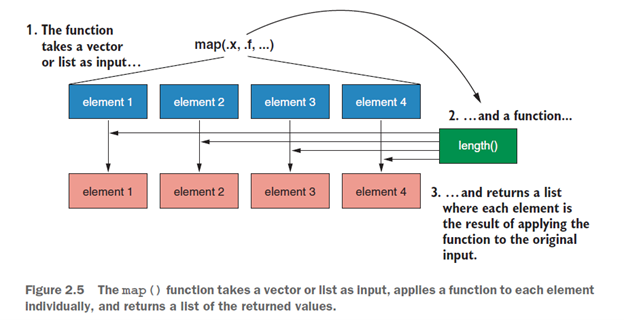
\includegraphics[width=8.67in]{pic}

\begin{Shaded}
\begin{Highlighting}[]
\FunctionTok{map}\NormalTok{(listOfNumerics, length)}
\end{Highlighting}
\end{Shaded}

\begin{verbatim}
$a
[1] 5

$b
[1] 9

$c
[1] 10
\end{verbatim}

\subsubsection{Returning an atomic vector instead of a
list}\label{returning-an-atomic-vector-instead-of-a-list}

So the map() function always returns a list. But what if, instead of
returning a list, we wanted to return an atomic vector? The purrr
package provides a number of functions to do just that:

\begin{itemize}
\tightlist
\item
  map\_dbl() returns a vector of doubles (decimals).
\item
  map\_chr() returns a character vector.
\item
  map\_int() returns a vector of integers.
\item
  map\_lgl() returns a logical vector.
\end{itemize}

Each of these functions returns an atomic vector of the type specified
by its suffix. In this way, we are forced to think about and
predetermine what type of data our output should be. For example, as
shown in listing 2.18, we can return the lengths of each of our
listOfNumerics list elements just as before, using the map\_int()
function. Just like map(), the map\_int() function applies the length()
function to each element of our list, but it returns the output as a
vector of integers. We can do the same thing using the map\_chr()
function, which coerces the output into a character vector, but the
map\_lgl() function throws an error because it can't coerce the output
into a logical vector.

\begin{Shaded}
\begin{Highlighting}[]
\FunctionTok{map\_int}\NormalTok{(listOfNumerics, length)}
\end{Highlighting}
\end{Shaded}

\begin{verbatim}
 a  b  c 
 5  9 10 
\end{verbatim}

\begin{Shaded}
\begin{Highlighting}[]
\FunctionTok{map\_chr}\NormalTok{(listOfNumerics, length)}
\end{Highlighting}
\end{Shaded}

\begin{verbatim}
   a    b    c 
 "5"  "9" "10" 
\end{verbatim}

Returning a tible with map\_df

\begin{Shaded}
\begin{Highlighting}[]
\FunctionTok{map\_df}\NormalTok{(listOfNumerics, length)}
\end{Highlighting}
\end{Shaded}

\begin{verbatim}
# A tibble: 1 x 3
      a     b     c
  <int> <int> <int>
1     5     9    10
\end{verbatim}

\subsubsection{Using anonymous functions inside the map()
family}\label{using-anonymous-functions-inside-the-map-family}

Sometimes we want to apply a function to each element of a list that we
haven't defined yet. Functions that we define on the fly are called
anonymous functions and can be useful when the function we're applying
isn't going to be used often enough to warrant assigning it to an
object. Using base R, we define an anonymous function by simply calling
the function() function.

Defining an anonymous function with function()

\begin{Shaded}
\begin{Highlighting}[]
\FunctionTok{map}\NormalTok{(listOfNumerics, }\ControlFlowTok{function}\NormalTok{(.) . }\SpecialCharTok{+} \DecValTok{2}\NormalTok{)}
\end{Highlighting}
\end{Shaded}

\begin{verbatim}
$a
[1] 0.04950212 1.36613779 2.43528785 2.04404205 2.89637939

$b
[1] 1.181793 1.276449 1.210291 1.099634 2.702149 1.588183 2.128388 3.202655
[9] 3.278436

$c
 [1] 1.8244268 0.6389115 2.8345976 5.3644738 2.7692818 1.8658525 3.0271645
 [8] 1.6654373 1.5941095 1.9513443
\end{verbatim}

\subsubsection{NOTE}\label{note-1}

Notice the . in the anonymous function. This represents the element that
map() is currently iterating over. The expression after function(.) is
the body of the function. There is nothing wrong with this syntax---it
works perfectly fine---but purrr provides a shorthand for function(.):
the \textasciitilde{} (tilde) symbol. by substituting \textasciitilde{}
for function(.).

\begin{Shaded}
\begin{Highlighting}[]
\FunctionTok{map}\NormalTok{(listOfNumerics, }\SpecialCharTok{\textasciitilde{}}\NormalTok{. }\SpecialCharTok{+} \DecValTok{2}\NormalTok{)}
\end{Highlighting}
\end{Shaded}

\begin{verbatim}
$a
[1] 0.04950212 1.36613779 2.43528785 2.04404205 2.89637939

$b
[1] 1.181793 1.276449 1.210291 1.099634 2.702149 1.588183 2.128388 3.202655
[9] 3.278436

$c
 [1] 1.8244268 0.6389115 2.8345976 5.3644738 2.7692818 1.8658525 3.0271645
 [8] 1.6654373 1.5941095 1.9513443
\end{verbatim}

\subsubsection{Using walk() to produce a function's side
effects}\label{using-walk-to-produce-a-functions-side-effects}

Sometimes we want to iterate over a function for its side effects.
Probably the most common example is when we want to produce a series of
plots. In this situation, we can use the walk() function to apply a
function to each element of a list to produce the function's side
effects. The walk() function also returns the original input data we
pass it, so it's useful for plotting an intermediate step in a series of
piped operations. Here's an example of walk() being used to create a
separate histogram for each element of our list:

\begin{Shaded}
\begin{Highlighting}[]
\FunctionTok{par}\NormalTok{(}\AttributeTok{mfrow =} \FunctionTok{c}\NormalTok{(}\DecValTok{1}\NormalTok{, }\DecValTok{3}\NormalTok{))}
\FunctionTok{walk}\NormalTok{(listOfNumerics, hist)}
\end{Highlighting}
\end{Shaded}

\includegraphics{kNN-Logistic-and-Support-Vector-Machine_files/figure-latex/unnamed-chunk-48-1.pdf}

\subsubsection{NOTE}\label{note-2}

The par(mfrow = c(1, 3)) function call simply splits the plotting device
into two rows and four columns for base plots. But what if we want to
use the name of each list element as the title for its histogram? We can
do this using the iwalk() function, which makes the name or index of
each element available to us. In the function we supply to iwalk(), we
can use .x to reference the list element we're iterating over and .y to
reference its name/index:

\begin{Shaded}
\begin{Highlighting}[]
\FunctionTok{par}\NormalTok{(}\AttributeTok{mfrow =} \FunctionTok{c}\NormalTok{(}\DecValTok{1}\NormalTok{, }\DecValTok{3}\NormalTok{))}
\FunctionTok{iwalk}\NormalTok{(listOfNumerics, }\SpecialCharTok{\textasciitilde{}}\FunctionTok{hist}\NormalTok{(.x, }\AttributeTok{main =}\NormalTok{ .y))}
\end{Highlighting}
\end{Shaded}

\includegraphics{kNN-Logistic-and-Support-Vector-Machine_files/figure-latex/unnamed-chunk-49-1.pdf}

\subsubsection{Iterating over multiple lists
simultaneously}\label{iterating-over-multiple-lists-simultaneously}

Sometimes the data we wish to iterate over isn't contained in a single
list. Imagine that we want to multiply each element in our list by a
different value. We can store these values in a separate list and use
the map2() function to iterate over both lists simultaneously,
multiplying the element in the first list by the element in the second.
This time, instead of referencing our data with ., we specifically
reference the first and second lists using .x and .y, respectively:

\begin{Shaded}
\begin{Highlighting}[]
\NormalTok{multipliers }\OtherTok{\textless{}{-}} \FunctionTok{list}\NormalTok{(}\FloatTok{0.5}\NormalTok{, }\DecValTok{10}\NormalTok{, }\DecValTok{3}\NormalTok{)}
\FunctionTok{map2}\NormalTok{(}\AttributeTok{.x =}\NormalTok{ listOfNumerics, }\AttributeTok{.y =}\NormalTok{ multipliers, }\SpecialCharTok{\textasciitilde{}}\NormalTok{.x }\SpecialCharTok{*}\NormalTok{ .y)}
\end{Highlighting}
\end{Shaded}

\begin{verbatim}
$a
[1] -0.97524894 -0.31693111  0.21764393  0.02202102  0.44818969

$b
[1] -8.182067 -7.235512 -7.897090 -9.003664  7.021495 -4.118167  1.283881
[8] 12.026549 12.784362

$c
 [1] -0.5267195 -4.0832654  2.5037927 10.0934215  2.3078454 -0.4024424
 [7]  3.0814934 -1.0036880 -1.2176714 -0.1459670
\end{verbatim}

Now, imagine that instead of iterating over just two lists, we want to
iterate over three or more. The pmap() function allows us to iterate
over multiple lists simultaneously. I use pmap() when I want to test
multiple combinations of arguments for a function. The rnorm() function
draws a random sample from the normal distribution and has three
arguments: n (the number of samples), mean (the center of the
distribution), and sd (the standard deviation). We can create a list of
values for each and then use pmap() to iterate over each list to run the
function on each combination.

We start by using the expand.grid() function to create a data frame
containing every combination of the input vectors. Because data frames
are really just lists of columns, supplying one to pmap() will iterate a
function over each column in the data frame. Essentially, the function
we ask pmap() to iterate over will be run using the arguments contained
in each row of the data frame. Therefore, pmap() will return eight
different random samples, one corresponding to each combination of
arguments in the data frame. Because the first argument of all map
family functions is the data we wish to iterate over, we can chain them
together using the \%\textgreater\% operator. The following code pipes
the random samples returned by pmap() into the iwalk() function to draw
a separate histogram for each sample, labeled with its index.

\begin{Shaded}
\begin{Highlighting}[]
\NormalTok{arguments }\OtherTok{\textless{}{-}} \FunctionTok{expand.grid}\NormalTok{(}\AttributeTok{n =} \FunctionTok{c}\NormalTok{(}\DecValTok{100}\NormalTok{, }\DecValTok{200}\NormalTok{),}
                         \AttributeTok{mean =} \FunctionTok{c}\NormalTok{(}\DecValTok{1}\NormalTok{, }\DecValTok{10}\NormalTok{),}
                         \AttributeTok{sd =} \FunctionTok{c}\NormalTok{(}\DecValTok{1}\NormalTok{, }\DecValTok{10}\NormalTok{))}
\NormalTok{arguments}
\end{Highlighting}
\end{Shaded}

\begin{verbatim}
    n mean sd
1 100    1  1
2 200    1  1
3 100   10  1
4 200   10  1
5 100    1 10
6 200    1 10
7 100   10 10
8 200   10 10
\end{verbatim}

\begin{Shaded}
\begin{Highlighting}[]
\FunctionTok{par}\NormalTok{(}\AttributeTok{mfrow =} \FunctionTok{c}\NormalTok{(}\DecValTok{2}\NormalTok{, }\DecValTok{4}\NormalTok{))}
\FunctionTok{pmap}\NormalTok{(arguments, rnorm) }\SpecialCharTok{\%\textgreater{}\%}
  \FunctionTok{iwalk}\NormalTok{(}\SpecialCharTok{\textasciitilde{}}\FunctionTok{hist}\NormalTok{(.x, }\AttributeTok{main =} \FunctionTok{paste}\NormalTok{(}\StringTok{"Element"}\NormalTok{, .y)))}
\end{Highlighting}
\end{Shaded}

\includegraphics{kNN-Logistic-and-Support-Vector-Machine_files/figure-latex/unnamed-chunk-52-1.pdf}

Don't worry if you haven't memorized all of the tidyverse functions I
just covered--- we'll be using these tools throughout the book in our
machine learning pipelines. There's also much more we can do with
tidyverse tools than I've covered here, but this will certainly be
enough for you to solve the most common data-manipulation problems
you'll encounter. Now that you're armed with the knowledge of how to use
this book, in the next chapter we'll dive into the theory of machine
learning.

\section{PART 2}\label{part-2}

\subsection{CLASSIFICATION}\label{classification}

\subsubsection{Classification Based on Similarities with k-Nearest
Neighbors
(k-NN)}\label{classification-based-on-similarities-with-k-nearest-neighbors-k-nn}

Now that we've covered some basic machine learning terminology, and your
tidyverse skills are developing, let's finally start learning some
practical machine learning skills. The rest of the book is split into
four parts: \emph{Classification} \emph{Regression} \emph{Dimension
reduction} \emph{Clustering}

This is probably the most important chapter of the entire book. In it,
I'm going to show you how the k-nearest neighbors (kNN) algorithm works,
and we're going to use it to classify potential diabetes patients. In
addition, I'm going to use the kNN algorithm to teach you some essential
concepts in machine learning that we will rely on for the rest of the
book. By the end of this chapter, not only will you understand and be
able to use the kNN algorithm to make classification models, but you
will be able to validate its performance and tune it to improve its
performance as much as possible. Once the model is built, you'll learn
how to pass new, unseen data into it and get the data's predicted
classes (the value of the categorical or grouping variable we are trying
to predict)

\subsubsection{The k-Nearest Neighbours}\label{the-k-nearest-neighbours}

Imagine that you work for a reptile conservation project aiming to count
the numbers of grass snakes, adders, and slow worms in a woodland. Your
job is to build a model that allows you to quickly classify reptiles you
find into one of these three classes. When you find one of these
animals, you only have enough time to rapidly estimate its length and
some measure of how aggressive it is toward you, before it slithers away
(funding is very scarce for your project). A reptile expert helps you
manually classify the observations you've made so far, but you decide to
build a kNN classifier to help you quickly classify future specimens you
come across.

We can describe the kNN algorithm (and other machine learning
algorithms) in terms of two phases: \emph{1 The training phase} \emph{2
The prediction phase}

\subsubsection{Building your First k-NN
Model}\label{building-your-first-k-nn-model}

Imagine that you work in a hospital and are trying to improve the
diagnosis of patients with diabetes. You collect diagnostic data over a
few months from suspected diabetes patients and record whether they were
diagnosed as healthy, chemically diabetic, or overtly diabetic. You
would like to use the kNN algorithm to train a model that can predict
which of these classes a new patient will belong to, so that diagnoses
can be improved. This is a three-class classification problem.

\subsubsection{Load the following important
libraries}\label{load-the-following-important-libraries}

\begin{Shaded}
\begin{Highlighting}[]
\FunctionTok{library}\NormalTok{(mlr)}
\FunctionTok{library}\NormalTok{(tidyverse)}
\end{Highlighting}
\end{Shaded}

\subsubsection{Loading and exploring the diabetes
dataset}\label{loading-and-exploring-the-diabetes-dataset}

Now, let's load some data built into the mclust package, convert it into
a tibble, and explore it a little (recall from chapter 2 that a tibble
is the tidyverse way of storing rectangular data): see listing 3.1. We
have a tibble with 145 cases and 4 variables. The class factor shows
that 76 of the cases were non-diabetic (Normal), 36 were chemically
diabetic (Chemical), and 33 were overtly diabetic (Overt). The other
three variables are continuous measures of the level of blood glucose
and insulin after a glucose tolerance test (glucose and insulin,
respectively), and the steady-state level of blood glucose (sspg).

\begin{Shaded}
\begin{Highlighting}[]
\FunctionTok{data}\NormalTok{(diabetes, }\AttributeTok{package =} \StringTok{"mclust"}\NormalTok{)}
\NormalTok{diabetesTib }\OtherTok{\textless{}{-}} \FunctionTok{as\_tibble}\NormalTok{(diabetes)}
\FunctionTok{head}\NormalTok{(diabetesTib)}
\end{Highlighting}
\end{Shaded}

\begin{verbatim}
# A tibble: 6 x 4
  class  glucose insulin  sspg
  <fct>    <dbl>   <dbl> <dbl>
1 Normal      80     356   124
2 Normal      97     289   117
3 Normal     105     319   143
4 Normal      90     356   199
5 Normal      90     323   240
6 Normal      86     381   157
\end{verbatim}

\begin{Shaded}
\begin{Highlighting}[]
\FunctionTok{summary}\NormalTok{(diabetesTib)}
\end{Highlighting}
\end{Shaded}

\begin{verbatim}
      class       glucose       insulin            sspg      
 Chemical:36   Min.   : 70   Min.   :  45.0   Min.   : 10.0  
 Normal  :76   1st Qu.: 90   1st Qu.: 352.0   1st Qu.:118.0  
 Overt   :33   Median : 97   Median : 403.0   Median :156.0  
               Mean   :122   Mean   : 540.8   Mean   :186.1  
               3rd Qu.:112   3rd Qu.: 558.0   3rd Qu.:221.0  
               Max.   :353   Max.   :1568.0   Max.   :748.0  
\end{verbatim}

\subsubsection{View the first few
observations}\label{view-the-first-few-observations}

\begin{Shaded}
\begin{Highlighting}[]
\FunctionTok{head}\NormalTok{(diabetesTib,}\DecValTok{5}\NormalTok{)}
\end{Highlighting}
\end{Shaded}

\begin{verbatim}
# A tibble: 5 x 4
  class  glucose insulin  sspg
  <fct>    <dbl>   <dbl> <dbl>
1 Normal      80     356   124
2 Normal      97     289   117
3 Normal     105     319   143
4 Normal      90     356   199
5 Normal      90     323   240
\end{verbatim}

To show how these variables are related, they are plotted against each
other in figure 3.5. The code to generate these plots is in listing 3.2.

\begin{Shaded}
\begin{Highlighting}[]
\FunctionTok{ggplot}\NormalTok{(diabetesTib, }\FunctionTok{aes}\NormalTok{(glucose, insulin, }\AttributeTok{col =}\NormalTok{ class)) }\SpecialCharTok{+}
  \FunctionTok{geom\_point}\NormalTok{() }\SpecialCharTok{+}
  \FunctionTok{theme\_bw}\NormalTok{()}
\end{Highlighting}
\end{Shaded}

\includegraphics{kNN-Logistic-and-Support-Vector-Machine_files/figure-latex/unnamed-chunk-56-1.pdf}

\begin{Shaded}
\begin{Highlighting}[]
\FunctionTok{ggplot}\NormalTok{(diabetesTib, }\FunctionTok{aes}\NormalTok{(sspg, insulin, }\AttributeTok{col =}\NormalTok{ class)) }\SpecialCharTok{+}
  \FunctionTok{geom\_point}\NormalTok{() }\SpecialCharTok{+}
  \FunctionTok{theme\_bw}\NormalTok{()}
\end{Highlighting}
\end{Shaded}

\includegraphics{kNN-Logistic-and-Support-Vector-Machine_files/figure-latex/unnamed-chunk-56-2.pdf}

\begin{Shaded}
\begin{Highlighting}[]
\FunctionTok{ggplot}\NormalTok{(diabetesTib, }\FunctionTok{aes}\NormalTok{(sspg, glucose, }\AttributeTok{col =}\NormalTok{ class)) }\SpecialCharTok{+}
  \FunctionTok{geom\_point}\NormalTok{() }\SpecialCharTok{+}
  \FunctionTok{theme\_bw}\NormalTok{()}
\end{Highlighting}
\end{Shaded}

\includegraphics{kNN-Logistic-and-Support-Vector-Machine_files/figure-latex/unnamed-chunk-56-3.pdf}

Looking at the data, we can see there are differences in the continuous
variables among the three classes, so let's build a kNN classifier that
we can use to predict diabetes status from measurements of future
patients.

Our dataset only consists of continuous predictor variables, but often
we may be working with categorical predictor variables too. The kNN
algorithm can't handle categorical variables natively; they need to
first be encoded somehow, or distance metrics other than Euclidean
distance must be used. It's also very important for kNN (and many
machine learning algorithms) to scale the predictor variables by
dividing them by their standard deviation. This preserves the
relationships between the variables, but ensures that variables measured
on larger scales aren't given more importance by the algorithm. In the
current example, if we divided the glucose and insulin variables by
1,000,000, then predictions would rely mostly on the value of the sspg
variable. We don't need to scale the predictors ourselves because, by
default, the kNN algorithm wrapped by the mlr package does this for us.

We understand the problem we're trying to solve (classifying new
patients into one of three classes), and now we need to train the kNN
algorithm to build a model that will solve that problem. Building a
machine learning model with the mlr package has three main stages:

\emph{1 Define the task.} The task consists of the data and what we want
to do with it. In this case, the data is diabetesTib, and we want to
classify the data with the class variable as the target variable.

\emph{2 Define the learner.} The learner is simply the name of the
algorithm we plan to use, along with any additional arguments the
algorithm accepts.

\emph{3 Train the model.} This stage is what it sounds like: you pass
the task to the learner, and the learner generates a model that you can
use to make future predictions.

\subparagraph{TIP}\label{tip}

This may seem unnecessarily cumbersome, but splitting the task, learner,
and model into different stages is very useful. It means we can define a
single task and apply multiple learners to it, or define a single
learner and test it with multiple different tasks.

\subsubsection{Telling mlr what we're trying to achieve: Defining the
task}\label{telling-mlr-what-were-trying-to-achieve-defining-the-task}

Let's begin by defining our task. The components needed to define a task
are

\begin{enumerate}
\def\labelenumi{\arabic{enumi}.}
\tightlist
\item
  The data containing the predictor variables (variables we hope contain
  the information needed to make predictions/solve our problem)
\item
  The target variable we want to predict
\end{enumerate}

For supervised learning, the target variable will be categorical if we
have a classification problem, and continuous if we have a regression
problem. For unsupervised learning, we omit the target variable from our
task definition, as we don't have access to labeled data.

We want to build a classification model, so we use the makeClassifTask()
function to define a classification task. When we build regression and
clustering models in parts 3 and 5 of the book, we'll use makeRegrTask()
and makeClusterTask(), respectively. We supply the name of our tibble as
the data argument and the name of the factor that contains the class
labels as the target argument:

\paragraph{NOTE}\label{note-3}

You may notice a warning message from mlr when you build the task,
stating that your data is not a pure data.frame (it's a tibble). This
isn't a problem, because the function will convert the tibble into a
data.frame for you.

\begin{Shaded}
\begin{Highlighting}[]
\NormalTok{diabetesTask }\OtherTok{\textless{}{-}} \FunctionTok{makeClassifTask}\NormalTok{(}\AttributeTok{data =}\NormalTok{ diabetesTib, }\AttributeTok{target =} \StringTok{"class"}\NormalTok{)}
\NormalTok{diabetesTask}
\end{Highlighting}
\end{Shaded}

\begin{verbatim}
Supervised task: diabetesTib
Type: classif
Target: class
Observations: 145
Features:
   numerics     factors     ordered functionals 
          3           0           0           0 
Missings: FALSE
Has weights: FALSE
Has blocking: FALSE
Has coordinates: FALSE
Classes: 3
Chemical   Normal    Overt 
      36       76       33 
Positive class: NA
\end{verbatim}

Next, let's define our learner. The components needed to define a
learner are as follows: * The class of algorithm we are using:
``classif.'' for classification ``regr.'' for regression ``cluster.''
for clustering ``surv.'' and ``multilabel.'' for predicting survival and
multilabel classification, which I won't discuss

\begin{itemize}
\tightlist
\item
  The algorithm we are using
\item
  Any additional options we may wish to use to control the algorithm
\end{itemize}

As you'll see, the first and second components are combined together in
a single character argument to define which algorithm will be used (for
example, ``classif.knn'').

We use the makeLearner() function to define a learner. The first
argument to the makeLearner() function is the algorithm that we're going
to use to train our model. In this case, we want to use the kNN
algorithm, so we supply ``classif.knn'' as the argument. See how this is
the class (``classif.) joined to the name (knn'') of the algorithm? The
argument par.vals stands for parameter values, which allows us to
specify the number of k-nearest neighbors we want the algorithm to use.
For now, we'll just set this to 2, but we'll discuss how to choose k
soon:

\begin{Shaded}
\begin{Highlighting}[]
\NormalTok{knn }\OtherTok{\textless{}{-}} \FunctionTok{makeLearner}\NormalTok{(}\StringTok{"classif.knn"}\NormalTok{, }\AttributeTok{par.vals =} \FunctionTok{list}\NormalTok{(}\StringTok{"k"} \OtherTok{=} \DecValTok{2}\NormalTok{))}
\end{Highlighting}
\end{Shaded}

\subsubsection{Putting it all together: Training the
model}\label{putting-it-all-together-training-the-model}

Now that we've defined our task and our learner, we can now train our
model. The components needed to train a model are the learner and task
we defined earlier.

This is achieved with the train() function, which takes the learner as
the first argument and the task as its second argument:

\begin{Shaded}
\begin{Highlighting}[]
\NormalTok{knnModel }\OtherTok{\textless{}{-}} \FunctionTok{train}\NormalTok{(knn, diabetesTask)}
\NormalTok{knnModel}\SpecialCharTok{$}\NormalTok{task.desc}
\end{Highlighting}
\end{Shaded}

\begin{verbatim}
$id
[1] "diabetesTib"

$type
[1] "classif"

$target
[1] "class"

$size
[1] 145

$n.feat
   numerics     factors     ordered functionals 
          3           0           0           0 

$has.missings
[1] FALSE

$has.weights
[1] FALSE

$has.blocking
[1] FALSE

$has.coordinates
[1] FALSE

$class.levels
[1] "Chemical" "Normal"   "Overt"   

$positive
[1] NA

$negative
[1] NA

$class.distribution

Chemical   Normal    Overt 
      36       76       33 

attr(,"class")
[1] "ClassifTaskDesc"    "SupervisedTaskDesc" "TaskDesc"          
\end{verbatim}

We have our model, so let's pass the data through it to see how it
performs. The predict() function takes unlabeled data and passes it
through the model to get the predicted classes. The first argument is
the model, and the data being passed to it is given as the newdata
argument:

\begin{Shaded}
\begin{Highlighting}[]
\NormalTok{knnPred }\OtherTok{\textless{}{-}} \FunctionTok{predict}\NormalTok{(knnModel, }\AttributeTok{newdata =}\NormalTok{ diabetesTib)}
\NormalTok{knnPred}
\end{Highlighting}
\end{Shaded}

\begin{verbatim}
Prediction: 145 observations
predict.type: response
threshold: 
time: 0.00
   truth response
1 Normal   Normal
2 Normal   Normal
3 Normal   Normal
4 Normal   Normal
5 Normal   Normal
6 Normal   Normal
... (#rows: 145, #cols: 2)
\end{verbatim}

We can pass these predictions as the first argument of the performance()
function. This function compares the classes predicted by the model to
the true classes, and returns performance metrics of how well the
predicted and true values match each other.

We specify which performance metrics we want the function to return by
supplying them as a list to the measures argument. The two measures I've
asked for are mmce, the mean misclassification error; and acc, or
accuracy. MMCE is simply the proportion of cases classified as a class
other than their true class. Accuracy is the opposite of this: the
proportion of cases that were correctly classified by the model. You can
see that the two sum to 1.00:

\begin{Shaded}
\begin{Highlighting}[]
\FunctionTok{performance}\NormalTok{(knnPred, }\AttributeTok{measures =} \FunctionTok{list}\NormalTok{(mmce, acc))}
\end{Highlighting}
\end{Shaded}

\begin{verbatim}
      mmce        acc 
0.03448276 0.96551724 
\end{verbatim}

So our model is correctly classifying 94.48\% of cases! Does this mean
it will perform well on new, unseen patients? The truth is that we don't
know. Evaluating model performance by asking it to make predictions on
data you used to train it in the first place tells you very little about
how the model will perform when making predictions on completely unseen
data. Therefore, you should never evaluate model performance this way.
Before we discuss why, I want to introduce an important concept called
the bias-variance trade-off.

\subsection{Balancing two sources of model
error:}\label{balancing-two-sources-of-model-error}

\subsubsection{The bias-variance
trade-off}\label{the-bias-variance-trade-off}

This is a problem resulting from over-fitting or under-fitting our
model. Underfitting and overfitting both introduce error and reduce the
generalizability of the model: the ability of the model to generalize to
future, unseen data. They are also opposed to each other: somewhere
between a model that underfits and has bias, and a model that overfits
and has variance, is an optimal model that balances the biasvariance
trade-off.

\subsubsection{Using cross-validation to tell if we're overfitting or
underfitting}\label{using-cross-validation-to-tell-if-were-overfitting-or-underfitting}

This process is called cross-validation (CV), and it is an extremely
important approach in any supervised machine learning pipeline. Once we
have cross-validated our model and are happy with its performance, we
then use all the data we have (including the data in the test set) to
train the final model (because typically, the more data we train our
model with, the less bias it will have).

\subparagraph{There are three common cross-validation
approaches:}\label{there-are-three-common-cross-validation-approaches}

\begin{itemize}
\tightlist
\item
  Holdout cross-validation
\item
  K-fold cross-validation
\item
  Leave-one-out cross-validation
\end{itemize}

\subsubsection{Cross-validating our kNN
model}\label{cross-validating-our-knn-model}

Let's start by reminding ourselves of the task and learner we created
earlier:

\begin{Shaded}
\begin{Highlighting}[]
\NormalTok{diabetesTask }\OtherTok{\textless{}{-}} \FunctionTok{makeClassifTask}\NormalTok{(}\AttributeTok{data =}\NormalTok{ diabetesTib, }\AttributeTok{target =} \StringTok{"class"}\NormalTok{)}
\NormalTok{knn }\OtherTok{\textless{}{-}} \FunctionTok{makeLearner}\NormalTok{(}\StringTok{"classif.knn"}\NormalTok{, }\AttributeTok{par.vals =} \FunctionTok{list}\NormalTok{(}\StringTok{"k"} \OtherTok{=} \DecValTok{2}\NormalTok{))}
\end{Highlighting}
\end{Shaded}

Before we train the final model on all the data, let's cross-validate
the learner. Ordinarily, you would decide on a CV strategy most
appropriate for your data; but for the purposes of demonstration, I'm
going to show you holdout, k-fold, and leave-oneout CV.

\subsubsection{Holdout cross-validation}\label{holdout-cross-validation}

When following this approach, you need to decide what proportion of the
data to use as the test set. The larger the test set is, the smaller
your training set will be. Here's the confusing part: performance
estimation by CV is also subject to error and the biasvariance
trade-off. If your test set is too small, then the estimate of
performance is going to have high variance; but if the training set is
too small, then the estimate of performance is going to have high bias.
A commonly used split is to use two-thirds of the data for training and
the remaining one-third as a test set, but this depends on the number of
cases in the data, among other things.

MAKING A HOLDOUT RESAMPLING DESCRIPTION

The first step when employing any CV in mlr is to make a resampling
description, which is simply a set of instructions for how the data will
be split into test and training sets. The first argument to the
makeResampleDesc() function is the CV method we're going to use: in this
case, ``Holdout''. For holdout CV, we need to tell the function what
proportion of the data will be used as the training set, so we supply
this to the split argument:

\begin{Shaded}
\begin{Highlighting}[]
\NormalTok{holdout }\OtherTok{\textless{}{-}} \FunctionTok{makeResampleDesc}\NormalTok{(}\AttributeTok{method =} \StringTok{"Holdout"}\NormalTok{, }\AttributeTok{split =} \DecValTok{2}\SpecialCharTok{/}\DecValTok{3}\NormalTok{,}
                            \AttributeTok{stratify =} \ConstantTok{TRUE}\NormalTok{)}
\end{Highlighting}
\end{Shaded}

\paragraph{PERFORMING HOLDOUT CV}\label{performing-holdout-cv}

Now that we've defined how we're going to cross-validate our learner, we
can run the CV using the resample() function. We supply the learner and
task that we created, and the resampling method we defined a moment ago,
to the resample() function. We also ask it to give us measures of MMCE
and accuracy:

\begin{Shaded}
\begin{Highlighting}[]
\NormalTok{holdoutCV }\OtherTok{\textless{}{-}} \FunctionTok{resample}\NormalTok{(}\AttributeTok{learner =}\NormalTok{ knn, }\AttributeTok{task =}\NormalTok{ diabetesTask,}
                      \AttributeTok{resampling =}\NormalTok{ holdout, }\AttributeTok{measures =} \FunctionTok{list}\NormalTok{(mmce, acc))}
\end{Highlighting}
\end{Shaded}

Extract the aggr component

\begin{Shaded}
\begin{Highlighting}[]
\NormalTok{holdoutCV}\SpecialCharTok{$}\NormalTok{aggr}
\end{Highlighting}
\end{Shaded}

\begin{verbatim}
mmce.test.mean  acc.test.mean 
     0.1020408      0.8979592 
\end{verbatim}

\subparagraph{You'll notice two things:}\label{youll-notice-two-things}

\emph{The accuracy of the model as estimated by holdout cross-validation
is less than when we evaluated its performance on the data we used to
train the full model. This exemplifies my point earlier that models will
perform better on the data that trained them than on unseen data.}

\emph{Your performance metrics will probably be different than mine. In
fact, run the resample() function over and over again, and you'll get a
very different result each time! The reason for this variance is that
the data is randomly split into the test and training sets. Sometimes
the split is such that the model performs well on the test set;
sometimes the split is such that it performs poorly.}

\paragraph{Calculate the Confusion
Matrix}\label{calculate-the-confusion-matrix}

To get a better idea of which groups are being correctly classified and
which are being misclassified, we can construct a confusion matrix. A
confusion matrix is simply a tabular representation of the true and
predicted class of each case in the test set.

\begin{Shaded}
\begin{Highlighting}[]
\FunctionTok{calculateConfusionMatrix}\NormalTok{(holdoutCV}\SpecialCharTok{$}\NormalTok{pred, }\AttributeTok{relative =} \ConstantTok{TRUE}\NormalTok{)}
\end{Highlighting}
\end{Shaded}

\begin{verbatim}
Relative confusion matrix (normalized by row/column):
          predicted
true       Chemical  Normal    Overt     -err.-   
  Chemical 0.75/0.82 0.08/0.04 0.17/0.17 0.25     
  Normal   0.04/0.09 0.96/0.96 0.00/0.00 0.04     
  Overt    0.09/0.09 0.00/0.00 0.91/0.83 0.09     
  -err.-        0.18      0.04      0.17 0.10     


Absolute confusion matrix:
          predicted
true       Chemical Normal Overt -err.-
  Chemical        9      1     2      3
  Normal          1     25     0      1
  Overt           1      0    10      1
  -err.-          2      1     2      5
\end{verbatim}

The absolute confusion matrix is easier to interpret. The rows show the
true class labels, and the columns show the predicted labels. The
numbers represent the number of cases in every combination of true class
and predicted class. For example, in this matrix, 8 patients were
correctly classified as chemically diabetic, but four were erroneously
classified as healthy. Correctly classified patients are found on the
diagonal of the matrix (where true class == predicted class).

From the relative confusion matrix for example, in this matrix, 67\% of
chemically diabetic patients were correctly classified, while 33\% were
misclassified as healthy.

Confusion matrices help us understand which classes our model classifies
well and which ones it does worse at classifying. For example, based on
this confusion matrix, it looks like our model struggles to distinguish
healthy patients from chemically diabetic ones.

\subsubsection{K-fold cross-validation}\label{k-fold-cross-validation}

In k-fold CV, we randomly split the data into approximately equal-sized
chunks called folds. Then we reserve one of the folds as a test set and
use the remaining data as the training set (just like in holdout). We
pass the test set through the model and make a record of the relevant
performance metrics. Now, we use a different fold of the data as our
test set and do the same thing. We continue until all the folds have
been used once as the test set. We then get an average of the
performance metric as an estimate of model performance.

This approach will typically give a more accurate estimate of model
performance because every case appears in the test set once, and we are
averaging the estimates over many runs. But we can improve this a little
by using repeated k-fold CV, where, after the previous procedure, we
shuffle the data around and perform it again.

\paragraph{PERFORMING K-FOLD CV}\label{performing-k-fold-cv}

We perform k-fold CV in the same way as holdout. This time, when we make
our resampling description, we tell it we're going to use repeated
k-fold cross-validation (``RepCV''), and we tell it how many folds we
want to split the data into. The default number of folds is 10, which is
often a good choice, but I want to show you how you can explicitly
control the splits. Next, we tell the function that we want to repeat
the 10-fold CV 50 times with the reps argument. This gives us 500
performance measures to average across! Again, we ask for the classes to
be stratified among the folds:

\begin{Shaded}
\begin{Highlighting}[]
\NormalTok{kFold }\OtherTok{\textless{}{-}} \FunctionTok{makeResampleDesc}\NormalTok{(}\AttributeTok{method =} \StringTok{"RepCV"}\NormalTok{, }\AttributeTok{folds =} \DecValTok{10}\NormalTok{, }\AttributeTok{reps =} \DecValTok{50}\NormalTok{,}
                          \AttributeTok{stratify =} \ConstantTok{TRUE}\NormalTok{)}
\NormalTok{kFoldCV }\OtherTok{\textless{}{-}} \FunctionTok{resample}\NormalTok{(}\AttributeTok{learner =}\NormalTok{ knn, }\AttributeTok{task =}\NormalTok{ diabetesTask,}
                    \AttributeTok{resampling =}\NormalTok{ kFold, }\AttributeTok{measures =} \FunctionTok{list}\NormalTok{(mmce, acc))}
\end{Highlighting}
\end{Shaded}

\paragraph{Extract the aggr
components}\label{extract-the-aggr-components}

\begin{Shaded}
\begin{Highlighting}[]
\NormalTok{kFoldCV}\SpecialCharTok{$}\NormalTok{aggr}
\end{Highlighting}
\end{Shaded}

\begin{verbatim}
mmce.test.mean  acc.test.mean 
     0.1043523      0.8956477 
\end{verbatim}

The model correctly classified 89.8\% of cases on average---much lower
than when we predicted the data we used to train the model! Rerun the
resample() function a few times, and compare the average accuracy after
each run. The estimate is much more stable than when we repeated holdout
CV.

We're usually only interested in the average performance measures, but
you can access the performance measure from every iteration by running

\begin{Shaded}
\begin{Highlighting}[]
\NormalTok{kFoldCV}\SpecialCharTok{$}\NormalTok{measures.test}
\end{Highlighting}
\end{Shaded}

\begin{verbatim}
    iter       mmce       acc
1      1 0.06666667 0.9333333
2      2 0.06666667 0.9333333
3      3 0.07142857 0.9285714
4      4 0.20000000 0.8000000
5      5 0.21428571 0.7857143
6      6 0.00000000 1.0000000
7      7 0.12500000 0.8750000
8      8 0.26666667 0.7333333
9      9 0.07142857 0.9285714
10    10 0.28571429 0.7142857
11    11 0.13333333 0.8666667
12    12 0.21428571 0.7857143
13    13 0.07142857 0.9285714
14    14 0.13333333 0.8666667
15    15 0.06666667 0.9333333
16    16 0.00000000 1.0000000
17    17 0.06666667 0.9333333
18    18 0.07142857 0.9285714
19    19 0.07142857 0.9285714
20    20 0.20000000 0.8000000
21    21 0.06666667 0.9333333
22    22 0.25000000 0.7500000
23    23 0.00000000 1.0000000
24    24 0.06666667 0.9333333
25    25 0.15384615 0.8461538
26    26 0.00000000 1.0000000
27    27 0.14285714 0.8571429
28    28 0.07692308 0.9230769
29    29 0.12500000 0.8750000
30    30 0.13333333 0.8666667
31    31 0.07142857 0.9285714
32    32 0.06666667 0.9333333
33    33 0.23076923 0.7692308
34    34 0.12500000 0.8750000
35    35 0.07692308 0.9230769
36    36 0.26666667 0.7333333
37    37 0.13333333 0.8666667
38    38 0.20000000 0.8000000
39    39 0.00000000 1.0000000
40    40 0.00000000 1.0000000
41    41 0.12500000 0.8750000
42    42 0.06666667 0.9333333
43    43 0.14285714 0.8571429
44    44 0.33333333 0.6666667
45    45 0.00000000 1.0000000
46    46 0.00000000 1.0000000
47    47 0.14285714 0.8571429
48    48 0.14285714 0.8571429
49    49 0.13333333 0.8666667
50    50 0.07142857 0.9285714
51    51 0.00000000 1.0000000
52    52 0.07692308 0.9230769
53    53 0.06666667 0.9333333
54    54 0.00000000 1.0000000
55    55 0.00000000 1.0000000
56    56 0.14285714 0.8571429
57    57 0.00000000 1.0000000
58    58 0.14285714 0.8571429
59    59 0.18750000 0.8125000
60    60 0.14285714 0.8571429
61    61 0.18750000 0.8125000
62    62 0.06666667 0.9333333
63    63 0.06250000 0.9375000
64    64 0.07142857 0.9285714
65    65 0.21428571 0.7857143
66    66 0.13333333 0.8666667
67    67 0.00000000 1.0000000
68    68 0.00000000 1.0000000
69    69 0.00000000 1.0000000
70    70 0.07692308 0.9230769
71    71 0.00000000 1.0000000
72    72 0.13333333 0.8666667
73    73 0.07142857 0.9285714
74    74 0.06666667 0.9333333
75    75 0.07692308 0.9230769
76    76 0.18750000 0.8125000
77    77 0.14285714 0.8571429
78    78 0.12500000 0.8750000
79    79 0.14285714 0.8571429
80    80 0.07692308 0.9230769
81    81 0.23076923 0.7692308
82    82 0.06666667 0.9333333
83    83 0.13333333 0.8666667
84    84 0.00000000 1.0000000
85    85 0.28571429 0.7142857
86    86 0.06250000 0.9375000
87    87 0.07142857 0.9285714
88    88 0.00000000 1.0000000
89    89 0.00000000 1.0000000
90    90 0.14285714 0.8571429
91    91 0.14285714 0.8571429
92    92 0.07142857 0.9285714
93    93 0.21428571 0.7857143
94    94 0.00000000 1.0000000
95    95 0.20000000 0.8000000
96    96 0.14285714 0.8571429
97    97 0.13333333 0.8666667
98    98 0.07142857 0.9285714
99    99 0.06666667 0.9333333
100  100 0.18750000 0.8125000
101  101 0.07142857 0.9285714
102  102 0.13333333 0.8666667
103  103 0.06666667 0.9333333
104  104 0.00000000 1.0000000
105  105 0.14285714 0.8571429
106  106 0.14285714 0.8571429
107  107 0.28571429 0.7142857
108  108 0.07142857 0.9285714
109  109 0.28571429 0.7142857
110  110 0.06250000 0.9375000
111  111 0.06666667 0.9333333
112  112 0.14285714 0.8571429
113  113 0.21428571 0.7857143
114  114 0.13333333 0.8666667
115  115 0.07692308 0.9230769
116  116 0.00000000 1.0000000
117  117 0.12500000 0.8750000
118  118 0.21428571 0.7857143
119  119 0.07142857 0.9285714
120  120 0.00000000 1.0000000
121  121 0.00000000 1.0000000
122  122 0.00000000 1.0000000
123  123 0.00000000 1.0000000
124  124 0.20000000 0.8000000
125  125 0.07692308 0.9230769
126  126 0.06666667 0.9333333
127  127 0.33333333 0.6666667
128  128 0.20000000 0.8000000
129  129 0.06666667 0.9333333
130  130 0.14285714 0.8571429
131  131 0.00000000 1.0000000
132  132 0.06666667 0.9333333
133  133 0.07142857 0.9285714
134  134 0.14285714 0.8571429
135  135 0.06666667 0.9333333
136  136 0.14285714 0.8571429
137  137 0.21428571 0.7857143
138  138 0.13333333 0.8666667
139  139 0.06666667 0.9333333
140  140 0.06666667 0.9333333
141  141 0.07142857 0.9285714
142  142 0.00000000 1.0000000
143  143 0.14285714 0.8571429
144  144 0.13333333 0.8666667
145  145 0.13333333 0.8666667
146  146 0.15384615 0.8461538
147  147 0.06666667 0.9333333
148  148 0.00000000 1.0000000
149  149 0.18750000 0.8125000
150  150 0.00000000 1.0000000
151  151 0.18750000 0.8125000
152  152 0.18750000 0.8125000
153  153 0.15384615 0.8461538
154  154 0.07142857 0.9285714
155  155 0.07692308 0.9230769
156  156 0.07142857 0.9285714
157  157 0.00000000 1.0000000
158  158 0.00000000 1.0000000
159  159 0.20000000 0.8000000
160  160 0.06666667 0.9333333
161  161 0.14285714 0.8571429
162  162 0.06666667 0.9333333
163  163 0.07692308 0.9230769
164  164 0.13333333 0.8666667
165  165 0.14285714 0.8571429
166  166 0.12500000 0.8750000
167  167 0.07142857 0.9285714
168  168 0.00000000 1.0000000
169  169 0.06666667 0.9333333
170  170 0.13333333 0.8666667
171  171 0.07692308 0.9230769
172  172 0.14285714 0.8571429
173  173 0.13333333 0.8666667
174  174 0.21428571 0.7857143
175  175 0.06666667 0.9333333
176  176 0.14285714 0.8571429
177  177 0.06666667 0.9333333
178  178 0.18750000 0.8125000
179  179 0.07142857 0.9285714
180  180 0.06666667 0.9333333
181  181 0.20000000 0.8000000
182  182 0.07142857 0.9285714
183  183 0.00000000 1.0000000
184  184 0.07142857 0.9285714
185  185 0.00000000 1.0000000
186  186 0.07142857 0.9285714
187  187 0.06666667 0.9333333
188  188 0.14285714 0.8571429
189  189 0.07142857 0.9285714
190  190 0.20000000 0.8000000
191  191 0.07142857 0.9285714
192  192 0.21428571 0.7857143
193  193 0.00000000 1.0000000
194  194 0.20000000 0.8000000
195  195 0.14285714 0.8571429
196  196 0.06666667 0.9333333
197  197 0.00000000 1.0000000
198  198 0.13333333 0.8666667
199  199 0.00000000 1.0000000
200  200 0.06666667 0.9333333
201  201 0.14285714 0.8571429
202  202 0.14285714 0.8571429
203  203 0.07142857 0.9285714
204  204 0.13333333 0.8666667
205  205 0.06666667 0.9333333
206  206 0.07142857 0.9285714
207  207 0.06250000 0.9375000
208  208 0.06666667 0.9333333
209  209 0.14285714 0.8571429
210  210 0.14285714 0.8571429
211  211 0.25000000 0.7500000
212  212 0.12500000 0.8750000
213  213 0.07142857 0.9285714
214  214 0.00000000 1.0000000
215  215 0.00000000 1.0000000
216  216 0.14285714 0.8571429
217  217 0.07142857 0.9285714
218  218 0.13333333 0.8666667
219  219 0.06666667 0.9333333
220  220 0.23076923 0.7692308
221  221 0.15384615 0.8461538
222  222 0.15384615 0.8461538
223  223 0.06666667 0.9333333
224  224 0.12500000 0.8750000
225  225 0.06250000 0.9375000
226  226 0.06666667 0.9333333
227  227 0.00000000 1.0000000
228  228 0.21428571 0.7857143
229  229 0.00000000 1.0000000
230  230 0.13333333 0.8666667
231  231 0.06666667 0.9333333
232  232 0.06666667 0.9333333
233  233 0.21428571 0.7857143
234  234 0.07142857 0.9285714
235  235 0.07142857 0.9285714
236  236 0.14285714 0.8571429
237  237 0.14285714 0.8571429
238  238 0.07142857 0.9285714
239  239 0.06250000 0.9375000
240  240 0.06666667 0.9333333
241  241 0.00000000 1.0000000
242  242 0.12500000 0.8750000
243  243 0.20000000 0.8000000
244  244 0.07142857 0.9285714
245  245 0.12500000 0.8750000
246  246 0.07142857 0.9285714
247  247 0.20000000 0.8000000
248  248 0.07692308 0.9230769
249  249 0.06666667 0.9333333
250  250 0.15384615 0.8461538
251  251 0.13333333 0.8666667
252  252 0.07142857 0.9285714
253  253 0.06250000 0.9375000
254  254 0.21428571 0.7857143
255  255 0.20000000 0.8000000
256  256 0.06666667 0.9333333
257  257 0.07692308 0.9230769
258  258 0.21428571 0.7857143
259  259 0.07142857 0.9285714
260  260 0.00000000 1.0000000
261  261 0.20000000 0.8000000
262  262 0.20000000 0.8000000
263  263 0.00000000 1.0000000
264  264 0.06666667 0.9333333
265  265 0.00000000 1.0000000
266  266 0.00000000 1.0000000
267  267 0.00000000 1.0000000
268  268 0.12500000 0.8750000
269  269 0.14285714 0.8571429
270  270 0.26666667 0.7333333
271  271 0.13333333 0.8666667
272  272 0.13333333 0.8666667
273  273 0.00000000 1.0000000
274  274 0.13333333 0.8666667
275  275 0.00000000 1.0000000
276  276 0.18750000 0.8125000
277  277 0.07692308 0.9230769
278  278 0.28571429 0.7142857
279  279 0.20000000 0.8000000
280  280 0.00000000 1.0000000
281  281 0.21428571 0.7857143
282  282 0.00000000 1.0000000
283  283 0.06666667 0.9333333
284  284 0.06666667 0.9333333
285  285 0.12500000 0.8750000
286  286 0.00000000 1.0000000
287  287 0.00000000 1.0000000
288  288 0.00000000 1.0000000
289  289 0.20000000 0.8000000
290  290 0.13333333 0.8666667
291  291 0.21428571 0.7857143
292  292 0.06250000 0.9375000
293  293 0.00000000 1.0000000
294  294 0.28571429 0.7142857
295  295 0.21428571 0.7857143
296  296 0.00000000 1.0000000
297  297 0.20000000 0.8000000
298  298 0.00000000 1.0000000
299  299 0.00000000 1.0000000
300  300 0.18750000 0.8125000
301  301 0.20000000 0.8000000
302  302 0.13333333 0.8666667
303  303 0.06666667 0.9333333
304  304 0.07692308 0.9230769
305  305 0.07692308 0.9230769
306  306 0.15384615 0.8461538
307  307 0.21428571 0.7857143
308  308 0.06250000 0.9375000
309  309 0.18750000 0.8125000
310  310 0.06666667 0.9333333
311  311 0.00000000 1.0000000
312  312 0.07142857 0.9285714
313  313 0.14285714 0.8571429
314  314 0.06666667 0.9333333
315  315 0.13333333 0.8666667
316  316 0.06250000 0.9375000
317  317 0.23076923 0.7692308
318  318 0.14285714 0.8571429
319  319 0.06666667 0.9333333
320  320 0.06250000 0.9375000
321  321 0.06666667 0.9333333
322  322 0.07142857 0.9285714
323  323 0.15384615 0.8461538
324  324 0.00000000 1.0000000
325  325 0.13333333 0.8666667
326  326 0.00000000 1.0000000
327  327 0.14285714 0.8571429
328  328 0.20000000 0.8000000
329  329 0.21428571 0.7857143
330  330 0.25000000 0.7500000
331  331 0.07142857 0.9285714
332  332 0.21428571 0.7857143
333  333 0.13333333 0.8666667
334  334 0.13333333 0.8666667
335  335 0.06666667 0.9333333
336  336 0.06666667 0.9333333
337  337 0.07142857 0.9285714
338  338 0.00000000 1.0000000
339  339 0.20000000 0.8000000
340  340 0.00000000 1.0000000
341  341 0.23076923 0.7692308
342  342 0.21428571 0.7857143
343  343 0.20000000 0.8000000
344  344 0.00000000 1.0000000
345  345 0.06250000 0.9375000
346  346 0.07142857 0.9285714
347  347 0.06666667 0.9333333
348  348 0.13333333 0.8666667
349  349 0.07142857 0.9285714
350  350 0.07692308 0.9230769
351  351 0.23076923 0.7692308
352  352 0.15384615 0.8461538
353  353 0.13333333 0.8666667
354  354 0.06250000 0.9375000
355  355 0.14285714 0.8571429
356  356 0.00000000 1.0000000
357  357 0.13333333 0.8666667
358  358 0.07142857 0.9285714
359  359 0.00000000 1.0000000
360  360 0.12500000 0.8750000
361  361 0.21428571 0.7857143
362  362 0.14285714 0.8571429
363  363 0.12500000 0.8750000
364  364 0.07692308 0.9230769
365  365 0.00000000 1.0000000
366  366 0.14285714 0.8571429
367  367 0.18750000 0.8125000
368  368 0.14285714 0.8571429
369  369 0.06666667 0.9333333
370  370 0.21428571 0.7857143
371  371 0.20000000 0.8000000
372  372 0.06666667 0.9333333
373  373 0.13333333 0.8666667
374  374 0.07692308 0.9230769
375  375 0.06666667 0.9333333
376  376 0.00000000 1.0000000
377  377 0.00000000 1.0000000
378  378 0.13333333 0.8666667
379  379 0.13333333 0.8666667
380  380 0.07142857 0.9285714
381  381 0.07142857 0.9285714
382  382 0.14285714 0.8571429
383  383 0.06250000 0.9375000
384  384 0.13333333 0.8666667
385  385 0.00000000 1.0000000
386  386 0.00000000 1.0000000
387  387 0.00000000 1.0000000
388  388 0.13333333 0.8666667
389  389 0.07142857 0.9285714
390  390 0.13333333 0.8666667
391  391 0.14285714 0.8571429
392  392 0.13333333 0.8666667
393  393 0.06666667 0.9333333
394  394 0.20000000 0.8000000
395  395 0.06250000 0.9375000
396  396 0.00000000 1.0000000
397  397 0.07142857 0.9285714
398  398 0.00000000 1.0000000
399  399 0.26666667 0.7333333
400  400 0.07142857 0.9285714
401  401 0.06666667 0.9333333
402  402 0.07692308 0.9230769
403  403 0.13333333 0.8666667
404  404 0.06666667 0.9333333
405  405 0.14285714 0.8571429
406  406 0.26666667 0.7333333
407  407 0.00000000 1.0000000
408  408 0.06666667 0.9333333
409  409 0.15384615 0.8461538
410  410 0.07142857 0.9285714
411  411 0.20000000 0.8000000
412  412 0.30769231 0.6923077
413  413 0.13333333 0.8666667
414  414 0.00000000 1.0000000
415  415 0.00000000 1.0000000
416  416 0.20000000 0.8000000
417  417 0.12500000 0.8750000
418  418 0.07692308 0.9230769
419  419 0.06666667 0.9333333
420  420 0.13333333 0.8666667
421  421 0.00000000 1.0000000
422  422 0.13333333 0.8666667
423  423 0.14285714 0.8571429
424  424 0.13333333 0.8666667
425  425 0.21428571 0.7857143
426  426 0.06250000 0.9375000
427  427 0.06666667 0.9333333
428  428 0.07142857 0.9285714
429  429 0.21428571 0.7857143
430  430 0.07142857 0.9285714
431  431 0.14285714 0.8571429
432  432 0.12500000 0.8750000
433  433 0.07692308 0.9230769
434  434 0.14285714 0.8571429
435  435 0.14285714 0.8571429
436  436 0.20000000 0.8000000
437  437 0.07142857 0.9285714
438  438 0.06250000 0.9375000
439  439 0.07142857 0.9285714
440  440 0.06666667 0.9333333
441  441 0.13333333 0.8666667
442  442 0.07692308 0.9230769
443  443 0.14285714 0.8571429
444  444 0.20000000 0.8000000
445  445 0.00000000 1.0000000
446  446 0.07692308 0.9230769
447  447 0.18750000 0.8125000
448  448 0.23076923 0.7692308
449  449 0.00000000 1.0000000
450  450 0.20000000 0.8000000
451  451 0.00000000 1.0000000
452  452 0.12500000 0.8750000
453  453 0.00000000 1.0000000
454  454 0.21428571 0.7857143
455  455 0.06666667 0.9333333
456  456 0.12500000 0.8750000
457  457 0.07142857 0.9285714
458  458 0.00000000 1.0000000
459  459 0.14285714 0.8571429
460  460 0.18750000 0.8125000
461  461 0.06250000 0.9375000
462  462 0.07142857 0.9285714
463  463 0.07692308 0.9230769
464  464 0.06666667 0.9333333
465  465 0.13333333 0.8666667
466  466 0.06250000 0.9375000
467  467 0.14285714 0.8571429
468  468 0.28571429 0.7142857
469  469 0.00000000 1.0000000
470  470 0.06666667 0.9333333
471  471 0.06250000 0.9375000
472  472 0.06666667 0.9333333
473  473 0.13333333 0.8666667
474  474 0.07142857 0.9285714
475  475 0.07692308 0.9230769
476  476 0.07692308 0.9230769
477  477 0.15384615 0.8461538
478  478 0.12500000 0.8750000
479  479 0.07142857 0.9285714
480  480 0.06250000 0.9375000
481  481 0.06666667 0.9333333
482  482 0.15384615 0.8461538
483  483 0.23076923 0.7692308
484  484 0.06666667 0.9333333
485  485 0.06666667 0.9333333
486  486 0.00000000 1.0000000
487  487 0.13333333 0.8666667
488  488 0.00000000 1.0000000
489  489 0.21428571 0.7857143
490  490 0.07142857 0.9285714
491  491 0.07142857 0.9285714
492  492 0.14285714 0.8571429
493  493 0.07142857 0.9285714
494  494 0.13333333 0.8666667
495  495 0.00000000 1.0000000
496  496 0.23076923 0.7692308
497  497 0.13333333 0.8666667
498  498 0.13333333 0.8666667
499  499 0.00000000 1.0000000
500  500 0.00000000 1.0000000
\end{verbatim}

\subsubsection{CHOOSING THE NUMBER OF
REPEATS}\label{choosing-the-number-of-repeats}

Your goal when cross-validating a model is to get as accurate and stable
an estimate of model performance as possible. Broadly speaking, the more
repeats you can do, the more accurate and stable these estimates will
become. At some point, though, having more repeats won't improve the
accuracy or stability of the performance estimate. So how do you decide
how many repeats to perform? A sound approach is to choose a number of
repeats that is computationally reasonable, run the process a few times,
and see if the average performance estimate varies a lot. If not, great.
If it does vary a lot, you should increase the number of repeats.

\subsubsection{Confusion Matrix}\label{confusion-matrix}

Now, let's build the confusion matrix based on the repeated k-fold CV:

\begin{Shaded}
\begin{Highlighting}[]
\FunctionTok{calculateConfusionMatrix}\NormalTok{(kFoldCV}\SpecialCharTok{$}\NormalTok{pred, }\AttributeTok{relative =} \ConstantTok{TRUE}\NormalTok{)}
\end{Highlighting}
\end{Shaded}

\begin{verbatim}
Relative confusion matrix (normalized by row/column):
          predicted
true       Chemical  Normal    Overt     -err.-   
  Chemical 0.81/0.78 0.09/0.04 0.09/0.11 0.18     
  Normal   0.04/0.08 0.96/0.96 0.00/0.00 0.04     
  Overt    0.16/0.14 0.00/0.00 0.84/0.89 0.16     
  -err.-        0.22      0.04      0.11 0.10     


Absolute confusion matrix:
          predicted
true       Chemical Normal Overt -err.-
  Chemical     1467    166   167    333
  Normal        154   3646     0    154
  Overt         271      0  1379    271
  -err.-        425    166   167    758
\end{verbatim}

\subsection{Leave-one-out
cross-validation}\label{leave-one-out-cross-validation}

Leave-one-out CV can be thought of as the extreme of k-fold CV: instead
of breaking the data into folds, we reserve a single observation as a
test case, train the model on the whole of the rest of the data, and
then pass the test case through it and record the relevant performance
metrics. Next, we do the same thing but select a different observation
as the test case. We continue doing this until every observation has
been used once as the test case, where we take the average of the
performance metrics.

Leave-one-out CV is useful for small datasets where splitting it into k
folds would give variable results. It is also computationally less
expensive than repeated, k-fold CV.

\paragraph{NOTE}\label{note-4}

A supervised learning model that has not been cross-validated is
virtually useless, because you have no idea whether the predictions it
makes on new data will be accurate or not.

\subsubsection{PERFORMING LEAVE-ONE-OUT
CV}\label{performing-leave-one-out-cv}

Creating a resampling description for leave-one-out is just as simple as
for holdout and k-fold CV. We specify leave-one-out CV when making the
resample description by supplying LOO as the argument to the method.
Because the test set is only a single case, we obviously can't stratify
with leave-one-out. Also, because each case is used once as the test
set, with all the other data used as the training set, there's no need
to repeat the procedure:

\begin{Shaded}
\begin{Highlighting}[]
\NormalTok{LOO }\OtherTok{\textless{}{-}} \FunctionTok{makeResampleDesc}\NormalTok{(}\AttributeTok{method =} \StringTok{"LOO"}\NormalTok{)}
\end{Highlighting}
\end{Shaded}

Now, let's run the CV and get the average performance measures:

\begin{Shaded}
\begin{Highlighting}[]
\NormalTok{LOOCV }\OtherTok{\textless{}{-}} \FunctionTok{resample}\NormalTok{(}\AttributeTok{learner =}\NormalTok{ knn, }\AttributeTok{task =}\NormalTok{ diabetesTask, }\AttributeTok{resampling =}\NormalTok{ LOO,}
                  \AttributeTok{measures =} \FunctionTok{list}\NormalTok{(mmce, acc))}
\end{Highlighting}
\end{Shaded}

\begin{Shaded}
\begin{Highlighting}[]
\NormalTok{LOOCV}\SpecialCharTok{$}\NormalTok{aggr}
\end{Highlighting}
\end{Shaded}

\begin{verbatim}
mmce.test.mean  acc.test.mean 
     0.1034483      0.8965517 
\end{verbatim}

If you rerun the CV over and over again, you'll find that for this model
and data, the performance estimate is more variable than for k-fold but
less variable than for the holdout we ran earlier.

\paragraph{CALCULATING A CONFUSION
MATRIX}\label{calculating-a-confusion-matrix}

Once again, let's look at the confusion matrix:

\begin{Shaded}
\begin{Highlighting}[]
\FunctionTok{calculateConfusionMatrix}\NormalTok{(LOOCV}\SpecialCharTok{$}\NormalTok{pred, }\AttributeTok{relative =} \ConstantTok{TRUE}\NormalTok{)}
\end{Highlighting}
\end{Shaded}

\begin{verbatim}
Relative confusion matrix (normalized by row/column):
          predicted
true       Chemical  Normal    Overt     -err.-   
  Chemical 0.83/0.77 0.06/0.03 0.11/0.12 0.17     
  Normal   0.07/0.13 0.93/0.97 0.00/0.00 0.07     
  Overt    0.12/0.10 0.00/0.00 0.88/0.88 0.12     
  -err.-        0.23      0.03      0.12 0.10     


Absolute confusion matrix:
          predicted
true       Chemical Normal Overt -err.-
  Chemical       30      2     4      6
  Normal          5     71     0      5
  Overt           4      0    29      4
  -err.-          9      2     4     15
\end{verbatim}

So you now know how to apply three commonly used types of
cross-validation! If we've cross-validated our model and are happy that
it will perform well enough on unseen data, then we would train the
model on all of the data available to us, and use this to make future
predictions. But I think we can still improve our kNN model. Remember
how earlier, we manually choose a value of 2 for k? Well, randomly
picking a value of k isn't very clever, and there are much better ways
we can find the optimal value.

How does changing the value of k impact model performance? Well, values
of k that are too low may start to model noise in the data. For example,
if we set k = 1, then a healthy patient could be misclassified as
chemically diabetic just because a single chemically diabetic patient
with an unusually low insulin level was their nearest neighbor. In this
situation, instead of just modeling the systematic differences between
the classes, we're also modeling the noise and unpredictable variability
in the data. On the other hand, if we set k too high, a large number of
dissimilar patients will be included in the vote, and the model will be
insensitive to local differences in the data. This is, of course, the
bias-variance trade-off we talked about earlier.

\subsubsection{Tuning k to improve the
model}\label{tuning-k-to-improve-the-model}

Let's apply hyperparameter tuning to optimize the value of k for our
model. An approach we could follow would be to build models with
different values of k using our full dataset, pass the data back through
the model, and see which value of k gives us the best performance. This
is bad practice, because there's a large chance we'll get a value of k
that overfits the dataset we tuned it on. So once again, we rely on CV
to help us guard against overfitting. The first thing we need to do is
define a range of values over which mlr will try, when tuning k:

\begin{Shaded}
\begin{Highlighting}[]
\NormalTok{knnParamSpace }\OtherTok{\textless{}{-}} \FunctionTok{makeParamSet}\NormalTok{(}\FunctionTok{makeDiscreteParam}\NormalTok{(}\StringTok{"k"}\NormalTok{, }\AttributeTok{values =} \DecValTok{1}\SpecialCharTok{:}\DecValTok{10}\NormalTok{))}
\end{Highlighting}
\end{Shaded}

Next, we define how we want mlr to search the parameter space. There are
a few options for this, and in later chapters we'll explore others, but
for now we're going to use the grid search method. This is probably the
simplest method: it tries every single value in the parameter space when
looking for the best-performing value. For tuning continuous
hyperparameters, or when we are tuning several hyperparameters at once,
grid search becomes prohibitively expensive, so other methods like
random search are preferred:

\begin{Shaded}
\begin{Highlighting}[]
\NormalTok{gridSearch }\OtherTok{\textless{}{-}} \FunctionTok{makeTuneControlGrid}\NormalTok{()}
\end{Highlighting}
\end{Shaded}

Next, we define how we're going to cross-validate the tuning procedure,
and we're going to use my favorite: repeated k-fold CV. The principle
here is that for every value in the parameter space (integers 1 to 10),
we perform repeated k-fold CV. For each value of k, we take the average
performance measure across all those iterations and compare it with the
average performance measures for all the other values of k we tried.
This will hopefully give us the value of k that performs best:

\begin{Shaded}
\begin{Highlighting}[]
\NormalTok{cvForTuning }\OtherTok{\textless{}{-}} \FunctionTok{makeResampleDesc}\NormalTok{(}\StringTok{"RepCV"}\NormalTok{, }\AttributeTok{folds =} \DecValTok{10}\NormalTok{, }\AttributeTok{reps =} \DecValTok{20}\NormalTok{)}
\end{Highlighting}
\end{Shaded}

Now, we call the tuneParams() function to perform the tuning:

\begin{Shaded}
\begin{Highlighting}[]
\NormalTok{tunedK }\OtherTok{\textless{}{-}} \FunctionTok{tuneParams}\NormalTok{(}\StringTok{"classif.knn"}\NormalTok{, }\AttributeTok{task =}\NormalTok{ diabetesTask,}
                     \AttributeTok{resampling =}\NormalTok{ cvForTuning,}
                     \AttributeTok{par.set =}\NormalTok{ knnParamSpace, }\AttributeTok{control =}\NormalTok{ gridSearch)}
\end{Highlighting}
\end{Shaded}

The first and second arguments are the names of the algorithm and task
we're applying, respectively. We give our CV strategy as the resampling
argument, the hyperparameter space we define as the par.set argument,
and the search procedure to the control argument. If we call our tunedK
object, we get the best-performing value of k, 7, and the average MMCE
value for that value. We can access the best-performing value of k
directlyby selecting the \$x component

\begin{Shaded}
\begin{Highlighting}[]
\NormalTok{tunedK}
\end{Highlighting}
\end{Shaded}

\begin{verbatim}
Tune result:
Op. pars: k=7
mmce.test.mean=0.0771667
\end{verbatim}

\begin{Shaded}
\begin{Highlighting}[]
\NormalTok{tunedK}\SpecialCharTok{$}\NormalTok{x}
\end{Highlighting}
\end{Shaded}

\begin{verbatim}
$k
[1] 7
\end{verbatim}

We can also visualize the tuning process

\begin{Shaded}
\begin{Highlighting}[]
\NormalTok{knnTuningData }\OtherTok{\textless{}{-}} \FunctionTok{generateHyperParsEffectData}\NormalTok{(tunedK)}
\FunctionTok{plotHyperParsEffect}\NormalTok{(knnTuningData, }\AttributeTok{x =} \StringTok{"k"}\NormalTok{, }\AttributeTok{y =} \StringTok{"mmce.test.mean"}\NormalTok{,}
                    \AttributeTok{plot.type =} \StringTok{"line"}\NormalTok{) }\SpecialCharTok{+}
\FunctionTok{theme\_bw}\NormalTok{()}
\end{Highlighting}
\end{Shaded}

\includegraphics{kNN-Logistic-and-Support-Vector-Machine_files/figure-latex/unnamed-chunk-81-1.pdf}

Now we can train our final model, using our tuned value of k:

\begin{Shaded}
\begin{Highlighting}[]
\NormalTok{tunedKnn }\OtherTok{\textless{}{-}} \FunctionTok{setHyperPars}\NormalTok{(}\FunctionTok{makeLearner}\NormalTok{(}\StringTok{"classif.knn"}\NormalTok{),}
                         \AttributeTok{par.vals =}\NormalTok{ tunedK}\SpecialCharTok{$}\NormalTok{x)}
\NormalTok{tunedKnnModel }\OtherTok{\textless{}{-}} \FunctionTok{train}\NormalTok{(tunedKnn, diabetesTask)}
\NormalTok{tunedKnnModel}
\end{Highlighting}
\end{Shaded}

\begin{verbatim}
Model for learner.id=classif.knn; learner.class=classif.knn
Trained on: task.id = diabetesTib; obs = 145; features = 3
Hyperparameters: k=7
\end{verbatim}

This is as simple as wrapping the makeLearner() function, where we make
a new kNN learner, inside the setHyperPars() function, and providing the
tuned value of k as the par.vals argument. We then train our final model
as before, using the train() function.

\subsection{Including hyperparameter tuning in
cross-validation}\label{including-hyperparameter-tuning-in-cross-validation}

It validates our entire model-building procedure, including the
hyperparameter-tuning step. The cross-validated performance estimate we
get from this procedure should be a good representation of how we expect
our model to perform on completely new, unseen data. The process looks
pretty complicated, but it is extremely easy to perform with mlr. First,
we define how we're going to perform the inner and outer CV:

\begin{Shaded}
\begin{Highlighting}[]
\NormalTok{inner }\OtherTok{\textless{}{-}} \FunctionTok{makeResampleDesc}\NormalTok{(}\StringTok{"CV"}\NormalTok{)}
\NormalTok{outer }\OtherTok{\textless{}{-}} \FunctionTok{makeResampleDesc}\NormalTok{(}\StringTok{"RepCV"}\NormalTok{, }\AttributeTok{folds =} \DecValTok{10}\NormalTok{, }\AttributeTok{reps =} \DecValTok{5}\NormalTok{)}
\end{Highlighting}
\end{Shaded}

I've chosen to perform ordinary k-fold cross-validation for the inner
loop (10 is the default number of folds) and 10-fold CV, repeated 5
times, for the outer loop. Next, we make what's called a wrapper, which
is basically a learner tied to some preprocessing step. In our case,
this is hyperparameter tuning, so we create a tuning wrapper with
makeTuneWrapper():

\begin{Shaded}
\begin{Highlighting}[]
\NormalTok{knnWrapper }\OtherTok{\textless{}{-}} \FunctionTok{makeTuneWrapper}\NormalTok{(}\StringTok{"classif.knn"}\NormalTok{, }\AttributeTok{resampling =}\NormalTok{ inner, }
                              \AttributeTok{par.set =}\NormalTok{ knnParamSpace,}
                              \AttributeTok{control =}\NormalTok{ gridSearch)}
\end{Highlighting}
\end{Shaded}

Here, we supply the algorithm as the first argument and pass our inner
CV procedure as the resampling argument. We supply our hyperparameter
search space as the par.set argument and our gridSearch method as the
control argument (remember that we created these two objects earlier).
This ``wraps'' together the learning algorithm with the hyperparameter
tuning procedure that will be applied inside the inner CV loop. Now that
we've defined our inner and outer CV strategies and our tuning wrapper,
we run the nested CV procedure:

\begin{Shaded}
\begin{Highlighting}[]
\NormalTok{cvWithTuning }\OtherTok{\textless{}{-}} \FunctionTok{resample}\NormalTok{(knnWrapper, diabetesTask, }\AttributeTok{resampling =}\NormalTok{ outer)}
\end{Highlighting}
\end{Shaded}

The first argument is the wrapper we created a moment ago, the second
argument is the name of the task, and we supply our outer CV strategy as
the resampling argument. Now sit back and relax---this could take a
while! Once it finishes, you can print the average MMCE:

\subsubsection{Misclassification Error}\label{misclassification-error}

\begin{Shaded}
\begin{Highlighting}[]
\NormalTok{cvWithTuning}\SpecialCharTok{$}\NormalTok{aggr}
\end{Highlighting}
\end{Shaded}

\begin{verbatim}
mmce.test.mean 
    0.08704762 
\end{verbatim}

\subsubsection{Classification Accuracy}\label{classification-accuracy}

\begin{Shaded}
\begin{Highlighting}[]
\DecValTok{1}\SpecialCharTok{{-}}\NormalTok{cvWithTuning}\SpecialCharTok{$}\NormalTok{aggr}
\end{Highlighting}
\end{Shaded}

\begin{verbatim}
mmce.test.mean 
     0.9129524 
\end{verbatim}

Your MMCE value will probably be a little different than mine due to the
random nature of the validation procedure, but the model is estimated to
correctly classify 91.447\% of cases on unseen data. That's not bad; and
now that we've cross-validated our model properly, we can be confident
we're not overfitting our data.

\subsubsection{Using our model to make
predictions}\label{using-our-model-to-make-predictions}

We have our model, and we're free to use it to classify new patients!
Let's imagine that some new patients come to the clinic:

\begin{Shaded}
\begin{Highlighting}[]
\NormalTok{newDiabetesPatients }\OtherTok{\textless{}{-}} \FunctionTok{tibble}\NormalTok{(}\AttributeTok{glucose =} \FunctionTok{c}\NormalTok{(}\DecValTok{82}\NormalTok{, }\DecValTok{108}\NormalTok{, }\DecValTok{300}\NormalTok{),}
                              \AttributeTok{insulin =} \FunctionTok{c}\NormalTok{(}\DecValTok{361}\NormalTok{, }\DecValTok{288}\NormalTok{, }\DecValTok{1052}\NormalTok{),}
                              \AttributeTok{sspg =} \FunctionTok{c}\NormalTok{(}\DecValTok{200}\NormalTok{, }\DecValTok{186}\NormalTok{, }\DecValTok{135}\NormalTok{))}
\NormalTok{newDiabetesPatients}
\end{Highlighting}
\end{Shaded}

\begin{verbatim}
# A tibble: 3 x 3
  glucose insulin  sspg
    <dbl>   <dbl> <dbl>
1      82     361   200
2     108     288   186
3     300    1052   135
\end{verbatim}

We can pass these patients into our model and get their predicted
diabetes status:

\begin{Shaded}
\begin{Highlighting}[]
\NormalTok{newPatientsPred }\OtherTok{\textless{}{-}} \FunctionTok{predict}\NormalTok{(tunedKnnModel, }
                           \AttributeTok{newdata =}\NormalTok{ newDiabetesPatients)}
\FunctionTok{getPredictionResponse}\NormalTok{(newPatientsPred)}
\end{Highlighting}
\end{Shaded}

\begin{verbatim}
[1] Normal Normal Overt 
Levels: Chemical Normal Overt
\end{verbatim}

Congratulations! Not only have you built your first machine learning
model, but we've covered some reasonably complex theory, too. In the
next chapter, we're going to learn about logistic regression, but first
I want to list the strengths and weaknesses of the k-nearest neighbor
algorithm.

\subsection{Strengths and weaknesses of
kNN}\label{strengths-and-weaknesses-of-knn}

While it often isn't easy to tell which algorithms will perform well for
a given task, here are some strengths and weaknesses that will help you
decide whether kNN will perform well for your task.

\subsubsection{The strengths of the kNN algorithm are as
follows:}\label{the-strengths-of-the-knn-algorithm-are-as-follows}

\begin{itemize}
\tightlist
\item
  The algorithm is very simple to understand.
\item
  There is no computational cost during the learning process; all the
  computation is done during prediction.
\item
  It makes no assumptions about the data, such as how it's distributed.
\end{itemize}

\subsubsection{The weaknesses of the kNN algorithm are
these:}\label{the-weaknesses-of-the-knn-algorithm-are-these}

\begin{itemize}
\tightlist
\item
  It cannot natively handle categorical variables (they must be recoded
  first, or a different distance metric must be used).
\item
  When the training set is large, it can be computationally expensive to
  compute the distance between new data and all the cases in the
  training set.
\item
  The model can't be interpreted in terms of real-world relationships in
  the data.
\item
  Prediction accuracy can be strongly impacted by noisy data and
  outliers.
\item
  In high-dimensional datasets, kNN tends to perform poorly. This is due
  to a phenomenon you'll learn about in chapter 5, called the curse of
  dimensionality.
\end{itemize}

In brief, in high dimensions the distances between the cases start to
look the same, so finding the nearest neighbors becomes difficult.

\subsection{Summary}\label{summary-1}

kNN is a simple supervised learning algorithm that classifies new data
based on the class membership of its nearest k cases in the training
set. To create a machine learning model in mlr, we create a task and a
learner, and then train the model using them. MMCE is the mean
misclassification error, which is the proportion of misclassified cases
in a classification problem. It is the opposite of accuracy. The
bias-variance trade-off is the balance between two types of error in
predictive accuracy. Models with high bias are underfit, and models with
high variance are overfit. Model performance should never be evaluated
on the data used to train it; cross-validation should be used, instead.
Cross-validation is a set of techniques for evaluating model performance
by splitting the data into training and test sets. Three common types of
cross-validation are holdout, where a single split is used; k-fold,
where the data is split into k chunks and the validation performed on
each chunk; and leave-one-out, where the test set is a single case.
Hyperparameters are options that control how machine learning algorithms
learn, which cannot be learned by the algorithm itself. Hyperparameter
tuning is the best way to find optimal hyperparameters. If we perform a
data-dependent preprocessing step, such as hyperparameter tuning, it's
important to incorporate this in our cross-validation strategy, using
nested cross-validation.

\subsection{Classifying based on odds with logistic
regression}\label{classifying-based-on-odds-with-logistic-regression}

\subsubsection{Building your first logistic regression
model}\label{building-your-first-logistic-regression-model}

Imagine that you're a historian interested in the RMS Titanic, which
famously sank in 1912 after colliding with an iceberg. You want to know
whether socioeconomic factors influenced a person's probability of
surviving the disaster. Luckily, such socioeconomic data is publicly
available! Your aim is to build a binomial logistic regression model to
predict whether a passenger would survive the Titanic disaster, based on
data such as their gender and how much they paid for their ticket.
You're also going to interpret the model to decide which variables were
important in influencing the probability of a passenger surviving. Let's
start by loading the mlr and tidyverse packages:

\begin{Shaded}
\begin{Highlighting}[]
\FunctionTok{library}\NormalTok{(mlr)}
\FunctionTok{library}\NormalTok{(tidyverse)}
\FunctionTok{library}\NormalTok{(titanic)}
\end{Highlighting}
\end{Shaded}

\subsubsection{Loading and exploring the Titanic
dataset}\label{loading-and-exploring-the-titanic-dataset}

Now let's load the data, which is built into the titanic package,
convert it into a tibble (with as\_tibble()), and explore it a little.
We have a tibble containing 891 cases and 12 variables of passengers of
the Titanic. Our goal is to train a model that can use the information
in these variables to predict whether a passenger would survive the
disaster.

\subsubsection{Load the data}\label{load-the-data}

\begin{Shaded}
\begin{Highlighting}[]
\FunctionTok{data}\NormalTok{(titanic\_train, }\AttributeTok{package =} \StringTok{"titanic"}\NormalTok{)}
\NormalTok{titanicTib }\OtherTok{\textless{}{-}} \FunctionTok{as\_tibble}\NormalTok{(titanic\_train)}
\FunctionTok{head}\NormalTok{(titanicTib,}\DecValTok{10}\NormalTok{)}
\end{Highlighting}
\end{Shaded}

\begin{verbatim}
# A tibble: 10 x 12
   PassengerId Survived Pclass Name   Sex     Age SibSp Parch Ticket  Fare Cabin
         <int>    <int>  <int> <chr>  <chr> <dbl> <int> <int> <chr>  <dbl> <chr>
 1           1        0      3 Braun~ male     22     1     0 A/5 2~  7.25 ""   
 2           2        1      1 Cumin~ fema~    38     1     0 PC 17~ 71.3  "C85"
 3           3        1      3 Heikk~ fema~    26     0     0 STON/~  7.92 ""   
 4           4        1      1 Futre~ fema~    35     1     0 113803 53.1  "C12~
 5           5        0      3 Allen~ male     35     0     0 373450  8.05 ""   
 6           6        0      3 Moran~ male     NA     0     0 330877  8.46 ""   
 7           7        0      1 McCar~ male     54     0     0 17463  51.9  "E46"
 8           8        0      3 Palss~ male      2     3     1 349909 21.1  ""   
 9           9        1      3 Johns~ fema~    27     0     2 347742 11.1  ""   
10          10        1      2 Nasse~ fema~    14     1     0 237736 30.1  ""   
# i 1 more variable: Embarked <chr>
\end{verbatim}

The tibble contains the following variables:

\emph{PassengerId}---An arbitrary number unique to each passenger
\emph{Survived}---An integer denoting survival (1 = survived, 0 = died)
\emph{Pclass}---Whether the passenger was housed in first, second, or
third class \emph{Name}---A character vector of the passengers' names
\emph{Sex}---A character vector containing ``male'' and ``female''
\emph{Age}---The age of the passenger \emph{SibSp}---The combined number
of siblings and spouses on board \emph{Parch}---The combined number of
parents and children on board \emph{Ticket}---A character vector with
each passenger's ticket number \emph{Fare}---The amount of money each
passenger paid for their ticket \emph{Cabin}---A character vector of
each passenger's cabin number \emph{Embarked}---A character vector of
which port passengers embarked from

\subsubsection{Making the most of the data: Feature engineering and
feature
selection}\label{making-the-most-of-the-data-feature-engineering-and-feature-selection}

Rarely will you be working with a dataset that is ready for modeling
straight away. Typically, we need to perform some cleaning first to
ensure that we get the most from the data. This includes steps such as
converting data to the correct types, correcting mistakes, and removing
irrelevant data. The titanicTib tibble is no exception; we need to clean
it up before we can pass it to the logistic regression algorithm. We'll
perform three tasks: \emph{1 Convert the Survived, Sex, and Pclass
variables into factors.} \emph{2 Create a new variable called FamSize by
adding SibSp and Parch together.} \emph{3 Select the variables we
believe to be of predictive value for our model.}

\begin{Shaded}
\begin{Highlighting}[]
\NormalTok{fctrs }\OtherTok{\textless{}{-}} \FunctionTok{c}\NormalTok{(}\StringTok{"Survived"}\NormalTok{, }\StringTok{"Sex"}\NormalTok{, }\StringTok{"Pclass"}\NormalTok{)}

\NormalTok{titanicClean }\OtherTok{\textless{}{-}}\NormalTok{ titanicTib }\SpecialCharTok{\%\textgreater{}\%}
  \FunctionTok{mutate\_at}\NormalTok{(}\AttributeTok{.vars =}\NormalTok{ fctrs, }\AttributeTok{.funs =}\NormalTok{ factor) }\SpecialCharTok{\%\textgreater{}\%}
  \FunctionTok{mutate}\NormalTok{(}\AttributeTok{FamSize =}\NormalTok{ SibSp }\SpecialCharTok{+}\NormalTok{ Parch) }\SpecialCharTok{\%\textgreater{}\%}
  \FunctionTok{select}\NormalTok{(Survived, Pclass, Sex, Age, Fare, FamSize)}
\FunctionTok{head}\NormalTok{(titanicClean, }\DecValTok{10}\NormalTok{)}
\end{Highlighting}
\end{Shaded}

\begin{verbatim}
# A tibble: 10 x 6
   Survived Pclass Sex      Age  Fare FamSize
   <fct>    <fct>  <fct>  <dbl> <dbl>   <int>
 1 0        3      male      22  7.25       1
 2 1        1      female    38 71.3        1
 3 1        3      female    26  7.92       0
 4 1        1      female    35 53.1        1
 5 0        3      male      35  8.05       0
 6 0        3      male      NA  8.46       0
 7 0        1      male      54 51.9        0
 8 0        3      male       2 21.1        4
 9 1        3      female    27 11.1        2
10 1        2      female    14 30.1        1
\end{verbatim}

\subsubsection{Plotting the data}\label{plotting-the-data}

Now that we've cleaned our data a little, let's plot it to get better
insight into the relationships in the data. Here's a little trick to
simplify plotting multiple variables together using ggplot2. Let's
convert the data into an untidy format, such that each of the predictor
variable names is held in one column, and its values are held in another
column, using the gather() function (refresh your memory of this by
looking at the end of chapter 2).

NOTE

The gather() function will warn that ``attributes are not identical
across measure variables; they will be dropped.'' This is simply warning
you that the variables you are gathering together don't have the same
factor levels. Ordinarily this might mean you've collapsed variables you
didn't mean to, but in this case we can safely ignore the warning.

\subsubsection{Creating an untidy tibble for
plotting}\label{creating-an-untidy-tibble-for-plotting}

\begin{Shaded}
\begin{Highlighting}[]
\NormalTok{titanicUntidy }\OtherTok{\textless{}{-}} \FunctionTok{gather}\NormalTok{(titanicClean, }\AttributeTok{key =} \StringTok{"Variable"}\NormalTok{, }\AttributeTok{value =} \StringTok{"Value"}\NormalTok{,}
                        \SpecialCharTok{{-}}\NormalTok{Survived)}
\NormalTok{titanicUntidy}
\end{Highlighting}
\end{Shaded}

\begin{verbatim}
# A tibble: 4,455 x 3
   Survived Variable Value
   <fct>    <chr>    <chr>
 1 0        Pclass   3    
 2 1        Pclass   1    
 3 1        Pclass   3    
 4 1        Pclass   1    
 5 0        Pclass   3    
 6 0        Pclass   3    
 7 0        Pclass   1    
 8 0        Pclass   3    
 9 1        Pclass   3    
10 1        Pclass   2    
# i 4,445 more rows
\end{verbatim}

We now have an untidy tibble with three columns: one containing the
Survived factor, one containing the names of the predictor variables,
and one containing their values.

NOTE

Note that the value column is a character vector (). This is because it
contains ``male'' and ``female'' from the Sex variable. As a column can
only hold data of a single type, all the numerical data is also
converted into characters. You may be wondering why we're doing this.
Well, it allows us to use ggplot2's faceting system to plot our
different variables together. In listing 4.4, I take the titanicUntidy
tibble, filter for the rows that do not contain the Pclass or Sex
variables (as these are factors, we'll plot them separately), and pipe
this data into a ggplot() call.

In the ggplot() function call, we supply Survived as the x aesthetic and
Value as the y aesthetic (coercing it into a numeric vector with
as.numeric() because it was converted into a character by our gather()
function call earlier). Next---and here's the cool bit---we ask ggplot2
to facet by the Variable column, using the facet\_wrap() function, and
allow the y-axis to vary between the facets. Faceting allows us to draw
subplots of our data, indexed by some faceting variable. Finally, we add
a violin geometric object, which is similar to a box plot but also shows
the density of data along the y-axis.

\begin{Shaded}
\begin{Highlighting}[]
\NormalTok{titanicUntidy }\SpecialCharTok{\%\textgreater{}\%}
  \FunctionTok{filter}\NormalTok{(Variable }\SpecialCharTok{!=} \StringTok{"Pclass"} \SpecialCharTok{\&}\NormalTok{ Variable }\SpecialCharTok{!=} \StringTok{"Sex"}\NormalTok{) }\SpecialCharTok{\%\textgreater{}\%}
  \FunctionTok{ggplot}\NormalTok{(}\FunctionTok{aes}\NormalTok{(Survived, }\FunctionTok{as.numeric}\NormalTok{(Value))) }\SpecialCharTok{+}
  \FunctionTok{facet\_wrap}\NormalTok{(}\SpecialCharTok{\textasciitilde{}}\NormalTok{ Variable, }\AttributeTok{scales =} \StringTok{"free\_y"}\NormalTok{) }\SpecialCharTok{+}
  \FunctionTok{geom\_violin}\NormalTok{(}\AttributeTok{draw\_quantiles =} \FunctionTok{c}\NormalTok{(}\FloatTok{0.25}\NormalTok{, }\FloatTok{0.5}\NormalTok{, }\FloatTok{0.75}\NormalTok{)) }\SpecialCharTok{+}
\FunctionTok{theme\_bw}\NormalTok{()}
\end{Highlighting}
\end{Shaded}

\includegraphics{kNN-Logistic-and-Support-Vector-Machine_files/figure-latex/unnamed-chunk-94-1.pdf}

Can you see how the faceting worked? Rows in the data with different
values of Variable are plotted on different subplots! This is why we
needed to gather the data into an untidy format: so we could supply a
single variable for ggplot2 to facet by.

Now let's do the same thing for the factors in our dataset by filtering
the data for rows that contain only the Pclass and Sex variables. This
time, we want to see what proportion of passengers in each level of the
factors survived. To do so, we plot the factor levels on the x-axis by
supplying Value as the x aesthetic mapping; and we want to use different
colors to denote survival versus non-survival, so we supply Survived as
the fill aesthetic. We facet by Variable as before and add a bar
geometric object with the argument position = ``fill'', which stacks the
data for survivors and non-survivors such that they sum to 1 to show us
the proportion of each. The resulting plot is shown in figure below.

\begin{Shaded}
\begin{Highlighting}[]
\NormalTok{titanicUntidy }\SpecialCharTok{\%\textgreater{}\%}
  \FunctionTok{filter}\NormalTok{(Variable }\SpecialCharTok{==} \StringTok{"Pclass"} \SpecialCharTok{|}\NormalTok{ Variable }\SpecialCharTok{==} \StringTok{"Sex"}\NormalTok{) }\SpecialCharTok{\%\textgreater{}\%}
  \FunctionTok{ggplot}\NormalTok{(}\FunctionTok{aes}\NormalTok{(Value, }\AttributeTok{fill =}\NormalTok{ Survived)) }\SpecialCharTok{+}
  \FunctionTok{facet\_wrap}\NormalTok{(}\SpecialCharTok{\textasciitilde{}}\NormalTok{ Variable, }\AttributeTok{scales =} \StringTok{"free\_x"}\NormalTok{) }\SpecialCharTok{+}
  \FunctionTok{geom\_bar}\NormalTok{(}\AttributeTok{position =} \StringTok{"fill"}\NormalTok{) }\SpecialCharTok{+}
\FunctionTok{theme\_bw}\NormalTok{()}
\end{Highlighting}
\end{Shaded}

\includegraphics{kNN-Logistic-and-Support-Vector-Machine_files/figure-latex/unnamed-chunk-95-1.pdf}

\begin{Shaded}
\begin{Highlighting}[]
\NormalTok{titanicUntidy }\SpecialCharTok{\%\textgreater{}\%}
  \FunctionTok{filter}\NormalTok{(Variable }\SpecialCharTok{==} \StringTok{"Pclass"} \SpecialCharTok{|}\NormalTok{ Variable }\SpecialCharTok{==} \StringTok{"Sex"}\NormalTok{) }\SpecialCharTok{\%\textgreater{}\%}
  \FunctionTok{ggplot}\NormalTok{(}\FunctionTok{aes}\NormalTok{(Value, }\AttributeTok{fill =}\NormalTok{ Survived)) }\SpecialCharTok{+}
  \FunctionTok{facet\_wrap}\NormalTok{(}\SpecialCharTok{\textasciitilde{}}\NormalTok{ Variable, }\AttributeTok{scales =} \StringTok{"free\_x"}\NormalTok{) }\SpecialCharTok{+}
  \FunctionTok{geom\_bar}\NormalTok{(}\AttributeTok{position =} \StringTok{"stack"}\NormalTok{) }\SpecialCharTok{+}
\FunctionTok{theme\_bw}\NormalTok{()}
\end{Highlighting}
\end{Shaded}

\includegraphics{kNN-Logistic-and-Support-Vector-Machine_files/figure-latex/unnamed-chunk-96-1.pdf}

\begin{Shaded}
\begin{Highlighting}[]
\NormalTok{titanicUntidy }\SpecialCharTok{\%\textgreater{}\%}
  \FunctionTok{filter}\NormalTok{(Variable }\SpecialCharTok{==} \StringTok{"Pclass"} \SpecialCharTok{|}\NormalTok{ Variable }\SpecialCharTok{==} \StringTok{"Sex"}\NormalTok{) }\SpecialCharTok{\%\textgreater{}\%}
  \FunctionTok{ggplot}\NormalTok{(}\FunctionTok{aes}\NormalTok{(Value, }\AttributeTok{fill =}\NormalTok{ Survived)) }\SpecialCharTok{+}
  \FunctionTok{facet\_wrap}\NormalTok{(}\SpecialCharTok{\textasciitilde{}}\NormalTok{ Variable, }\AttributeTok{scales =} \StringTok{"free\_x"}\NormalTok{) }\SpecialCharTok{+}
  \FunctionTok{geom\_bar}\NormalTok{(}\AttributeTok{position =} \StringTok{"dodge"}\NormalTok{) }\SpecialCharTok{+}
\FunctionTok{theme\_bw}\NormalTok{()}
\end{Highlighting}
\end{Shaded}

\includegraphics{kNN-Logistic-and-Support-Vector-Machine_files/figure-latex/unnamed-chunk-97-1.pdf}

So it seems like passengers who survived tended to have slightly more
family members on board (perhaps contradicting our hypothesis), although
passengers with very large families on board tended not to survive. Age
doesn't seem to have had an obvious impact on survival, but being female
meant you would be much more likely to survive. Paying more for your
fare increased your probability of survival, as did being in a higher
class (though the two probably correlate).

\subsubsection{Training the model}\label{training-the-model}

Now that we have our cleaned data, let's create a task, learner, and
model with mlr (specifying ``classif.logreg'' to use logistic regression
as our learner). By setting the argument predict.type = ``prob'', the
trained model will output the estimated probabilities of each class when
making predictions on new data, rather than just the predicted class
membership.

\begin{Shaded}
\begin{Highlighting}[]
\NormalTok{titanicTask }\OtherTok{\textless{}{-}} \FunctionTok{makeClassifTask}\NormalTok{(}\AttributeTok{data =}\NormalTok{ titanicClean, }\AttributeTok{target =} \StringTok{"Survived"}\NormalTok{)}
\NormalTok{logReg }\OtherTok{\textless{}{-}} \FunctionTok{makeLearner}\NormalTok{(}\StringTok{"classif.logreg"}\NormalTok{, }\AttributeTok{predict.type =} \StringTok{"prob"}\NormalTok{)}
\CommentTok{\#logRegModel \textless{}{-} train(logReg, titanicTask)}
\end{Highlighting}
\end{Shaded}

Whoops! Something went wrong. What does the error message say? Hmm, it
seems we have some missing data from the Age variable, and the logistic
regression algorithm doesn't know how to handle that. Let's have a look
at this variable. (I'm only displaying the first 60 elements to save
room, but you can print the entire vector.)

\begin{Shaded}
\begin{Highlighting}[]
\NormalTok{titanicClean}\SpecialCharTok{$}\NormalTok{Age[}\DecValTok{1}\SpecialCharTok{:}\DecValTok{60}\NormalTok{]}
\end{Highlighting}
\end{Shaded}

\begin{verbatim}
 [1] 22.0 38.0 26.0 35.0 35.0   NA 54.0  2.0 27.0 14.0  4.0 58.0 20.0 39.0 14.0
[16] 55.0  2.0   NA 31.0   NA 35.0 34.0 15.0 28.0  8.0 38.0   NA 19.0   NA   NA
[31] 40.0   NA   NA 66.0 28.0 42.0   NA 21.0 18.0 14.0 40.0 27.0   NA  3.0 19.0
[46]   NA   NA   NA   NA 18.0  7.0 21.0 49.0 29.0 65.0   NA 21.0 28.5  5.0 11.0
\end{verbatim}

\subsubsection{Check the total number of missing
observations}\label{check-the-total-number-of-missing-observations}

\begin{Shaded}
\begin{Highlighting}[]
\FunctionTok{sum}\NormalTok{(}\FunctionTok{is.na}\NormalTok{(titanicClean}\SpecialCharTok{$}\NormalTok{Age))}
\end{Highlighting}
\end{Shaded}

\begin{verbatim}
[1] 177
\end{verbatim}

Ah, we have lots of NAs (177 in fact!), which is R's way of labeling
missing data.

\subsubsection{Dealing with missing
data}\label{dealing-with-missing-data}

There are two ways to handle missing data: * Simply exclude cases with
missing data from the analysis * Apply an imputation mechanism to fill
in the gaps

The first option may be valid when the ratio of cases with missing
values to complete cases is very small. In that case, omitting cases
with missing data is unlikely to have a large impact on the performance
of our model. It is a simple, if not elegant, solution to the problem.
The second option, missing value imputation, is the process by which we
use some algorithm to estimate what those missing values would have
been, replace the NAs with these estimates, and use this imputed dataset
to train our model. There are many different ways of estimating the
values of missing data, and we'll use more sophisticated ones throughout
the book, but for now, we'll employ mean imputation, where we simply
take the mean of the variable with missing data and replace missing
values with that.

In listing 4.8, I use mlr's impute() function to replace the missing
data. The first argument is the name of the data, and the cols argument
asks us which columns we want to impute and what method we want to
apply. We supply the cols argument as a list of the column names,
separated by commas if we have more than one. Each column listed should
be followed by an = sign and the imputation method (imputeMean() uses
the mean of the variable to replace NAs). I save the imputed data
structure as an object, imp, and use sum(is.na()) to count the number of
missing values from the data.

\begin{Shaded}
\begin{Highlighting}[]
\NormalTok{imp }\OtherTok{\textless{}{-}} \FunctionTok{impute}\NormalTok{(titanicClean, }\AttributeTok{cols =} \FunctionTok{list}\NormalTok{(}\AttributeTok{Age =} \FunctionTok{imputeMean}\NormalTok{()))}
\end{Highlighting}
\end{Shaded}

\subsubsection{Check the missing value from the previous data
set}\label{check-the-missing-value-from-the-previous-data-set}

\begin{Shaded}
\begin{Highlighting}[]
\FunctionTok{sum}\NormalTok{(}\FunctionTok{is.na}\NormalTok{(titanicClean}\SpecialCharTok{$}\NormalTok{Age))}
\end{Highlighting}
\end{Shaded}

\begin{verbatim}
[1] 177
\end{verbatim}

\subsubsection{Check the missing observations from the new
dataset}\label{check-the-missing-observations-from-the-new-dataset}

\begin{Shaded}
\begin{Highlighting}[]
\FunctionTok{sum}\NormalTok{(}\FunctionTok{is.na}\NormalTok{(imp}\SpecialCharTok{$}\NormalTok{data}\SpecialCharTok{$}\NormalTok{Age))}
\end{Highlighting}
\end{Shaded}

\begin{verbatim}
[1] 0
\end{verbatim}

\subsubsection{Training the model (take
two)}\label{training-the-model-take-two}

Okay, we've imputed those pesky missing values with the mean and created
the new object imp. Now let's try again by creating a task using the
imputed data. The imp object contains both the imputed data and a
description for the imputation process we used. To extract the data, we
simply use imp\$data.

\begin{Shaded}
\begin{Highlighting}[]
\NormalTok{titanicTask }\OtherTok{\textless{}{-}} \FunctionTok{makeClassifTask}\NormalTok{(}\AttributeTok{data =}\NormalTok{ imp}\SpecialCharTok{$}\NormalTok{data, }\AttributeTok{target =} \StringTok{"Survived"}\NormalTok{)}
\NormalTok{logRegModel }\OtherTok{\textless{}{-}} \FunctionTok{train}\NormalTok{(logReg, titanicTask)}
\end{Highlighting}
\end{Shaded}

\subsubsection{Cross-validating the logistic regression
model}\label{cross-validating-the-logistic-regression-model}

Remember that when we cross-validate, we should cross-validate our
entire modelbuilding procedure. This should include any data-dependent
preprocessing steps, such as missing value imputation. In chapter 3, we
used a wrapper function to wrap together our learner and our
hyperparameter tuning procedure. This time, we're going to create a
wrapper for our learner and our missing value imputation. The
makeImputeWrapper() function wraps together a learner (given as the
first argument) and an imputation method. Notice how we specify the
imputation method in exactly the same way as for the impute() function
in listing 4.8, by supplying a list of columns and their imputation
method.

\begin{Shaded}
\begin{Highlighting}[]
\NormalTok{logRegWrapper }\OtherTok{\textless{}{-}} \FunctionTok{makeImputeWrapper}\NormalTok{(}\StringTok{"classif.logreg"}\NormalTok{,}
                                   \AttributeTok{cols =} \FunctionTok{list}\NormalTok{(}\AttributeTok{Age =} \FunctionTok{imputeMean}\NormalTok{()))}
\end{Highlighting}
\end{Shaded}

Now let's apply stratified, 10-fold cross-validation, repeated 50 times,
to our wrapped learner.

NOTE

Remember that we first define our resampling method using
make-ResampleDesc() and then use resample() to run the cross-validation.
Because we're supplying our wrapped learner to the resample() function,
for each fold of the cross-validation, the mean of the Age variable in
the training set will be used to impute any missing values.

\begin{Shaded}
\begin{Highlighting}[]
\NormalTok{kFold }\OtherTok{\textless{}{-}} \FunctionTok{makeResampleDesc}\NormalTok{(}\AttributeTok{method =} \StringTok{"RepCV"}\NormalTok{, }\AttributeTok{folds =} \DecValTok{10}\NormalTok{, }\AttributeTok{reps =} \DecValTok{50}\NormalTok{, }
                          \AttributeTok{stratify =} \ConstantTok{TRUE}\NormalTok{)}
\NormalTok{logRegwithImpute }\OtherTok{\textless{}{-}} \FunctionTok{resample}\NormalTok{(logRegWrapper, titanicTask,}
                             \AttributeTok{resampling =}\NormalTok{ kFold,}
                             \AttributeTok{measures =} \FunctionTok{list}\NormalTok{(acc, fpr, fnr))}
\NormalTok{logRegwithImpute}
\end{Highlighting}
\end{Shaded}

\begin{verbatim}
Resample Result
Task: imp$data
Learner: classif.logreg.imputed
Aggr perf: acc.test.mean=0.7963467,fpr.test.mean=0.2989109,fnr.test.mean=0.1442855
Runtime: 10.0318
\end{verbatim}

As this is a two-class classification problem, we have access to a few
extra performance metrics, such as the false positive rate (fpr) and
false negative rate (fnr). In the crossvalidation procedure in listing
4.11, we ask for accuracy, false positive rate, and false negative rate
to be reported as performance metrics. We can see that although on
average across the repeats our model correctly classified 79.6\% of
passengers, it incorrectly classified 29.9\% of passengers who died as
having survived (false positives), and incorrectly classified 14.4\% of
passengers who survived as having died (false negatives).

\subsubsection{Accuracy is the most important performance metric,
right?}\label{accuracy-is-the-most-important-performance-metric-right}

You might think that the accuracy of a model's predictions is the
defining metric of its performance. Often, this is the case, but
sometimes, it's not. Imagine that you work for a bank as a data
scientist in the fraud-detection department. It's your job to build a
model that predicts whether credit card transactions are legitimate or
fraudulent. Let's say that out of 100,000 credit card transactions, only
1 is fraudulent. Because fraud is relatively rare, (and because they're
serving pizza for lunch today), you decide to build a model that simply
classifies all transactions as legitimate. The model accuracy is
99.999\%. Pretty good? Of course not! The model isn't able to identify
any fraudulent transactions and has a false negative rate of 100\%! The
lesson here is that you should evaluate model performance in the context
of your particular problem. Another example could be building a model
that will guide doctors to use an unpleasant treatment, or not, for a
patient. In the context of this problem, it may be acceptable to
incorrectly not give a patient the unpleasant treatment, but it is
imperative that you don't incorrectly give a patient the treatment if
they don't need it! If positive events are rare (as in our fraudulent
credit card example), or if it is particularly important that you don't
misclassify positive cases as negative, you should favor models that
have a low false negative rate. If negative events are rare, or if it is
particularly important that you don't misclassify negative cases as
positive (as in our medical treatment example), you should favor models
that have a low false positive rate. Take a look at
\url{https://mlr.mlr-org.com/articles/tutorial/measures.html} to see all
the performance measures currently wrapped by mlr and the situations in
which they can be used.

\subsection{Interpreting the model: The odds
ratio}\label{interpreting-the-model-the-odds-ratio}

I mentioned at the start of the chapter that logistic regression is very
popular because of how interpretable the model parameters (the
y-intercept, and the slopes for each of the predictors) are. To extract
the model parameters, we must first turn our mlr model object,
logRegModel, into an R model object using the getLearnerModel()
function. Next, we pass this R model object as the argument to the
coef() function, which stands for coefficients (another term for
parameters), so this function returns the model parameters.

\begin{Shaded}
\begin{Highlighting}[]
\NormalTok{logRegModelData }\OtherTok{\textless{}{-}} \FunctionTok{getLearnerModel}\NormalTok{(logRegModel)}
\FunctionTok{coef}\NormalTok{(logRegModelData)}
\end{Highlighting}
\end{Shaded}

\begin{verbatim}
 (Intercept)      Pclass2      Pclass3      Sexmale          Age         Fare 
 3.809661697 -1.000344806 -2.132428850 -2.775928255 -0.038822458  0.003218432 
     FamSize 
-0.243029114 
\end{verbatim}

The intercept is the log odds of surviving the Titanic disaster when all
continuous variables are 0 and the factors are at their reference
levels. We tend to be more interested in the slopes than the
y-intercept, but these values are in log odds units, which are difficult
to interpret. Instead, people commonly convert them into odds ratios. An
odds ratio is, well, a ratio of odds. For example, if the odds of
surviving the Titanic if you're female are about 7 to 10, and the odds
of surviving if you're male are 2 to 10, then the odds ratio for
surviving if you're female is 3.5. In other words, if you were female,
you would have been 3.5 times more likely to survive than if you were
male. Odds ratios are a very popular way of interpreting the impact of
predictors on an outcome, because they are easily understood.

\subsubsection{Converting model parameters into odds
ratios}\label{converting-model-parameters-into-odds-ratios}

How do we get from log odds to odds ratios? By taking their exponent
(e\^{}log\_odds). We can also calculate 95\% confidence intervals using
the confint() function, to help us decide how strong the evidence is
that each variable has predictive value.

\begin{Shaded}
\begin{Highlighting}[]
\FunctionTok{exp}\NormalTok{(}\FunctionTok{cbind}\NormalTok{(}\AttributeTok{Odds\_Ratio =} \FunctionTok{coef}\NormalTok{(logRegModelData), }\FunctionTok{confint}\NormalTok{(logRegModelData)))}
\end{Highlighting}
\end{Shaded}

\begin{verbatim}
             Odds_Ratio       2.5 %       97.5 %
(Intercept) 45.13516691 19.14718874 109.72483921
Pclass2      0.36775262  0.20650392   0.65220841
Pclass3      0.11854901  0.06700311   0.20885220
Sexmale      0.06229163  0.04182164   0.09116657
Age          0.96192148  0.94700049   0.97652950
Fare         1.00322362  0.99872001   1.00863263
FamSize      0.78424868  0.68315465   0.89110044
\end{verbatim}

Most of these odds ratios are less than 1. An odds ratio less than 1
means an event is less likely to occur. It's usually easier to interpret
these if you divide 1 by them. For example, the odds ratio for surviving
if you were male is 0.06, and 1 divided by 0.06 = 16.7. This means that,
holding all other variables constant, men were 16.7 times less likely to
survive than women. For continuous variables, we interpret the odds
ratio as how much more likely a passenger is to survive for every
one-unit increase in the variable. For example, for every additional
family member, a passenger was 1/0.78 = 1.28 times less likely to
survive. For factors, we interpret the odds ratio as how much more
likely a passenger is to survive, compared to the reference level for
that variable. For example, we have odds ratios for Pclass2 and Pclass3,
which are how many more times passengers in classes 2 and 3 are likely
to survive compared to those in class 1, respectively. The 95\%
confidence intervals indicate the strength of the evidence that each
variable has predictive value. An odds ratio of 1 means the odds are
equal and the variable has no impact on prediction. Therefore, if the
95\% confidence intervals include the value 1, such as those for the
Fare variable, then this may suggest that this variable isn't
contributing anything.

\subsubsection{When a one-unit increase doesn't make
sense}\label{when-a-one-unit-increase-doesnt-make-sense}

A one-unit increase often isn't easily interpretable. Say you get an
odds ratio that says for every additional ant in an anthill, that
anthill is 1.000005 times more likely to survive a termite attack. How
can you comprehend the importance of such a small odds ratio? When it
doesn't make sense to think in one-unit increases, a popular technique
is to log2 transform the continuous variables instead, before training
the model with them. This won't impact the predictions made by the
model, but now the odds ratio can be interpreted this way: every time
the number of ants doubles, the anthill is x times more likely to
survive. This will give much larger and much more interpretable odds
ratios.

\subsubsection{4.5 Using our model to make
predictions}\label{using-our-model-to-make-predictions-1}

We've built, cross-validated, and interpreted our model, and now it
would be nice to use the model to make predictions on new data. This
scenario is a little unusual in that we've built a model based on a
historical event, so (hopefully!) we won't be using it to predict
survival of another Titanic disaster. Nevertheless, I want to illustrate
to you how to make predictions with a logistic regression model, the
same as you can for any other supervised algorithm. Let's load some
unlabeled passenger data, clean it ready for prediction, and pass it
through our model.

\begin{Shaded}
\begin{Highlighting}[]
\FunctionTok{data}\NormalTok{(titanic\_test, }\AttributeTok{package =} \StringTok{"titanic"}\NormalTok{)}
\NormalTok{titanicNew }\OtherTok{\textless{}{-}} \FunctionTok{as\_tibble}\NormalTok{(titanic\_test)}
\NormalTok{titanicNewClean }\OtherTok{\textless{}{-}}\NormalTok{ titanicNew }\SpecialCharTok{\%\textgreater{}\%}
  \FunctionTok{mutate\_at}\NormalTok{(}\AttributeTok{.vars =} \FunctionTok{c}\NormalTok{(}\StringTok{"Sex"}\NormalTok{, }\StringTok{"Pclass"}\NormalTok{), }\AttributeTok{.funs =}\NormalTok{ factor) }\SpecialCharTok{\%\textgreater{}\%}
  \FunctionTok{mutate}\NormalTok{(}\AttributeTok{FamSize =}\NormalTok{ SibSp }\SpecialCharTok{+}\NormalTok{ Parch) }\SpecialCharTok{\%\textgreater{}\%}
  \FunctionTok{select}\NormalTok{(Pclass, Sex, Age, Fare, FamSize)}
\FunctionTok{predict}\NormalTok{(logRegModel, }\AttributeTok{newdata =}\NormalTok{ titanicNewClean)}
\end{Highlighting}
\end{Shaded}

\begin{verbatim}
Prediction: 418 observations
predict.type: prob
threshold: 0=0.50,1=0.50
time: 0.00
     prob.0     prob.1 response
1 0.9178036 0.08219636        0
2 0.5909570 0.40904305        0
3 0.9123303 0.08766974        0
4 0.8927383 0.10726167        0
5 0.4069407 0.59305933        1
6 0.8337609 0.16623907        0
... (#rows: 418, #cols: 3)
\end{verbatim}

\subsection{Strengths and weaknesses of logistic
regression}\label{strengths-and-weaknesses-of-logistic-regression}

While it often isn't easy to tell which algorithms will perform well for
a given task, here are some strengths and weaknesses that will help you
decide whether logistic regression will perform well for you.

\subsubsection{The strengths of the logistic regression algorithm are as
follows:}\label{the-strengths-of-the-logistic-regression-algorithm-are-as-follows}

\begin{itemize}
\tightlist
\item
  It can handle both continuous and categorical predictors.
\item
  The model parameters are very interpretable.
\item
  Predictor variables are not assumed to be normally distributed.
\end{itemize}

\subsubsection{The weaknesses of the logistic regression algorithm are
these:}\label{the-weaknesses-of-the-logistic-regression-algorithm-are-these}

\begin{itemize}
\tightlist
\item
  It won't work when there is complete separation between classes.
\item
  It assumes that the classes are linearly separable. In other words, it
  assumes that a flat surface in n-dimensional space (where n is the
  number of predictors) can be used to separate the classes. If a curved
  surface is required to separate the classes, logistic regression will
  underperform compared to some other algorithms.
\item
  It assumes a linear relationship between each predictor and the log
  odds. If, for example, cases with low and high values of a predictor
  belong to one class, but cases with medium values of the predictor
  belong to another class, this linearity will break down.
\end{itemize}

\subsection{Summary}\label{summary-2}

Logistic regression is a supervised learning algorithm that classifies
new data by calculating the probabilities of the data belonging to each
class. Logistic regression can handle continuous and categorical
predictors, and models a linear relationship between the predictors and
the log odds of belonging to the positive class. Feature engineering is
the process by which we extract information from, or create new
variables from, existing variables to maximize their predictive value.
Feature selection is the process of choosing which variables in a
dataset have predictive value for machine learning models. Imputation is
a strategy for dealing with missing data, where some algorithm is used
to estimate what the missing values would have been. You learned how to
apply mean imputation for the Titanic dataset. Odds ratios are an
informative way of interpreting the impact each of our predictors has on
the odds of a case belonging to the positive class. They can be
calculated by taking the exponent of the model slopes (e\^{}log odds).

\subsection{Classifying by maximizing separation with discriminant
analysis}\label{classifying-by-maximizing-separation-with-discriminant-analysis}

\subsubsection{This chapter covers}\label{this-chapter-covers}

\begin{itemize}
\tightlist
\item
  Understanding linear and quadratic discriminant analysis
\item
  Building discriminant analysis classifiers to predict wines
\end{itemize}

Discriminant analysis is an umbrella term for multiple algorithms that
solve classification problems (where we wish to predict a categorical
variable) in a similar way. While there are various discriminant
analysis algorithms that learn slightly differently, they all find a new
representation of the original data that maximizes the separation
between the classes. Recall from chapter 1 that predictor variables are
the variables we hope contain the information needed to make predictions
on new data. Discriminant function analysis algorithms find a new
representation of the predictor variables (which must be continuous) by
combining them together into new variables that best discriminate the
classes. This combination of predictor variables often has the handy
benefit of reducing the number of predictors to a much smaller number.
Because of this, despite discriminant analysis algorithms being
classification algorithms, they are similar to some of the
dimension-reduction algorithms we'll encounter in part 4 of the book.

\subsubsection{NOTE}\label{note-8}

Dimension reduction is the process of learning how the information in a
set of variables can be condensed into a smaller number of variables,
with as little information loss as possible.

\subsubsection{What is discriminant
analysis?}\label{what-is-discriminant-analysis}

In this section, you'll learn why discriminant analysis is useful and
how it works. Imagine that you want to find out if you can predict how
patients will respond to a drug based on their gene expression. You
measure the expression level of 1,000 genes and record whether they
respond positively, negatively, or not at all to the drug (a threeclass
classification problem). A dataset that has as many predictor variables
as this (and it isn't rare to find datasets this large) presents a few
problems:

\begin{itemize}
\tightlist
\item
  The data is very difficult to explore and plot manually.
\item
  There may be many predictor variables that contain no or very little
  predictive information.
\item
  We have the curse of dimensionality to contend with (a problem
  algorithms encounter
\end{itemize}

when trying to learn patterns in high-dimensional data). In our gene
expression example, it would be nearly impossible to plot all 1,000
genes in such a way that we could interpret the similarities/differences
between the classes. Instead, we could use discriminant analysis to take
all that information and condense it into a manageable number of
discriminant functions, each of which is a combination of the original
variables. Put another way, discriminant analysis takes the predictor
variables as input and finds a new, lower-dimensional representation of
those variables that maximizes the separation between the classes.
Therefore, while discriminant analysis is a classification technique, it
employs dimension reduction to achieve its goal.

Discriminant analysis isn't one algorithm but instead comes in many
flavors. I'm going to teach you the two most fundamental and commonly
used algorithms: * Linear discriminant analysis (LDA) * Quadratic
discriminant analysis (QDA)

In the next section, you'll learn how these algorithms work and how they
differ. For now, suffice it to say that LDA and QDA learn linear
(straight-line) and curved decision boundaries between classes,
respectively.

\subsubsection{How does discriminant analysis
learn?}\label{how-does-discriminant-analysis-learn}

I'll start by explaining how LDA works, and then I'll generalize this to
QDA. Imagine that we have two predictor variables we are trying to use
to separate two classes in our data (see figure 5.3). LDA aims to learn
a new representation of the data that separates the centroid of each
class, while keeping the within-class variance as low as possible. A
centroid is simply the point in the feature space that is the mean of
all the predictors (a vector of means, one for each dimension). Then LDA
finds a line through the origin that, when the data is projected onto
it, simultaneously does the following:

\begin{itemize}
\tightlist
\item
  Maximizes the difference between the class centroids along the line
\item
  Minimizes the within-class variance along the line
\end{itemize}

\subsubsection{Linear discriminant analysis vs.~principal component
analysis}\label{linear-discriminant-analysis-vs.-principal-component-analysis}

If you've come across principal component analysis (PCA) before, you
might be wondering how it differs from linear discriminant analysis
(LDA). PCA is an unsupervised learning algorithm for dimension
reduction, meaning that, unlike LDA, it doesn't rely on labeled data.
While both algorithms can be used to reduce the dimensionality of the
dataset, they do so in different ways and to achieve different goals.
Whereas LDA creates new axes that maximize class separation, so that we
can classify new data using these new axes, PCA creates new axes that
maximize the variance of the data projected onto them. Rather than
classification, the goal of PCA is to explain as much of the variation
and information in the data as possible, using only a small number of
new axes. This new, lower-dimensional representation can then be fed
into other machine learning algorithms. (If you're unfamiliar with PCA,
don't worry! You'll learn about it in depth in chapter 13.) If you want
to reduce the dimensionality of data with labeled class membership, you
should typically favor LDA over PCA. If you want to reduce the
dimensionality of unlabeled data, you should favor PCA (or one of the
many other dimension-reduction algorithms we'll discuss in part 4 of the
book).

\subsubsection{What if we have more than two
classes?}\label{what-if-we-have-more-than-two-classes}

Discriminant analysis can handle classification problems with more than
two classes. But how does it learn the best axis in this situation?
Instead of trying to maximize the separation between class centroids, it
maximizes the separation between each class centroid and the grand
centroid of the data (the centroid of all the data, ignoring class
membership). This is illustrated in figure 5.5, where we have two
continuous measurements made on cases from three classes. The class
centroids are shown with triangles, and the grand centroid is indicated
by a cross.

\subsubsection{Learning curves instead of straight lines:
QDA}\label{learning-curves-instead-of-straight-lines-qda}

LDA performs well if the data within each class is normally distributed
across all the predictor variables, and the classes have similar
covariances. Covariance simply means how much one variable
increases/decreases when another variable increases/decreases. So LDA
assumes that for each class in the dataset, the predictor variables
covary with each other the same amount. This often isn't the case, and
classes have different covariances. In this situation, QDA tends to
perform better than LDA because it doesn't make this assumption (though
it still assumes the data is normally distributed). Instead of learning
straight lines that separate the classes, QDA learns curved lines. It is
also well suited, therefore,to situations in which classes are best
separated by a nonlinear decision boundary. This is illustrated in
figure 5.7.

In the example on the left in the figure, the two classes are normally
distributed across both variables and have equal covariances. We can see
that the covariances are equal because, for both classes, as variable 1
increases, variable 2 decreases by the same amount. In this situation,
LDA and QDA will find similar DFs, although LDA is slightly less prone
to overfitting than QDA because it is less flexible. In the example on
the right in the figure, the two classes are normally distributed, but
their covariances are different. In this situation, QDA will find a
curved DF that, when the data is projected onto it, will tend to do a
better job of separating the classes than a linear DF.

\subsubsection{How do LDA and QDA make
predictions?}\label{how-do-lda-and-qda-make-predictions}

Whichever method you've chosen, the DFs have been constructed, and
you've reduced your high-dimensional data into a small number of
discriminants. How do LDA and QDA use this information to classify new
observations? They use an extremely important statistical theorem called
Bayes' rule. Bayes' rule provides us with a way of answering the
following question: given then values of the predictor variables for any
case in our data, what is the probability of that case belonging to
class k? This is written as p(k\textbar x), where k represents
membership in class k, and x represents the values of the predictor
variables. We would read this as ``the probability of belonging to class
k, given the data, x.'' This is given by Bayes' rule:

\subsubsection{Building your first linear and quadratic discriminant
models}\label{building-your-first-linear-and-quadratic-discriminant-models}

Now that you know how discriminant analysis works, you're going to build
your first LDA model. If you haven't already, load the mlr and tidyverse
packages:

\begin{Shaded}
\begin{Highlighting}[]
\FunctionTok{library}\NormalTok{(mlr)}
\FunctionTok{library}\NormalTok{(tidyverse)}
\end{Highlighting}
\end{Shaded}

\subsubsection{Loading and exploring the wine
dataset}\label{loading-and-exploring-the-wine-dataset}

In this section, you'll learn how to build and evaluate the performance
of linear and quadratic discriminant analysis models. Imagine that
you're a detective in a murder mystery. A local wine producer, Ronald
Fisher, was poisoned at a dinner party when someone replaced the wine in
the carafe with wine poisoned with arsenic. Three other (rival) wine
producers were at the party and are your prime suspects. If you can
trace the wine to one of those three vineyards, you'll find your
murderer. As luck would have it, you have access to some previous
chemical analysis of the wines from each of the vineyards, and you order
an analysis of the poisoned carafe at the scene of the crime. Your task
is to build a model that will tell you which vineyard the wine with the
arsenic came from and, therefore, the guilty party. Let's load the wine
data built into the HDclassif package (after installing it), convert it
into a tibble, and explore it a little. We have a tibble containing 178
cases and 14 variables of measurements made on various wine bottles.

\subsubsection{Loading and exploring the wine
dataset}\label{loading-and-exploring-the-wine-dataset-1}

\begin{Shaded}
\begin{Highlighting}[]
\DocumentationTok{\#\# install.packages("HDclassif")}
\FunctionTok{data}\NormalTok{(wine, }\AttributeTok{package =} \StringTok{"HDclassif"}\NormalTok{)}
\NormalTok{wineTib }\OtherTok{\textless{}{-}} \FunctionTok{as\_tibble}\NormalTok{(wine)}
\FunctionTok{head}\NormalTok{(wineTib)}
\end{Highlighting}
\end{Shaded}

\begin{verbatim}
# A tibble: 6 x 14
  class    V1    V2    V3    V4    V5    V6    V7    V8    V9   V10   V11   V12
  <int> <dbl> <dbl> <dbl> <dbl> <int> <dbl> <dbl> <dbl> <dbl> <dbl> <dbl> <dbl>
1     1  14.2  1.71  2.43  15.6   127  2.8   3.06  0.28  2.29  5.64  1.04  3.92
2     1  13.2  1.78  2.14  11.2   100  2.65  2.76  0.26  1.28  4.38  1.05  3.4 
3     1  13.2  2.36  2.67  18.6   101  2.8   3.24  0.3   2.81  5.68  1.03  3.17
4     1  14.4  1.95  2.5   16.8   113  3.85  3.49  0.24  2.18  7.8   0.86  3.45
5     1  13.2  2.59  2.87  21     118  2.8   2.69  0.39  1.82  4.32  1.04  2.93
6     1  14.2  1.76  2.45  15.2   112  3.27  3.39  0.34  1.97  6.75  1.05  2.85
# i 1 more variable: V13 <int>
\end{verbatim}

\subsubsection{Check the structure of the
data}\label{check-the-structure-of-the-data}

\begin{Shaded}
\begin{Highlighting}[]
\FunctionTok{str}\NormalTok{(wineTib)}
\end{Highlighting}
\end{Shaded}

\begin{verbatim}
tibble [178 x 14] (S3: tbl_df/tbl/data.frame)
 $ class: int [1:178] 1 1 1 1 1 1 1 1 1 1 ...
 $ V1   : num [1:178] 14.2 13.2 13.2 14.4 13.2 ...
 $ V2   : num [1:178] 1.71 1.78 2.36 1.95 2.59 1.76 1.87 2.15 1.64 1.35 ...
 $ V3   : num [1:178] 2.43 2.14 2.67 2.5 2.87 2.45 2.45 2.61 2.17 2.27 ...
 $ V4   : num [1:178] 15.6 11.2 18.6 16.8 21 15.2 14.6 17.6 14 16 ...
 $ V5   : int [1:178] 127 100 101 113 118 112 96 121 97 98 ...
 $ V6   : num [1:178] 2.8 2.65 2.8 3.85 2.8 3.27 2.5 2.6 2.8 2.98 ...
 $ V7   : num [1:178] 3.06 2.76 3.24 3.49 2.69 3.39 2.52 2.51 2.98 3.15 ...
 $ V8   : num [1:178] 0.28 0.26 0.3 0.24 0.39 0.34 0.3 0.31 0.29 0.22 ...
 $ V9   : num [1:178] 2.29 1.28 2.81 2.18 1.82 1.97 1.98 1.25 1.98 1.85 ...
 $ V10  : num [1:178] 5.64 4.38 5.68 7.8 4.32 6.75 5.25 5.05 5.2 7.22 ...
 $ V11  : num [1:178] 1.04 1.05 1.03 0.86 1.04 1.05 1.02 1.06 1.08 1.01 ...
 $ V12  : num [1:178] 3.92 3.4 3.17 3.45 2.93 2.85 3.58 3.58 2.85 3.55 ...
 $ V13  : int [1:178] 1065 1050 1185 1480 735 1450 1290 1295 1045 1045 ...
\end{verbatim}

Often, as data scientists, we receive data that is messy or not well
curated. In this case, the names of the variables are missing! We could
continue working with V1, V2, and so on, but it would be hard to keep
track of which variable is which. So we're going to manually add the
variable names. Who said the life of a data scientist was glamorous?
Then, we'll convert the class variable to a factor.

\subsubsection{Cleaning the dataset}\label{cleaning-the-dataset}

\begin{Shaded}
\begin{Highlighting}[]
\FunctionTok{names}\NormalTok{(wineTib) }\OtherTok{\textless{}{-}} \FunctionTok{c}\NormalTok{(}\StringTok{"Class"}\NormalTok{, }\StringTok{"Alco"}\NormalTok{, }\StringTok{"Malic"}\NormalTok{, }\StringTok{"Ash"}\NormalTok{, }\StringTok{"Alk"}\NormalTok{, }\StringTok{"Mag"}\NormalTok{,}
                    \StringTok{"Phe"}\NormalTok{, }\StringTok{"Flav"}\NormalTok{, }\StringTok{"Non\_flav"}\NormalTok{, }\StringTok{"Proan"}\NormalTok{, }\StringTok{"Col"}\NormalTok{, }\StringTok{"Hue"}\NormalTok{,}
                    \StringTok{"OD"}\NormalTok{, }\StringTok{"Prol"}\NormalTok{)}
\NormalTok{wineTib}\SpecialCharTok{$}\NormalTok{Class }\OtherTok{\textless{}{-}} \FunctionTok{as.factor}\NormalTok{(wineTib}\SpecialCharTok{$}\NormalTok{Class)}
\NormalTok{wineTib}
\end{Highlighting}
\end{Shaded}

\begin{verbatim}
# A tibble: 178 x 14
   Class  Alco Malic   Ash   Alk   Mag   Phe  Flav Non_flav Proan   Col   Hue
   <fct> <dbl> <dbl> <dbl> <dbl> <int> <dbl> <dbl>    <dbl> <dbl> <dbl> <dbl>
 1 1      14.2  1.71  2.43  15.6   127  2.8   3.06     0.28  2.29  5.64  1.04
 2 1      13.2  1.78  2.14  11.2   100  2.65  2.76     0.26  1.28  4.38  1.05
 3 1      13.2  2.36  2.67  18.6   101  2.8   3.24     0.3   2.81  5.68  1.03
 4 1      14.4  1.95  2.5   16.8   113  3.85  3.49     0.24  2.18  7.8   0.86
 5 1      13.2  2.59  2.87  21     118  2.8   2.69     0.39  1.82  4.32  1.04
 6 1      14.2  1.76  2.45  15.2   112  3.27  3.39     0.34  1.97  6.75  1.05
 7 1      14.4  1.87  2.45  14.6    96  2.5   2.52     0.3   1.98  5.25  1.02
 8 1      14.1  2.15  2.61  17.6   121  2.6   2.51     0.31  1.25  5.05  1.06
 9 1      14.8  1.64  2.17  14      97  2.8   2.98     0.29  1.98  5.2   1.08
10 1      13.9  1.35  2.27  16      98  2.98  3.15     0.22  1.85  7.22  1.01
# i 168 more rows
# i 2 more variables: OD <dbl>, Prol <int>
\end{verbatim}

That's much better. We can see that we have 13 continuous measurements
made on 178 bottles of wine, where each measurement is the amount of a
different compound/element in the wine. We also have a single
categorical variable, Class, which tells us which vineyard the bottle
comes from.

NOTE Lots of people consider it good form to keep variable names
lowercase. I don't mind so much so long as my style is consistent.
Therefore, notice that I changed the name of the grouping variable class
to Class.

\subsubsection{Plotting the data}\label{plotting-the-data-1}

Let's plot the data to get an idea of how the compounds vary between the
vineyards. As for the Titanic dataset in chapter 4, we're going to
gather the data into an untidy format so we can facet by each of the
variables.

\subsubsection{Creating an untidy tibble for
plotting}\label{creating-an-untidy-tibble-for-plotting-1}

\begin{Shaded}
\begin{Highlighting}[]
\NormalTok{wineUntidy }\OtherTok{\textless{}{-}} \FunctionTok{gather}\NormalTok{(wineTib, }\StringTok{"Variable"}\NormalTok{, }\StringTok{"Value"}\NormalTok{, }\SpecialCharTok{{-}}\NormalTok{Class)}
\NormalTok{wineUntidy}
\end{Highlighting}
\end{Shaded}

\begin{verbatim}
# A tibble: 2,314 x 3
   Class Variable Value
   <fct> <chr>    <dbl>
 1 1     Alco      14.2
 2 1     Alco      13.2
 3 1     Alco      13.2
 4 1     Alco      14.4
 5 1     Alco      13.2
 6 1     Alco      14.2
 7 1     Alco      14.4
 8 1     Alco      14.1
 9 1     Alco      14.8
10 1     Alco      13.9
# i 2,304 more rows
\end{verbatim}

\subsubsection{Plot}\label{plot}

\begin{Shaded}
\begin{Highlighting}[]
\FunctionTok{ggplot}\NormalTok{(wineUntidy, }\FunctionTok{aes}\NormalTok{(Class, Value)) }\SpecialCharTok{+}
\FunctionTok{facet\_wrap}\NormalTok{(}\SpecialCharTok{\textasciitilde{}}\NormalTok{ Variable, }\AttributeTok{scales =} \StringTok{"free\_y"}\NormalTok{) }\SpecialCharTok{+}
\FunctionTok{geom\_boxplot}\NormalTok{() }\SpecialCharTok{+}
\FunctionTok{theme\_bw}\NormalTok{()}
\end{Highlighting}
\end{Shaded}

\includegraphics{kNN-Logistic-and-Support-Vector-Machine_files/figure-latex/unnamed-chunk-115-1.pdf}

Box and whiskers plots of each continuous variable in the data against
vineyard number. For the box and whiskers, the thick horizontal line
represents the median, the box represents the interquartile range (IQR),
the whiskers represent the Tukey range (1.5 times the IQR above and
below the quartiles), and the dots represent data outside of the Tukey
range.

A data scientist (and detective working the case) looking at this data
would jump for joy! Look at how many obvious differences there are
between wines from the three different vineyards. We should easily be
able to build a well-performing classification model because the classes
are so separable.

\subsubsection{Training the models}\label{training-the-models}

Let's define our task and learner, and build a model as usual. This
time, we supply ``classif.lda'' as the argument to makeLearner() to
specify that we're going to use LDA.

TIP LDA and QDA have no hyperparameters to tune and are therefore said
to have a closed-form solution. In other words, all the information that
LDA and QDA need is in the data. Their performance is also unaffected by
variables on different scales. They will give the same result whether
the data is scaled or not!

\subsubsection{Creating the task and learner, and training the
model}\label{creating-the-task-and-learner-and-training-the-model}

\begin{Shaded}
\begin{Highlighting}[]
\NormalTok{wineTask }\OtherTok{\textless{}{-}} \FunctionTok{makeClassifTask}\NormalTok{(}\AttributeTok{data =}\NormalTok{ wineTib, }\AttributeTok{target =} \StringTok{"Class"}\NormalTok{)}
\NormalTok{lda }\OtherTok{\textless{}{-}} \FunctionTok{makeLearner}\NormalTok{(}\StringTok{"classif.lda"}\NormalTok{)}
\NormalTok{ldaModel }\OtherTok{\textless{}{-}} \FunctionTok{train}\NormalTok{(lda, wineTask)}
\end{Highlighting}
\end{Shaded}

NOTE Recall from chapter 3 that the makeClassifTask() function warns us
that our data is a tibble and not a pure data.frame. This warning can be
safely ignored.

Let's extract the model information using the getLearnerModel()
function, and get DF values for each case using the predict() function.
By printing head(ldaPreds), we can see that the model has learned two
DFs, LD1 and LD2, and that the predict() function has indeed returned
the values for these functions for each case in our wineTib dataset.

\subsubsection{Extracting DF values for each
case}\label{extracting-df-values-for-each-case}

\begin{Shaded}
\begin{Highlighting}[]
\NormalTok{ldaModelData }\OtherTok{\textless{}{-}} \FunctionTok{getLearnerModel}\NormalTok{(ldaModel)}
\NormalTok{ldaPreds }\OtherTok{\textless{}{-}} \FunctionTok{predict}\NormalTok{(ldaModelData)}\SpecialCharTok{$}\NormalTok{x}
\FunctionTok{head}\NormalTok{(ldaPreds)}
\end{Highlighting}
\end{Shaded}

\begin{verbatim}
        LD1       LD2
1 -4.700244 1.9791383
2 -4.301958 1.1704129
3 -3.420720 1.4291014
4 -4.205754 4.0028715
5 -1.509982 0.4512239
6 -4.518689 3.2131376
\end{verbatim}

To visualize how well these two learned DFs separate the bottles of wine
from the three vineyards, let's plot them against each other. We start
by piping the wineTib dataset into a mutate() call where we create a new
column for each of the DFs. We pipe this mutated tibble into a ggplot()
call and set LD1, LD2, and Class as the x, y, and color aesthetics,
respectively. Finally, we add a geom\_point() layer to add dots, and a
stat\_ellipse() layer to draw 95\% confidence ellipses around each
class.

\begin{Shaded}
\begin{Highlighting}[]
\NormalTok{wineTib }\SpecialCharTok{\%\textgreater{}\%}
  \FunctionTok{mutate}\NormalTok{(}\AttributeTok{LD1 =}\NormalTok{ ldaPreds[, }\DecValTok{1}\NormalTok{],}
         \AttributeTok{LD2 =}\NormalTok{ ldaPreds[, }\DecValTok{2}\NormalTok{]) }\SpecialCharTok{\%\textgreater{}\%}
  \FunctionTok{ggplot}\NormalTok{(}\FunctionTok{aes}\NormalTok{(LD1, LD2, }\AttributeTok{col =}\NormalTok{ Class)) }\SpecialCharTok{+}
  \FunctionTok{geom\_point}\NormalTok{() }\SpecialCharTok{+}
  \FunctionTok{stat\_ellipse}\NormalTok{()}\SpecialCharTok{+}
  \FunctionTok{ggtitle}\NormalTok{(}\StringTok{"A Plot of Linear Discriminant Analysis for Wine Class"}\NormalTok{)}
\end{Highlighting}
\end{Shaded}

\includegraphics{kNN-Logistic-and-Support-Vector-Machine_files/figure-latex/unnamed-chunk-118-1.pdf}

The plot above shows the the DFs plotted against each other. The values
for LD1 and LD2 for each case are plotted against each other, shaded by
their class.

Looking good. Can you see that LDA has reduced our 13 predictor
variables into just two DFs that do an excellent job of separating the
wines from each of the vineyards? Next, let's use exactly the same
procedure to build a QDA model.

\begin{Shaded}
\begin{Highlighting}[]
\NormalTok{qda }\OtherTok{\textless{}{-}} \FunctionTok{makeLearner}\NormalTok{(}\StringTok{"classif.qda"}\NormalTok{)}
\NormalTok{qdaModel }\OtherTok{\textless{}{-}} \FunctionTok{train}\NormalTok{(qda, wineTask)}
\end{Highlighting}
\end{Shaded}

NOTE Sadly, it isn't easy to extract the DFs from the implementation of
QDA that mlr uses, to plot them as we did for LDA. Now, let's
cross-validate our LDA and QDA models together to estimate how they'll
perform on new data.

\subsubsection{Cross validating LDA and
QDA}\label{cross-validating-lda-and-qda}

\begin{Shaded}
\begin{Highlighting}[]
\NormalTok{kFold }\OtherTok{\textless{}{-}} \FunctionTok{makeResampleDesc}\NormalTok{(}\AttributeTok{method =} \StringTok{"RepCV"}\NormalTok{, }\AttributeTok{folds =} \DecValTok{10}\NormalTok{, }\AttributeTok{reps =} \DecValTok{50}\NormalTok{,}
\AttributeTok{stratify =} \ConstantTok{TRUE}\NormalTok{)}
\NormalTok{ldaCV }\OtherTok{\textless{}{-}} \FunctionTok{resample}\NormalTok{(}\AttributeTok{learner =}\NormalTok{ lda, }\AttributeTok{task =}\NormalTok{ wineTask, }\AttributeTok{resampling =}\NormalTok{ kFold,}
                  \AttributeTok{measures =} \FunctionTok{list}\NormalTok{(mmce, acc))}
\NormalTok{qdaCV }\OtherTok{\textless{}{-}} \FunctionTok{resample}\NormalTok{(}\AttributeTok{learner =}\NormalTok{ qda, }\AttributeTok{task =}\NormalTok{ wineTask, }\AttributeTok{resampling =}\NormalTok{ kFold,}
                  \AttributeTok{measures =} \FunctionTok{list}\NormalTok{(mmce, acc))}
\end{Highlighting}
\end{Shaded}

\subsubsection{Extract the Performance
Metric}\label{extract-the-performance-metric}

\begin{Shaded}
\begin{Highlighting}[]
\NormalTok{ldaCV}\SpecialCharTok{$}\NormalTok{aggr}
\end{Highlighting}
\end{Shaded}

\begin{verbatim}
mmce.test.mean  acc.test.mean 
    0.01226952     0.98773048 
\end{verbatim}

\begin{Shaded}
\begin{Highlighting}[]
\NormalTok{qdaCV}\SpecialCharTok{$}\NormalTok{aggr}
\end{Highlighting}
\end{Shaded}

\begin{verbatim}
mmce.test.mean  acc.test.mean 
   0.008498366    0.991501634 
\end{verbatim}

Great! Our LDA model correctly classified 98.8\% of wine bottles on
average. There isn't much room for improvement here, but our QDA model
managed to correctly classify 99.2\% of cases! Let's also look at the
confusion matrices (interpreting them is part of the chapter's
exercises):

\begin{Shaded}
\begin{Highlighting}[]
\FunctionTok{calculateConfusionMatrix}\NormalTok{(ldaCV}\SpecialCharTok{$}\NormalTok{pred, }\AttributeTok{relative =} \ConstantTok{TRUE}\NormalTok{)}
\end{Highlighting}
\end{Shaded}

\begin{verbatim}
Relative confusion matrix (normalized by row/column):
        predicted
true     1           2           3           -err.-     
  1      1e+00/1e+00 7e-04/6e-04 0e+00/0e+00 7e-04      
  2      1e-02/1e-02 1e+00/1e+00 1e-02/2e-02 3e-02      
  3      0e+00/0e+00 7e-03/5e-03 1e+00/1e+00 7e-03      
  -err.-       0.013       0.005       0.022 0.01       


Absolute confusion matrix:
        predicted
true        1    2    3 -err.-
  1      2948    2    0      2
  2        38 3459   53     91
  3         0   16 2384     16
  -err.-   38   18   53    109
\end{verbatim}

\begin{Shaded}
\begin{Highlighting}[]
\FunctionTok{calculateConfusionMatrix}\NormalTok{(qdaCV}\SpecialCharTok{$}\NormalTok{pred, }\AttributeTok{relative =} \ConstantTok{TRUE}\NormalTok{)}
\end{Highlighting}
\end{Shaded}

\begin{verbatim}
Relative confusion matrix (normalized by row/column):
        predicted
true     1           2           3           -err.-     
  1      0.996/0.984 0.004/0.004 0.000/0.000 0.004      
  2      0.014/0.016 0.986/0.993 0.000/0.000 0.014      
  3      0.000/0.000 0.005/0.004 0.995/1.000 0.005      
  -err.-       0.016       0.007       0.000 0.008      


Absolute confusion matrix:
        predicted
true        1    2    3 -err.-
  1      2937   13    0     13
  2        49 3501    0     49
  3         0   13 2387     13
  -err.-   49   26    0     75
\end{verbatim}

Now, detective, the chemical analysis of the poisoned wine is in. Let's
use our QDA model to predict which vineyard it came from:

\begin{Shaded}
\begin{Highlighting}[]
\NormalTok{poisoned }\OtherTok{\textless{}{-}} \FunctionTok{tibble}\NormalTok{(}\AttributeTok{Alco =} \DecValTok{13}\NormalTok{, }\AttributeTok{Malic =} \DecValTok{2}\NormalTok{, }\AttributeTok{Ash =} \FloatTok{2.2}\NormalTok{, }\AttributeTok{Alk =} \DecValTok{19}\NormalTok{, }\AttributeTok{Mag =} \DecValTok{100}\NormalTok{,}
                   \AttributeTok{Phe =} \FloatTok{2.3}\NormalTok{, }\AttributeTok{Flav =} \FloatTok{2.5}\NormalTok{, }\AttributeTok{Non\_flav =} \FloatTok{0.35}\NormalTok{, }\AttributeTok{Proan =} \FloatTok{1.7}\NormalTok{,}
                   \AttributeTok{Col =} \DecValTok{4}\NormalTok{, }\AttributeTok{Hue =} \FloatTok{1.1}\NormalTok{, }\AttributeTok{OD =} \DecValTok{3}\NormalTok{, }\AttributeTok{Prol =} \DecValTok{750}\NormalTok{)}
\NormalTok{poisoned}
\end{Highlighting}
\end{Shaded}

\begin{verbatim}
# A tibble: 1 x 13
   Alco Malic   Ash   Alk   Mag   Phe  Flav Non_flav Proan   Col   Hue    OD
  <dbl> <dbl> <dbl> <dbl> <dbl> <dbl> <dbl>    <dbl> <dbl> <dbl> <dbl> <dbl>
1    13     2   2.2    19   100   2.3   2.5     0.35   1.7     4   1.1     3
# i 1 more variable: Prol <dbl>
\end{verbatim}

\subsubsection{Predict}\label{predict}

\begin{Shaded}
\begin{Highlighting}[]
\FunctionTok{predict}\NormalTok{(qdaModel, }\AttributeTok{newdata =}\NormalTok{ poisoned)}
\end{Highlighting}
\end{Shaded}

\begin{verbatim}
Prediction: 1 observations
predict.type: response
threshold: 
time: 0.00
  response
1        1
\end{verbatim}

The model predicts that the poisoned bottle came from vineyard 1. Time
to go and make an arrest! ha ha ha ha ha

\subsubsection{Ronald Fisher}\label{ronald-fisher}

You may be happy to know that, in the real world, Ronald Fisher wasn't
poisoned at a dinner party. This is, perhaps, fortunate for you, because
Sir Ronald Fisher (1890-1962) was a famous biostatistician who went on
to be called the father of statistics. Fisher developed many statistical
tools and concepts we use today, including discriminant analysis. In
fact, linear discriminant analysis is commonly confused with Fisher's
discriminant analysis, the original form of discriminant analysis that
Fisher developed (but which is slightly different). However, Fisher was
also a proponent of eugenics, the belief that some races are superior to
others. In fact, he shared his opinions in a 1952 UNESCO statement
called ``The Race Question,'' in which he said that ``the groups of
mankind differ profoundly in their innate capacity for intellectual and
emotional development'' (\url{https://}
unesdoc.unesco.org/ark:/48223/pf0000073351). Perhaps now you don't feel
so sorry for our murder mystery victim.

\subsection{Strengths and weaknesses of LDA and
QDA}\label{strengths-and-weaknesses-of-lda-and-qda}

While it often isn't easy to tell which algorithms will perform well for
a given task, here are some strengths and weaknesses that will help you
decide whether LDA and QDA will perform well for you.

\subsubsection{The strengths of the LDA and QDA algorithms are as
follows:}\label{the-strengths-of-the-lda-and-qda-algorithms-are-as-follows}

\begin{itemize}
\tightlist
\item
  They can reduce a high-dimensional feature space into a much more
  manageable number.
\item
  They can be used for classification or as a preprocessing (dimension
  reduction) technique for other classification algorithms that may
  perform better on the dataset.
\item
  QDA can learn curved decision boundaries between classes (this isn't
  the case for LDA).
\end{itemize}

\subsubsection{The weaknesses of the LDA and QDA algorithms are
these:}\label{the-weaknesses-of-the-lda-and-qda-algorithms-are-these}

\begin{itemize}
\tightlist
\item
  They can only handle continuous predictors (although recoding a
  categorical variable as numeric may help in some cases).
\item
  They assume the data is normally distributed across the predictors. If
  the data is not, performance will suffer.
\item
  LDA can only learn linear decision boundaries between classes (this
  isn't the case for QDA).
\item
  LDA assumes equal covariances of the classes, and performance will
  suffer if this isn't the case (this isn't the case for QDA).
\item
  QDA is more flexible than LDA and so can be more prone to overfitting.
\end{itemize}

\subsection{Classifying with naive Bayes and support vector
machines}\label{classifying-with-naive-bayes-and-support-vector-machines}

What will be covered. * Working with the naive Bayes algorithm *
Understanding the support vector machine algorithm * Tuning many
hyperparameters simultaneously with a random search

The naive Bayes and support vector machine (SVM) algorithms are
supervised learning algorithms for classification. Each algorithm learns
in a different way. The naive Bayes algorithm uses Bayes' rule, which
you learned about in chapter 5, to estimate the probability of new data
belonging to one of the classes in the dataset. The case is then
assigned to the class with the highest probability. The SVM algorithm
looks for a hyperplane (a surface that has one less dimension than there
are predictor variables) that separates the classes. The position and
direction of this hyperplane depend on support vectors: cases that lie
closest to the boundary between the classes.

\subsubsection{NOTE}\label{note-9}

While commonly used for classification, the SVM algorithm can also be
used for regression problems. I won't discuss how here, but if you're
interested (and want to explore SVMs in more depth generally), see
Support Vector Machines by Andreas Christmann and Ingo Steinwart
(Springer, 2008).

The naive Bayes and SVM algorithms have different properties that make
each suitable in different circumstances. For example, naive Bayes can
mix both continuous and categorical predictors natively, while for SVMs,
categorical variables must first be recoded into a numerical format. On
the other hand, SVMs are excellent at finding decision boundaries
between classes that are not linearly separable, by adding a new
dimension to the data that reveals a linear boundary. The naive Bayes
algorithm will rarely outperform an SVM trained on the same problem, but
naive Bayes tends to perform well for problems like spam detection and
text classification.

Models trained using naive Bayes also have a probabilistic
interpretation. For each case on which the model makes predictions, the
model outputs the probability of that case belonging to one class over
another, giving us a measure of certainty in our prediction. This is
useful for situations in which we may want to further scrutinize cases
with probabilities close to 50\%. Conversely, models trained using the
SVM algorithm typically don't output easily interpretable probabilities,
but have a geometric interpretation. In other words, they partition the
feature space and classify cases based on which partition they fall
within. SVMs are more computationally expensive to train than naive
Bayes models, so if a naive Bayes model performs well for your problem,
there may be no reason to choose a model that is more computationally
expensive to train. By the end of this chapter, you'll know how the
naive Bayes and SVM algorithms work and how to apply them to your data.
You will also have learned how to tune several hyperparameters
simultaneously, because the SVM algorithm has many of them. And you will
understand how to apply the more pragmatic approach of using a random
search---instead of the grid search we applied in chapter 3---to find
the combination of hyperparameters that performs best.

\subsection{What is the naive Bayes
algorithm?}\label{what-is-the-naive-bayes-algorithm}

In the last chapter, I introduced you to Bayes' rule (named after the
mathematician Thomas Bayes). I showed how discriminant analysis
algorithms use Bayes' rule to predict the probability of a case
belonging to each of the classes, based on its discriminant function
values. The naive Bayes algorithm works in exactly the same way, except
that it doesn't perform dimension reduction as discriminant analysis
does, and it can handle categorical, as well as continuous, predictors.
In this section, I hope to convey a deeper understanding of how Bayes'
rule works with a few examples. Imagine that 0.2\% of the population
have unicorn disease (symptoms include obsession with glitter and
compulsive rainbow drawing). The test for unicorn disease has a true
positive rate of 90\% (if you have the disease, the test will detect it
90\% of the time). When tested, 5\% of the whole population get a
positive result from the test. Based on this information, if you get a
positive result from the test, what is the probability you have unicorn
disease? Many people's instinct is to say 90\%, but this doesn't account
for how prevalent the disease is and the proportion of tests that are
positive (which also includes false positives). So how do we estimate
the probability of having the disease, given a positive test result?
Well, we use Bayes' rule. Let's remind ourselves of what Bayes' rule is:

\[
p(k|x) = \frac{p(x|k) \times p(k)}{p(x)}
\]

Where * p(k\textbar x) is the probability of having the disease (k)
given a positive test result (x). This is called the posterior
probability. * p(x\textbar k) is the probability of getting a positive
test result if you do have the disease. This is called the likelihood. *
p(k) is the probability of having the disease regardless of any test.
This is the proportion of people in the population with the disease and
is called the prior probability. * p(x) is the probability of getting a
positive test result and includes the true positives and false
positives. This is called the evidence.

We can rewrite this in plain English: \[
posterior = \frac{likelihood \times prior}{evidence}
\]

So our likelihood (the probability of getting a positive test result if
we do have unicorn disease) is 90\%, or 0.9 expressed as a decimal. Our
prior probability (the proportion of people with unicorn disease) is
0.2\%, or 0.002 as a decimal. Finally, our evidence (the probability of
getting a positive test result) is 5\%, or 0.05 as a decimal. You can
see all these values illustrated in figure 6.1. Now we simply substitute
in these values into Bayes' rule:

\[
posterior = \frac{0.90 \times 0.02}{0.05} = 0.036
\]

Phew! After taking into account the prevalence of the disease and the
proportion of tests that are positive (including false positives), a
positive test means we have only a 3.6\% chance of actually having the
disease---much better than 90\%! This is the power of Bayes' rule: it
allows you to incorporate prior information to get a more accurate
estimation of conditional probabilities (the probability of something,
given the data).

\subsubsection{Using naive Bayes for
classification}\label{using-naive-bayes-for-classification}

Let's take another, more machine learning--focused, example. Imagine
that you have a database of tweets from the social media platform
Twitter, and you want to build a model that automatically classifies
each tweet into a topic.

\subsubsection{Calculating the likelihood for categorical and continuous
predictors}\label{calculating-the-likelihood-for-categorical-and-continuous-predictors}

When we have a categorical predictor (such as whether a word is present
or not), naive Bayes uses that proportion of training cases in that
particular class, with that value of the predictor. When we have a
continuous variable, naive Bayes (typically) assumes that the data
within each group is normally distributed. The probability density of
each case based on this fitted normal distribution is then used to
estimate the likelihood of observing this value of the predictor in that
class. In this way, cases near the mean of the normal distribution for a
particular class will have high probability density for that class, and
cases far away from the mean will have a low probability density. This
is the same way you saw discriminant analysis calculate the likelihood
in figure When your data has a mixture of categorical and continuous
predictors, because naive Bayes assumes independence between data
values, it simply uses the appropriate method for estimating the
likelihood, depending on whether each predictor is categorical or
continuous.

\subsection{6.2 Building your first naive Bayes
model}\label{building-your-first-naive-bayes-model}

In this section, I'll teach you how to build and evaluate the
performance of a naive Bayes model to predict political party
affiliation. Imagine that you're a political scientist. You're looking
for common voting patterns in the mid-1980s that would predict whether a
US congressperson was a Democrat or Republican. You have the voting
record of each member of the House of Representatives in 1984, and you
identify 16 key votes that you believe most strongly split the two
political parties. Your job is to train a naive Bayes model to predict
whether a congressperson was a Democrat or a Republican, based on how
they voted throughout the year. Let's start by loading the mlr and
tidyverse packages:

\begin{Shaded}
\begin{Highlighting}[]
\FunctionTok{library}\NormalTok{(mlr)}
\FunctionTok{library}\NormalTok{(tidyverse)}
\end{Highlighting}
\end{Shaded}

\subsubsection{Loading and exploring the HouseVotes84
dataset}\label{loading-and-exploring-the-housevotes84-dataset}

Now let's load the data, which is built into the mlbench package,
convert it into a tibble (with as\_tibble()), and explore it.

\subsubsection{NOTE}\label{note-10}

Remember that a tibble is just a tidyverse version of a data frame that
helps make our lives a little easier. We have a tibble containing 435
cases and 17 variables of members of the House Representatives in 1984.
The Class variable is a factor indicating political party membership,
and the other 16 variables are factors indicating how the individuals
voted on each of the 16 votes. A value of y means they voted in favor, a
value of n means they voted against, and a missing value (NA) means the
individual either abstained or did not vote. Our goal is to train a
model that can use the information in these variables to predict whether
a congressperson was a Democrat or Republican, based on how they voted.

\subsection{United States Congressional Voting Records
1984}\label{united-states-congressional-voting-records-1984}

\paragraph{Description}\label{description}

This data set includes votes for each of the U.S. House of
Representatives Congressmen on the 16 key votes identified by the CQA.
The CQA lists nine different types of votes: voted for, paired for, and
announced for (these three simplified to yea), voted against, paired
against, and announced against (these three simplified to nay), voted
present, voted present to avoid conflict of interest, and did not vote
or otherwise make a position known (these three simplified to an unknown
disposition).

\begin{Shaded}
\begin{Highlighting}[]
\FunctionTok{data}\NormalTok{(HouseVotes84, }\AttributeTok{package =} \StringTok{"mlbench"}\NormalTok{)}
\NormalTok{votesTib }\OtherTok{\textless{}{-}} \FunctionTok{as\_tibble}\NormalTok{(HouseVotes84)}
\NormalTok{votesTib}
\end{Highlighting}
\end{Shaded}

\begin{verbatim}
# A tibble: 435 x 17
   Class V1    V2    V3    V4    V5    V6    V7    V8    V9    V10   V11   V12  
   <fct> <fct> <fct> <fct> <fct> <fct> <fct> <fct> <fct> <fct> <fct> <fct> <fct>
 1 repu~ n     y     n     y     y     y     n     n     n     y     <NA>  y    
 2 repu~ n     y     n     y     y     y     n     n     n     n     n     y    
 3 demo~ <NA>  y     y     <NA>  y     y     n     n     n     n     y     n    
 4 demo~ n     y     y     n     <NA>  y     n     n     n     n     y     n    
 5 demo~ y     y     y     n     y     y     n     n     n     n     y     <NA> 
 6 demo~ n     y     y     n     y     y     n     n     n     n     n     n    
 7 demo~ n     y     n     y     y     y     n     n     n     n     n     n    
 8 repu~ n     y     n     y     y     y     n     n     n     n     n     n    
 9 repu~ n     y     n     y     y     y     n     n     n     n     n     y    
10 demo~ y     y     y     n     n     n     y     y     y     n     n     n    
# i 425 more rows
# i 4 more variables: V13 <fct>, V14 <fct>, V15 <fct>, V16 <fct>
\end{verbatim}

Format A data frame with 435 observations on 17 variables:

1 Class Name: 2 (democrat, republican) 2 handicapped-infants: 2 (y,n) 3
water-project-cost-sharing: 2 (y,n) 4 adoption-of-the-budget-resolution:
2 (y,n) 5 physician-fee-freeze: 2 (y,n) 6 el-salvador-aid: 2 (y,n) 7
religious-groups-in-schools: 2 (y,n) 8 anti-satellite-test-ban: 2 (y,n)
9 aid-to-nicaraguan-contras: 2 (y,n) 10 mx-missile: 2 (y,n) 11
immigration: 2 (y,n) 12 synfuels-corporation-cutback: 2 (y,n) 13
education-spending: 2 (y,n) 14 superfund-right-to-sue: 2 (y,n) 15 crime:
2 (y,n) 16 duty-free-exports: 2 (y,n) 17
export-administration-act-south-africa: 2 (y,n)

\subsubsection{Source}\label{source}

Source: Congressional Quarterly Almanac, 98th Congress, 2nd session
1984, Volume XL: Congressional Quarterly Inc., ington, D.C., 1985

Donor: Jeff Schlimmer
(\href{mailto:Jeffrey.Schlimmer@a.gp.cs.cmu.edu}{\nolinkurl{Jeffrey.Schlimmer@a.gp.cs.cmu.edu}})

These data have been taken from the UCI Repository Of Machine Learning
Databases (Blake \& Merz 1998) and were converted to R format by
Friedrich Leisch in the late 1990s.

\subsubsection{check info about the
data}\label{check-info-about-the-data}

\begin{Shaded}
\begin{Highlighting}[]
\DocumentationTok{\#\#\#??HouseVotes84}
\end{Highlighting}
\end{Shaded}

\subsubsection{NOTE}\label{note-11}

Ordinarily I would manually give names to unnamed columns to make it
clearer what I'm working with. In this example, the variable names are
the names of votes and are a little cumbersome, so we'll stick with V1,
V2, and so on. If you want to see what issue each vote was for, run
?mlbench::House-Votes84.

It looks like we have a few missing values (NAs) in our tibble. Let's
summarize the number of missing values in each variable using the
map\_dbl() function. Recall from chapter 2 that map\_dbl() iterates a
function over every element of a vector/list (or, in this case, every
column of a tibble), applies a function to that element, and returns a
vector containing the function output.

The first argument to the map\_dbl() function is the name of the data
we're going to apply the function to, and the second argument is the
function we want to apply. I've chosen to use an anonymous function
(using the \textasciitilde{} symbol as shorthand for function(.).

Our function passes each vector to sum(is.na(.)) to count the number of
missing values in that vector. This function is applied to each column
of the tibble and returns the number of missing values for each.

\begin{Shaded}
\begin{Highlighting}[]
\FunctionTok{map\_dbl}\NormalTok{(votesTib, }\SpecialCharTok{\textasciitilde{}}\FunctionTok{sum}\NormalTok{(}\FunctionTok{is.na}\NormalTok{(.)))}
\end{Highlighting}
\end{Shaded}

\begin{verbatim}
Class    V1    V2    V3    V4    V5    V6    V7    V8    V9   V10   V11   V12 
    0    12    48    11    11    15    11    14    15    22     7    21    31 
  V13   V14   V15   V16 
   25    17    28   104 
\end{verbatim}

Every column in our tibble has missing values except the Class variable!
Luckily, the naive Bayes algorithm can handle missing data in two ways:

\begin{itemize}
\tightlist
\item
  By omitting the variables with missing values for a particular case,
  but still using that case to train the model
\item
  By omitting that case entirely from the training set
\end{itemize}

By default, the naive Bayes implementation that mlr uses is to keep
cases and drop variables. This usually works fine if the ratio of
missing to complete values for the majority of cases is quite small.
However, if you have a small number of variables and a large proportion
of missing values, you may wish to omit the cases instead (and, more
broadly, consider whether your dataset is sufficient for training).

\subsubsection{Plotting the data}\label{plotting-the-data-2}

Let's plot our data to get a better understanding of the relationships
between political party and votes. Once again, we'll use our trick to
gather the data into an untidy format so we can facet across the
predictors. Because we're plotting categorical variables against each
other, we set the position argument of the geom\_bar() function to
``fill'', which creates stacked bars for y, n, and NA responses that sum
to 1.

\begin{Shaded}
\begin{Highlighting}[]
\NormalTok{votesUntidy }\OtherTok{\textless{}{-}} \FunctionTok{gather}\NormalTok{(votesTib, }\StringTok{"Variable"}\NormalTok{, }\StringTok{"Value"}\NormalTok{, }\SpecialCharTok{{-}}\NormalTok{Class)}
\NormalTok{votesUntidy}
\end{Highlighting}
\end{Shaded}

\begin{verbatim}
# A tibble: 6,960 x 3
   Class      Variable Value
   <fct>      <chr>    <chr>
 1 republican V1       n    
 2 republican V1       n    
 3 democrat   V1       <NA> 
 4 democrat   V1       n    
 5 democrat   V1       y    
 6 democrat   V1       n    
 7 democrat   V1       n    
 8 republican V1       n    
 9 republican V1       n    
10 democrat   V1       y    
# i 6,950 more rows
\end{verbatim}

\begin{Shaded}
\begin{Highlighting}[]
\FunctionTok{ggplot}\NormalTok{(votesUntidy, }\FunctionTok{aes}\NormalTok{(Class, }\AttributeTok{fill =}\NormalTok{ Value)) }\SpecialCharTok{+}
  \FunctionTok{facet\_wrap}\NormalTok{(}\SpecialCharTok{\textasciitilde{}}\NormalTok{ Variable, }\AttributeTok{scales =} \StringTok{"free\_y"}\NormalTok{) }\SpecialCharTok{+}
  \FunctionTok{geom\_bar}\NormalTok{(}\AttributeTok{position =} \StringTok{"fill"}\NormalTok{) }\SpecialCharTok{+}
  \FunctionTok{theme\_bw}\NormalTok{()}
\end{Highlighting}
\end{Shaded}

\includegraphics{kNN-Logistic-and-Support-Vector-Machine_files/figure-latex/unnamed-chunk-131-1.pdf}

The resulting plot is shown in figure 6.2. We can see there are some
very clear differences in opinion between Democrats and Republicans!

\subsection{Training the model}\label{training-the-model-1}

Now let's create our task and learner, and build our model. We set the
Class variable as the classification target of the makeClassifTask()
function, and the algorithm we supply to the makeLearner() function is
``classif.naiveBayes''.

\subsubsection{Creating the task and learner, and training the
model}\label{creating-the-task-and-learner-and-training-the-model-1}

\begin{Shaded}
\begin{Highlighting}[]
\NormalTok{votesTask }\OtherTok{\textless{}{-}} \FunctionTok{makeClassifTask}\NormalTok{(}\AttributeTok{data =}\NormalTok{ votesTib, }\AttributeTok{target =} \StringTok{"Class"}\NormalTok{)}
\NormalTok{bayes }\OtherTok{\textless{}{-}} \FunctionTok{makeLearner}\NormalTok{(}\StringTok{"classif.naiveBayes"}\NormalTok{)}
\NormalTok{bayesModel }\OtherTok{\textless{}{-}} \FunctionTok{train}\NormalTok{(bayes, votesTask)}
\end{Highlighting}
\end{Shaded}

The model training completes with no errors because naive Bayes can
handle missing data. Next, we'll use 10-fold cross-validation repeated
50 times to evaluate the performance of our model-building procedure.
Again, because this is a two-class classification problem, we have
access to the false positive rate and false negative rate, and so we ask
for these as well in the measures argument to the resample() function.

\subsubsection{Cross-validating the naive Bayes
model}\label{cross-validating-the-naive-bayes-model}

\begin{Shaded}
\begin{Highlighting}[]
\NormalTok{kFold }\OtherTok{\textless{}{-}} \FunctionTok{makeResampleDesc}\NormalTok{(}\AttributeTok{method =} \StringTok{"RepCV"}\NormalTok{, }\AttributeTok{folds =} \DecValTok{10}\NormalTok{, }\AttributeTok{reps =} \DecValTok{50}\NormalTok{,}
                          \AttributeTok{stratify =} \ConstantTok{TRUE}\NormalTok{)}
\NormalTok{bayesCV }\OtherTok{\textless{}{-}} \FunctionTok{resample}\NormalTok{(}\AttributeTok{learner =}\NormalTok{ bayes, }\AttributeTok{task =}\NormalTok{ votesTask,}
                    \AttributeTok{resampling =}\NormalTok{ kFold,}
                    \AttributeTok{measures =} \FunctionTok{list}\NormalTok{(mmce, acc, fpr, fnr))}
\end{Highlighting}
\end{Shaded}

\subsubsection{View the accuracy and
missclassification}\label{view-the-accuracy-and-missclassification}

\begin{Shaded}
\begin{Highlighting}[]
\NormalTok{bayesCV}\SpecialCharTok{$}\NormalTok{aggr}
\end{Highlighting}
\end{Shaded}

\begin{verbatim}
mmce.test.mean  acc.test.mean  fpr.test.mean  fnr.test.mean 
    0.09852804     0.90147196     0.08239706     0.10869231 
\end{verbatim}

\subsubsection{Calculate the Confusion
Matrix}\label{calculate-the-confusion-matrix-1}

\begin{Shaded}
\begin{Highlighting}[]
\FunctionTok{calculateConfusionMatrix}\NormalTok{(bayesCV}\SpecialCharTok{$}\NormalTok{pred, }\AttributeTok{relative =} \ConstantTok{TRUE}\NormalTok{)}
\end{Highlighting}
\end{Shaded}

\begin{verbatim}
Relative confusion matrix (normalized by row/column):
            predicted
true         democrat  republican -err.-   
  democrat   0.89/0.95 0.11/0.16  0.11     
  republican 0.08/0.05 0.92/0.84  0.08     
  -err.-          0.05      0.16  0.10     


Absolute confusion matrix:
            predicted
true         democrat republican -err.-
  democrat      11900       1450   1450
  republican      692       7708    692
  -err.-          692       1450   2142
\end{verbatim}

Our model correctly predicts 90\% of test set cases in our
cross-validation. That's not bad! Now let's use our model to predict the
political party of a new politician, based on their votes.

\subsubsection{mmce.test.mean}\label{mmce.test.mean}

(Mean Misclassification Error): This value (0.0986) represents the
average proportion of mistakes your model made on the test data. In
simpler terms, it indicates that on average, your model misclassified
roughly 10\% of the observations in the test set.

\subsubsection{acc.test.mean (Accuracy):}\label{acc.test.mean-accuracy}

This value (0.9014) signifies the overall correctness of your model on
the test data. It shows that your model correctly classified
approximately 90\% of the observations in the test set. This complements
the mmce metric.

\subsubsection{fpr.test.mean (False Positive
Rate):}\label{fpr.test.mean-false-positive-rate}

This value (0.0825) represents the average proportion of negative cases
(actual negatives) that your model incorrectly classified as positive.
In other words, it reflects the rate of ``false alarms.'' A higher fpr
indicates the model is more likely to identify negative cases as
positive.

\subsubsection{fnr.test.mean (False Negative
Rate):}\label{fnr.test.mean-false-negative-rate}

This value (0.1090) represents the average proportion of positive cases
(actual positives) that your model incorrectly classified as negative.
It reflects the rate of ``missed cases.'' A higher fnr indicates the
model misses a higher proportion of actual positive cases.

\subsubsection{Overall, these metrics
suggest:}\label{overall-these-metrics-suggest}

Your Naive Bayes model performs reasonably well with a 10\%
misclassification error and 90\% accuracy on the test data. The false
positive rate (fpr) is slightly lower than the false negative rate
(fnr), indicating the model might be more likely to misclassify negative
cases as positive. This could be a point of further investigation
depending on the specific context of your model's application. Here are
some additional points to consider:

The performance of a model depends on the specific problem you're trying
to solve. These metrics provide a general idea of how well your model
performs on unseen data (test set).

Depending on the application, some metrics might be more important than
others. For example, in a medical diagnosis setting, minimizing false
negatives (missing actual positive cases) might be crucial.

It's always a good practice to consider the specific context of your
problem when interpreting these performance metrics.

\subsubsection{Using the model to make
prediction}\label{using-the-model-to-make-prediction}

\begin{Shaded}
\begin{Highlighting}[]
\NormalTok{politician }\OtherTok{\textless{}{-}} \FunctionTok{tibble}\NormalTok{(}\AttributeTok{V1 =} \StringTok{"n"}\NormalTok{, }\AttributeTok{V2 =} \StringTok{"n"}\NormalTok{, }\AttributeTok{V3 =} \StringTok{"y"}\NormalTok{, }\AttributeTok{V4 =} \StringTok{"n"}\NormalTok{, }\AttributeTok{V5 =} \StringTok{"n"}\NormalTok{,}
                     \AttributeTok{V6 =} \StringTok{"y"}\NormalTok{, }\AttributeTok{V7 =} \StringTok{"y"}\NormalTok{, }\AttributeTok{V8 =} \StringTok{"y"}\NormalTok{, }\AttributeTok{V9 =} \StringTok{"y"}\NormalTok{, }\AttributeTok{V10 =} \StringTok{"y"}\NormalTok{,}
                     \AttributeTok{V11 =} \StringTok{"n"}\NormalTok{, }\AttributeTok{V12 =} \StringTok{"y"}\NormalTok{, }\AttributeTok{V13 =} \StringTok{"n"}\NormalTok{, }\AttributeTok{V14 =} \StringTok{"n"}\NormalTok{,}
                     \AttributeTok{V15 =} \StringTok{"y"}\NormalTok{, }\AttributeTok{V16 =} \StringTok{"n"}\NormalTok{)}
\FunctionTok{head}\NormalTok{(politician)}
\end{Highlighting}
\end{Shaded}

\begin{verbatim}
# A tibble: 1 x 16
  V1    V2    V3    V4    V5    V6    V7    V8    V9    V10   V11   V12   V13  
  <chr> <chr> <chr> <chr> <chr> <chr> <chr> <chr> <chr> <chr> <chr> <chr> <chr>
1 n     n     y     n     n     y     y     y     y     y     n     y     n    
# i 3 more variables: V14 <chr>, V15 <chr>, V16 <chr>
\end{verbatim}

\begin{Shaded}
\begin{Highlighting}[]
\NormalTok{politicianPred }\OtherTok{\textless{}{-}} \FunctionTok{predict}\NormalTok{(bayesModel, }\AttributeTok{newdata =}\NormalTok{ politician)}
\FunctionTok{getPredictionResponse}\NormalTok{(politicianPred)}
\end{Highlighting}
\end{Shaded}

\begin{verbatim}
[1] democrat
Levels: democrat republican
\end{verbatim}

Our model predicts that the new politician is a Democrat.

\subsubsection{Strengths and weaknesses of naive
Bayes}\label{strengths-and-weaknesses-of-naive-bayes}

While it often isn't easy to tell which algorithms will perform well for
a given task, here are some strengths and weaknesses that will help you
decide whether naive Bayes will perform well for your task.

\subsubsection{The strengths of naive Bayes are as
follows:}\label{the-strengths-of-naive-bayes-are-as-follows}

\begin{itemize}
\tightlist
\item
  It can handle both continuous and categorical predictor variables.
\item
  It's computationally inexpensive to train.
\item
  It commonly performs well on topic classification problems where we
  want to classify documents based on the words they contain.
\item
  It has no hyperparameters to tune.
\item
  It is probabilistic and outputs the probabilities of new data
  belonging to each class.
\item
  It can handle cases with missing data.
\end{itemize}

\subsubsection{The weaknesses of naive Bayes are
these:}\label{the-weaknesses-of-naive-bayes-are-these}

\begin{itemize}
\tightlist
\item
  It assumes that continuous predictor variables are normally
  distributed (typically), and performance will suffer if they're not.
\item
  It assumes that predictor variables are independent of each other,
  which usually isn't true. Performance will suffer if this assumption
  is severely violated.
\end{itemize}

\subsection{What is the support vector machine (SVM)
algorithm?}\label{what-is-the-support-vector-machine-svm-algorithm}

In this section, you'll learn how the SVM algorithm works and how it can
add an extra dimension to data to make the classes linearly separable.
Imagine that you would like to predict whether your boss will be in a
good mood or not (a very important machine learning application). Over a
couple of weeks, you record the number of hours you spend playing games
at your desk and how much money you make the company each day. You also
record your boss's mood the next day as good or bad (they're very
binary). You decide to use the SVM algorithm to build a classifier that
will help you decide whether you need to avoid your boss on a particular
day. The SVM algorithm will learn a linear hyperplane that separates the
days your boss is in a good mood from the days they are in a bad mood.
The SVM algorithm is also able to add an extra dimension to the data to
find the best hyperplane.

\subsubsection{SVMs for linearly separable
data}\label{svms-for-linearly-separable-data}

Take a look at the data shown in figure 6.3. The plots show the data you
recorded on the mood of your boss, based on how hard you're working and
how much money you're making the company. The SVM algorithm finds an
optimal linear hyperplane that separates the classes. A hyperplane is a
surface that has one less dimension than there are variables in the
dataset. For a two-dimensional feature space, such as in the example in
figure 6.3, a hyperplane is simply a straight line.

\begin{Shaded}
\begin{Highlighting}[]
\NormalTok{knitr}\SpecialCharTok{::}\FunctionTok{include\_graphics}\NormalTok{(}\StringTok{"svm1.png"}\NormalTok{)}
\end{Highlighting}
\end{Shaded}

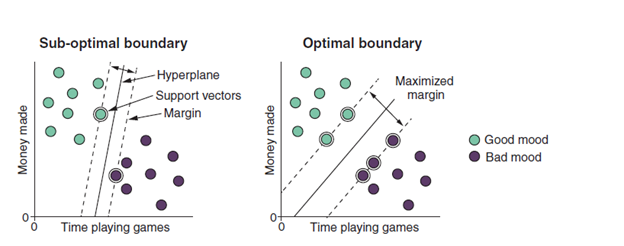
\includegraphics[width=8.67in]{svm1}

From the figure above, the SVM algorithm finds a hyperplane (solid line)
that passes through the feature space. An optimal hyperplane is one that
maximizes the margin around itself (dotted lines). The margin is a
region around the hyperplane that touches the fewest cases. Support
vectors are shown with double circles.

For a three-dimensional feature space, a hyperplane is a surface. It's
hard to picture hyperplanes in a four or more dimensional feature space,
but the principle is the same: they are surfaces that cut through the
feature space.

For problems where the classes are fully, linearly separable, there may
be many different hyperplanes that do just as good a job at separating
the classes in the training data. To find an optimal hyperplane (which
will, hopefully, generalize better to unseen data), the algorithm finds
the hyperplane that maximizes the margin around itself. The margin is a
distance around the hyperplane that touches the fewest training cases.
The cases in the data that touch the margin are called support vectors
because they support the position of the hyperplane (hence, the name of
the algorithm). The support vectors are the most important cases in the
training set because they define the boundary between the classes. Not
only this, but the hyperplane that the algorithm learns is entirely
dependent on the position of the support vectors and none of the other
cases in the training set. Take a look at figure 6.4. If we move the
position of one of the support vectors, then we move the position of the
hyperplane. If, however, we move a non-support vector case, there is no
influence on the hyperplane at all!

\begin{Shaded}
\begin{Highlighting}[]
\NormalTok{knitr}\SpecialCharTok{::}\FunctionTok{include\_graphics}\NormalTok{(}\StringTok{"svm2.png"}\NormalTok{)}
\end{Highlighting}
\end{Shaded}

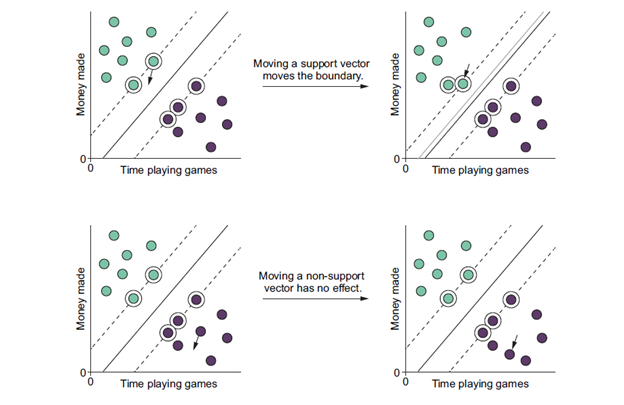
\includegraphics[width=8.67in]{svm2}

The position of the hyperplane is entirely dependent on the position of
support vectors. Moving a support vector moves the hyperplane from its
original position (dotted line) to a new position (top two plots).
Moving a non-support vector has no impact on the hyperplane (bottom two
plots).

SVMs are extremely popular right now. That's mainly for three reasons: *
They are good at finding ways of separating non-linearly separable
classes. * They tend to perform well for a wide variety of tasks. * We
now have the computational power to apply them to larger, more complex
datasets.

This last point is important because it highlights a potential downside
of SVMs: they tend to be more computationally expensive to train than
many other classification algorithms. For this reason, if you have a
very large dataset, and computational power is limited, it may be
economical for you to try cheaper algorithms first and see how they
perform.

\subsubsection{TIP}\label{tip-1}

Usually, we favor predictive performance over speed. But a
computationally cheap algorithm that performs well enough for your
problem may be preferable to you than one that is very expensive.
Therefore, I may try cheaper algorithms before trying the expensive
ones.

\subsubsection{How does the SVM algorithm find the optimal
hyperplane?}\label{how-does-the-svm-algorithm-find-the-optimal-hyperplane}

The math underpinning how SVMs work is complex, but if you're
interested, here are some of the basics of how the hyperplane is
learned. Recall from chapter 4 that the equation for a straight line can
be written as \(y = ax + b\), where a and b are the slope and
y-intercept of the line, respectively. We could rearrange this equation
to be \(y – ax – b = 0\) by shifting all the terms onto one side of the
equals sign. Using this formulation, we can say that any point that
falls on the line is one that satisfies this equation (the expression
will equal zero). You'll often see the equation for a hyperplane given
as \(wx + b = 0\), where w is the vector \((–b –a 1)\), x is the vector
(1 x y), and b is still the intercept. In the same way that any point
that lies on a straight line satisfies \(y – ax – b = 0\), any point
that falls on a hyperplane satisfies the equation \(wx + b = 0\). The
vector w is orthogonal or normal to the hyperplane. Therefore, by
changing the intercept, b, we can create new hyperplanes that are
parallel to the original. By changing b (and rescaling w) we can
arbitrarily define the hyperplanes that mark the margins as
\(wx + b = –1\) and \(wx + b = +1\). The distance between these margins
is given by 2/\textbar\textbar w\textbar\textbar, where
\textbar\textbar w\textbar\textbar{} is \(\sqrt {–b2 + –a2 + 12}\). As
we want to find the hyperplane that maximizes this distance, we need to
minimize \textbar\textbar w\textbar\textbar{} while ensuring that each
case is classified correctly. The algorithm does this by making sure all
cases in one class lie below \(wx + b = –1\) and all cases in the other
class lie above \(wx + b = +1\). A simple way of doing this is to
multiply the predicted value of each case by its corresponding label
(--1 or +1), making all outputs positive. This creates the constraint
that the margins must satisfy \(yi(wxi + b) \geq 1\). The SVM algorithm
therefore tries to solve the following minimization problem: minimize
\textbar\textbar w\textbar\textbar{} subject to \$ yi(wxi + b) \geq 1\$
for i = 1 \ldots{} N.

\subsection{What if the classes aren't fully
separable?}\label{what-if-the-classes-arent-fully-separable}

In the illustrations I've shown you so far, the classes have been fully
separable. This is so I could clearly show you how the positioning of
the hyperplane is chosen to maximize the margin. But what about
situations where the classes are not completely separable? How can the
algorithm find a hyperplane when there is no margin that won't have
cases inside it? The original formulation of SVMs uses what is often
referred to as a hard margin. If an SVM uses a hard margin, then no
cases are allowed to fall within the margin. This means that, if the
classes are not fully separable, the algorithm will fail. This is, of
course, a massive problem, because it relegates hard-margin SVM to
handling only ``easy'' classification problems where the training set
can be clearly partitioned into its component classes. As a result, an
extension to the SVM algorithm called soft-margin SVM is much more
commonly used. In soft-margin SVM, the algorithm still learns a
hyperplane that best separates the classes, but it allows cases to fall
inside its margin. The soft-margin SVM algorithm still tries to find the
hyperplane that best separates the classes, but it is penalized for
having cases inside its margin. How severe the penalty is for having a
case inside the margin is controlled by a hyperparameter that controls
how ``hard'' or ``soft'' the margin is (we'll discuss this
hyperparameter and how it affects the position of the hyperplane later
in the chapter). The harder the margin is, the fewer cases will be
inside it; the hyperplane will depend on a smaller number of support
vectors. The softer the margin is, the more cases will be inside it; the
hyperplane will depend on a larger number of support vectors. This has
consequences for the bias-variance trade-off: if our margin is too hard,
we might overfit the noise near the decision boundary, whereas if our
margin is too soft, we might underfit the data and learn a decision
boundary that does a bad job of separating the classes.

\subsubsection{SVMs for non-linearly separable
data}\label{svms-for-non-linearly-separable-data}

Great! So far the SVM algorithm seems quite simple---and for linearly
separable classes like in our boss-mood example, it is. But I mentioned
that one of the strengths of the SVM algorithm is that it can learn
decision boundaries between classes that are not linearly separable.
I've told you that the algorithm learns linear hyperplanes, so this
seems like a contradiction. Well, here's what makes the SVM algorithm so
powerful: it can add an extra dimension to your data to find a linear
way to separate nonlinear data. Take a look at the example in figure
6.5. The classes are not linearly separable using the two predictor
variables. The SVM algorithm adds an extra dimension to the data, such
that a linear hyperplane can separate the classes in this new,
higher-dimensional space. We can visualize this as a sort of deformation
or stretching of the feature space. The extra dimension is called a
kernel.

\subsubsection{NOTE}\label{note-12}

Recall from chapter 5 that discriminant analysis condenses the
information from the predictor variables into a smaller number of
variables. Contrast this to the SVM algorithm, which expands the
information from the predictor variables into an extra variable!

\subsubsection{Why is it called a
kernel?}\label{why-is-it-called-a-kernel}

The word kernel may confuse you (it certainly confuses me). It has
nothing to do with the kernel in computing (the bit of your operating
system that directly interfaces with the computer hardware), or kernels
in corn or fruit. The truth is that the reason they are called kernels
is murky. In 1904, a German mathematician named David Hilbert published
Grundzüge einer allgemeinen theorie der linearen integralgleichungen
(Principles of a general theory of linear integral equations). In this
book, Hilbert uses the word kern to mean the core of an integral
equation. In 1909, an American mathematician called Maxime Bôcher
published An introduction to the study of integral equations in which he
translates Hilbert's use of the word kern to kernel. The mathematics of
kernel functions evolved from the work in these publications and took
the name kernel with them. The extremely confusing thing is that
multiple, seemingly unrelated concepts in mathematics include the word
kernel!

How does the algorithm find this new kernel? It uses a mathematical
transformation of the data called a kernel function. There are many
kernel functions to choose from, each of which applies a different
transformation to the data and is suitable for finding linear decision
boundaries for different situations. Figure 6.6 shows examples of
situations where some common kernel functions can separate non-linearly
separable data:

\begin{itemize}
\tightlist
\item
  Linear kernel (equivalent to no kernel)
\item
  Polynomial kernel
\item
  Gaussian radial basis kernel
\item
  Sigmoid kernel
\end{itemize}

The type of kernel function for a given problem isn't learned from the
data---we have to specify it. Because of this, the choice of kernel
function is a categorical hyperparameter (a hyperparameter that takes
discrete, not continuous values). Therefore, the best approach for
choosing the best-performing kernel is with hyperparameter tuning.

\begin{Shaded}
\begin{Highlighting}[]
\NormalTok{knitr}\SpecialCharTok{::}\FunctionTok{include\_graphics}\NormalTok{(}\StringTok{"svm3.png"}\NormalTok{)}
\end{Highlighting}
\end{Shaded}

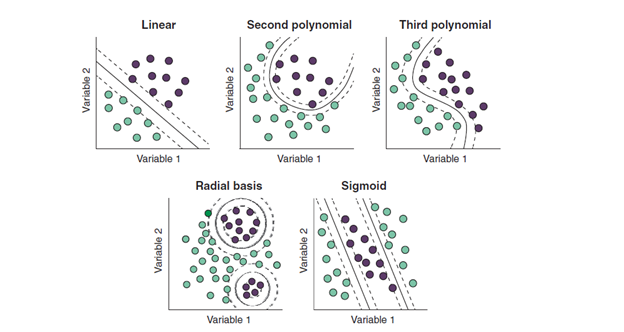
\includegraphics[width=8.67in]{svm3}

\subsection{Hyperparameters of the SVM
algorithm}\label{hyperparameters-of-the-svm-algorithm}

This is where SVMs become fun/difficult/painful, depending on your
problem, computational budget, and sense of humor. We need to tune quite
a lot of hyperparameters when building an SVM. This, coupled with the
fact that training a single model can be moderately expensive, can make
training an optimally performing SVM take quite a long time. You'll see
this in the worked example in section 6.5.2. So the SVM algorithm has
quite a few hyperparameters to tune, but the most important ones to
consider are as follows:

\begin{itemize}
\tightlist
\item
  The kernel hyperparameter (shown in figure 6.6)
\item
  The degree hyperparameter, which controls how ``bendy'' the decision
  boundary will be for the polynomial kernel (shown in figure 6.6)
\item
  The cost or C hyperparameter, which controls how ``hard'' or ``soft''
  the margin is (shown in figure 6.7)
\item
  The gamma hyperparameter, which controls how much influence individual
  cases have on the position of the decision boundary (shown in figure
  6.7)
\end{itemize}

The effects of the kernel function and degree hyperparameter are shown
in figure 6.6. Note the difference in the shape of the decision boundary
between the second- and third-degree polynomials.

\subsubsection{NOTE}\label{note-13}

The higher the degree of the polynomial, the more bendy and complex a
decision boundary can be learned, but this has the potential to overfit
the training set.

The cost (also called C) hyperparameter in soft-margin SVMs assigns a
cost or penalty to having cases inside the margin or, put another way,
tells the algorithm how bad it is to have cases inside the margin. A low
cost tells the algorithm that it's acceptable to have more cases inside
the margin and will result in wider margins that are less influenced by
local differences near the class boundary. A high cost imposes a harsher
penalty on having cases inside the boundary and will result in narrower
margins that are more influenced by local differences near the class
boundary. The effect of cost is illustrated for a linear kernel in the
top part of figure 6.6.

\subsubsection{NOTE}\label{note-14}

Cases inside the margin are also support vectors, as moving them would
change the position of the hyperplane.

The gamma hyperparameter controls the influence that each case has on
the position of the hyperplane and is used by all the kernel functions
except the linear kernel. Think of each case in the training set jumping
up and down shouting, ``Me! Me! Classify me correctly!'' The larger
gamma is, the more attention-seeking each case is, and the more granular
the decision boundary will be (potentially leading to overfitting). The
smaller gamma is, the less attention-seeking each case will be, and the
less granular the decision boundary will be (potentially leading to
underfitting). The effect of gamma is illustrated for a Gaussian radial
basis kernel in the bottom part of figure 6.7.

\begin{Shaded}
\begin{Highlighting}[]
\NormalTok{knitr}\SpecialCharTok{::}\FunctionTok{include\_graphics}\NormalTok{(}\StringTok{"svm4.png"}\NormalTok{)}
\end{Highlighting}
\end{Shaded}

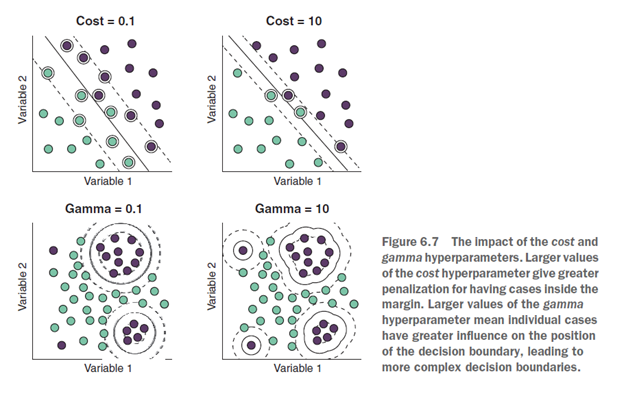
\includegraphics[width=8.67in]{svm4}

So the SVM algorithm has multiple hyperparameters to tune! I'll show you
how we can tune these simultaneously using mlr in section 6.5.2.

\subsubsection{What if we have more than two
classes?}\label{what-if-we-have-more-than-two-classes-1}

So far, I've only shown you examples of two-class classification
problems. This is because the SVM algorithm is inherently geared toward
separating two classes. But can we use it for multiclass problems (where
we're trying to predict more than two classes)? Absolutely! When there
are more than two classes, instead of creating a single SVM, we make
multiple models and let them fight it out to predict the most likely
class for new data. There are two ways of doing this:

\begin{itemize}
\tightlist
\item
  One-versus-all
\item
  One-versus-one
\end{itemize}

In the one-versus-all (also called one versus rest) approach, we create
as many SVM models as there are classes. Each SVM model describes a
hyperplane that best separates one class from all the other classes.
Hence the name, one-versus-all. When we classify new, unseen cases, the
models play a game of winner takes all. Put simply, the model that puts
the new case on the ``correct'' side of its hyperplane (the side with
the class it separates from all the others) wins. The case is then
assigned to the class that the model was trying to separate from the
others. This is illustrated in the plot on the left in figure 6.8.

\begin{Shaded}
\begin{Highlighting}[]
\NormalTok{knitr}\SpecialCharTok{::}\FunctionTok{include\_graphics}\NormalTok{(}\StringTok{"svm5.png"}\NormalTok{)}
\end{Highlighting}
\end{Shaded}

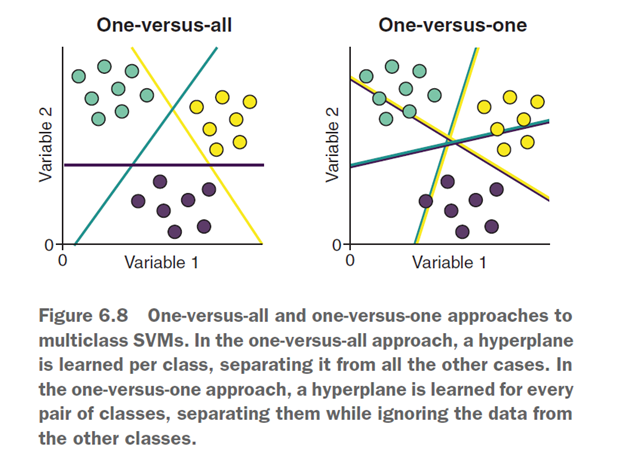
\includegraphics[width=8.67in]{svm5}

In the one-versus-one approach, we create an SVM model for every pair of
classes. Each SVM model describes a hyperplane that best separates one
class from one other class, ignoring data from the other classes. Hence,
the name, one-versus-one. When we classify new, unseen cases, each model
casts a vote. For example, if one model separatesclasses A and B, and
the new data falls on the B side of the decision boundary, that model
will vote for B. This continues for all the models, and the majority
class vote wins. This is illustrated in the plot on the right in figure
6.8. Which do we choose? Well in practice, there is usually little
difference in the performance of the two methods. Despite training more
models (for more than three classes), one-versus-one is sometimes less
computationally expensive than one-versusall.

This is because, although we're training more models, the training sets
are smaller (because of the ignored cases). The implementation of the
SVM algorithm called by mlr uses the one-versus-one approach. There is,
however, a problem with these approaches. There will often be regions of
the feature space in which none of the models gives a clear winning
class. Can you see the triangular space between the hyperplanes on the
left in figure 6.8? If a new case appeared inside this triangle, none of
the three models would clearly win outright. This is a sort of
classification no-man's land. Though not as obvious in figure 6.8, this
also occurs with the one-versus-one approach.

If there is no outright winner when predicting a new case, a technique
called Platt scaling is used (named after computer scientist John
Platt). Platt scaling takes the distances of the cases from each
hyperplane and converts them into probabilities using the logistic
function. Recall from chapter 4 that the logistic function maps a
continuous variable to probabilities between 0 and 1. Using Platt
scaling to make predictions proceeds like this:

1 For every hyperplane (whether we use one-versus-all or
one-versus-one): a) Measure the distance of each case from the
hyperplane. b) Use the logistic function to convert these distances into
probabilities.

2 Classify new data as belonging to the class of the hyperplane that has
the highest probability.

If this seems confusing, take a look at figure 6.9. We're using the
one-versus-all approach in the figure, and we have generated three
separate hyperplanes (one to separate each class from the rest). The
dashed arrows in the figure indicate distance in either direction, away
from the hyperplanes. Platt scaling converts these distances into
probabilities using the logistic function (the class each hyperplane
separates from the rest has positive distance).

When we classify new, unseen data, the distance of the new data is
converted into a probability using each of the three S-shaped curves,
and the case is classified as the one that gives the highest
probability. Handily, all of this is taken care of for us in the
implementation of SVM called by mlr. If we supply a three-class
classification task, we will get a one-versus-one SVM model with Platt
scaling without having to change our code.

\begin{Shaded}
\begin{Highlighting}[]
\NormalTok{knitr}\SpecialCharTok{::}\FunctionTok{include\_graphics}\NormalTok{(}\StringTok{"svm6.png"}\NormalTok{)}
\end{Highlighting}
\end{Shaded}

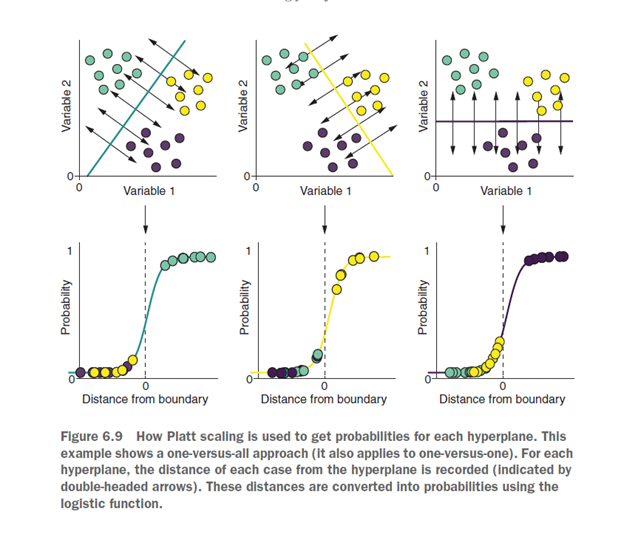
\includegraphics[width=8.67in]{svm6}

\subsection{Building your first SVM
model}\label{building-your-first-svm-model}

In this section, I'll teach you how to build an SVM model and tune
multiple hyperparameters simultaneously. Imagine that you're sick and
tired of receiving so many spam emails (maybe you don't need to
imagine!). It's difficult for you to be productive because you get so
many emails requesting your bank details for a mysterious Ugandan
inheritance, and trying to sell you Viagra. You decide to perform a
feature extraction on the emails you receive over a few months, which
you manually class as spam or not spam. These features include things
like the number of exclamation marks and the frequency of certain words.
With this data, you want to make an SVM that you can use as a spam
filter, which will classify new emails as spam or not spam. In this
section, you'll learn how to train an SVM model and tune multiple
hyperparameters simultaneously. Let's start by loading the mlr and
tidyverse packages:

\begin{Shaded}
\begin{Highlighting}[]
\FunctionTok{library}\NormalTok{(mlr)}
\FunctionTok{library}\NormalTok{(tidyverse)}
\end{Highlighting}
\end{Shaded}

Now let's load the data, which is built into the kernlab package,
convert it into a tibble (with as\_tibble()), and explore it.

\subsubsection{NOTE}\label{note-15}

The kernlab package should have been installed along with mlr as a
suggested package. If you get an error when trying to load the data, you
may need to install it with install.packages(``kernlab'').

We have a tibble containing 4,601 emails and 58 variables extracted from
emails. Our goal is to train a model that can use the information in
these variables to predict whether a new email is spam or not.

\subsubsection{NOTE}\label{note-16}

Except for the factor type, which denotes whether an email is spam, all
of the variables are continuous, because the SVM algorithm cannot handle
categorical predictors.

\begin{Shaded}
\begin{Highlighting}[]
\FunctionTok{data}\NormalTok{(spam, }\AttributeTok{package =} \StringTok{"kernlab"}\NormalTok{)}
\NormalTok{spamTib }\OtherTok{\textless{}{-}} \FunctionTok{as\_tibble}\NormalTok{(spam)}
\NormalTok{spamTib}
\end{Highlighting}
\end{Shaded}

\begin{verbatim}
# A tibble: 4,601 x 58
    make address   all num3d   our  over remove internet order  mail receive
   <dbl>   <dbl> <dbl> <dbl> <dbl> <dbl>  <dbl>    <dbl> <dbl> <dbl>   <dbl>
 1  0       0.64  0.64     0  0.32  0      0        0     0     0       0   
 2  0.21    0.28  0.5      0  0.14  0.28   0.21     0.07  0     0.94    0.21
 3  0.06    0     0.71     0  1.23  0.19   0.19     0.12  0.64  0.25    0.38
 4  0       0     0        0  0.63  0      0.31     0.63  0.31  0.63    0.31
 5  0       0     0        0  0.63  0      0.31     0.63  0.31  0.63    0.31
 6  0       0     0        0  1.85  0      0        1.85  0     0       0   
 7  0       0     0        0  1.92  0      0        0     0     0.64    0.96
 8  0       0     0        0  1.88  0      0        1.88  0     0       0   
 9  0.15    0     0.46     0  0.61  0      0.3      0     0.92  0.76    0.76
10  0.06    0.12  0.77     0  0.19  0.32   0.38     0     0.06  0       0   
# i 4,591 more rows
# i 47 more variables: will <dbl>, people <dbl>, report <dbl>, addresses <dbl>,
#   free <dbl>, business <dbl>, email <dbl>, you <dbl>, credit <dbl>,
#   your <dbl>, font <dbl>, num000 <dbl>, money <dbl>, hp <dbl>, hpl <dbl>,
#   george <dbl>, num650 <dbl>, lab <dbl>, labs <dbl>, telnet <dbl>,
#   num857 <dbl>, data <dbl>, num415 <dbl>, num85 <dbl>, technology <dbl>,
#   num1999 <dbl>, parts <dbl>, pm <dbl>, direct <dbl>, cs <dbl>, ...
\end{verbatim}

\subsubsection{TIP}\label{tip-2}

This dataset has a lot of features! I'm not going to discuss the meaning
of each one, but you can see a description of what they mean by running

\begin{Shaded}
\begin{Highlighting}[]
\DocumentationTok{\#\#?kernlab::spam.}
\end{Highlighting}
\end{Shaded}

\subsubsection{Tuning our
hyperparameters}\label{tuning-our-hyperparameters}

Let's define our task and learner. This time, we supply ``classif.svm''
as the argument to makeLearner() to specify that we're going to use SVM.

\paragraph{Create the task and
learner}\label{create-the-task-and-learner}

\begin{Shaded}
\begin{Highlighting}[]
\NormalTok{spamTask }\OtherTok{\textless{}{-}} \FunctionTok{makeClassifTask}\NormalTok{(}\AttributeTok{data =}\NormalTok{ spamTib, }\AttributeTok{target =} \StringTok{"type"}\NormalTok{)}
\NormalTok{svm }\OtherTok{\textless{}{-}} \FunctionTok{makeLearner}\NormalTok{(}\StringTok{"classif.svm"}\NormalTok{)}
\end{Highlighting}
\end{Shaded}

Before we train our model, we need to tune our hyperparameters. To find
out which hyperparameters are available for tuning for an algorithm, we
simply pass the name of the algorithm in quotes to getParamSet(). For
example, listing 6.9 shows how to print the hyperparameters for the SVM
algorithm. I've removed some rows and columns of the output to make it
fit, but the most important columns are there: * The row name is the
name of the hyperparameter. * Type is whether the hyperparameter takes
numeric, integer, discrete, or logical values. * Def is the default
value (the value that will be used if you don't tune the
hyperparameter). * Constr defines the constraints for the
hyperparameter: either a set of specific values or a range of acceptable
values. * Req defines whether the hyperparameter is required by the
learner. * Tunable is logical and defines whether that hyperparameter
can be tuned (some algorithms have options that cannot be tuned but can
be set by the user).

\subsubsection{Printing available SVM
hyperparameters}\label{printing-available-svm-hyperparameters}

\begin{Shaded}
\begin{Highlighting}[]
\FunctionTok{getParamSet}\NormalTok{(}\StringTok{"classif.svm"}\NormalTok{)}
\end{Highlighting}
\end{Shaded}

\begin{verbatim}
                       Type  len             Def
type               discrete    - C-classifica...
cost                numeric    -               1
nu                  numeric    -             0.5
class.weights numericvector <NA>               -
kernel             discrete    -          radial
degree              integer    -               3
coef0               numeric    -               0
gamma               numeric    -               -
cachesize           numeric    -              40
tolerance           numeric    -           0.001
shrinking           logical    -            TRUE
cross               integer    -               0
fitted              logical    -            TRUE
scale         logicalvector <NA>            TRUE
                                          Constr Req Tunable Trafo
type          C-classification,nu-classification   -    TRUE     -
cost                                    0 to Inf   Y    TRUE     -
nu                                   -Inf to Inf   Y    TRUE     -
class.weights                           0 to Inf   -    TRUE     -
kernel          linear,polynomial,radial,sigmoid   -    TRUE     -
degree                                  1 to Inf   Y    TRUE     -
coef0                                -Inf to Inf   Y    TRUE     -
gamma                                   0 to Inf   Y    TRUE     -
cachesize                            -Inf to Inf   -    TRUE     -
tolerance                               0 to Inf   -    TRUE     -
shrinking                                      -   -    TRUE     -
cross                                   0 to Inf   -   FALSE     -
fitted                                         -   -   FALSE     -
scale                                          -   -    TRUE     -
\end{verbatim}

The SVM algorithm is sensitive to variables being on different scales,
so it's usually a good idea to scale the predictors first. Notice the
scale hyperparameter: it tells us that the algorithm will scale the data
for us by default.

\subsubsection{Extracting the possible values for a
hyperparameter}\label{extracting-the-possible-values-for-a-hyperparameter}

While the getParamSet() function is useful, I don't find it particularly
simple to extract information from. If you call
str(getParamSet(``classif.svm'')), you'll see that it has a reasonably
complex structure. To extract information about a particular
hyperparameter, you need to call
getParam-Set(``classif.svm'')\(pars\){[}HYPERPAR{]} (where
{[}HYPERPAR{]} is replaced by the hyperparameter you're interested in).
To extract the possible values for that hyperparameter, you append
\$values to the call. For example, the following extracts the possible
kernel functions:

\begin{Shaded}
\begin{Highlighting}[]
\FunctionTok{getParamSet}\NormalTok{(}\StringTok{"classif.svm"}\NormalTok{)}\SpecialCharTok{$}\NormalTok{pars}\SpecialCharTok{$}\NormalTok{kernel}\SpecialCharTok{$}\NormalTok{values}
\end{Highlighting}
\end{Shaded}

\begin{verbatim}
$linear
[1] "linear"

$polynomial
[1] "polynomial"

$radial
[1] "radial"

$sigmoid
[1] "sigmoid"
\end{verbatim}

These are the most important hyperparameters for us to tune: * Kernel *
Cost * Degree * Gamma

Listing 6.10 defines the hyperparameters we want to tune. We're going to
start by defining a vector of kernel functions we wish to tune.

TIP Notice that I omit the linear kernel. This is because the linear
kernel is the same as the polynomial kernel with degree = 1, so we'll
just make sure we include 1 as a possible value for the degree
hyperparameter. Including the linear kernel and the first-degree
polynomial kernel is simply a waste of computing time. Next, we use the
makeParamSet() function to define the hyperparameter space we wish to
tune over. To the makeParamSet() function, we supply the information
needed to define each hyperparameter we wish to tune, separated by
commas. Let's break this down line by line:

\begin{itemize}
\item
  The kernel hyperparameter takes discrete values (the name of the
  kernel function), so we use the makeDiscreteParam() function to define
  its values as the vector of kernels we created.
\item
  The degree hyperparameter takes integer values (whole numbers), so we
  use the makeIntegerParam() function and define the lower and upper
  values we wish to tune over.
\item
  The cost and gamma hyperparameters take numeric values (any number
  between zero and infinity), so we use the makeNumericParam() function
  to define the lower and upper values we wish to tune over.
\end{itemize}

For each of these functions, the first argument is the name of the
hyperparameter given by getParamSet(``classif.svm''), in quotes.

\subsubsection{Defining the hyperparameter space for
tuning}\label{defining-the-hyperparameter-space-for-tuning}

\begin{Shaded}
\begin{Highlighting}[]
\NormalTok{kernels }\OtherTok{\textless{}{-}} \FunctionTok{c}\NormalTok{(}\StringTok{"polynomial"}\NormalTok{, }\StringTok{"radial"}\NormalTok{, }\StringTok{"sigmoid"}\NormalTok{)}
\NormalTok{svmParamSpace }\OtherTok{\textless{}{-}} \FunctionTok{makeParamSet}\NormalTok{(}
  \FunctionTok{makeDiscreteParam}\NormalTok{(}\StringTok{"kernel"}\NormalTok{, }\AttributeTok{values =}\NormalTok{ kernels),}
  \FunctionTok{makeIntegerParam}\NormalTok{(}\StringTok{"degree"}\NormalTok{, }\AttributeTok{lower =} \DecValTok{1}\NormalTok{, }\AttributeTok{upper =} \DecValTok{3}\NormalTok{),}
  \FunctionTok{makeNumericParam}\NormalTok{(}\StringTok{"cost"}\NormalTok{, }\AttributeTok{lower =} \FloatTok{0.1}\NormalTok{, }\AttributeTok{upper =} \DecValTok{10}\NormalTok{),}
  \FunctionTok{makeNumericParam}\NormalTok{(}\StringTok{"gamma"}\NormalTok{, }\AttributeTok{lower =} \FloatTok{0.1}\NormalTok{, }\DecValTok{10}\NormalTok{))}
\end{Highlighting}
\end{Shaded}

\begin{Shaded}
\begin{Highlighting}[]
\NormalTok{svmParamSpace}
\end{Highlighting}
\end{Shaded}

\begin{verbatim}
           Type len Def                    Constr Req Tunable Trafo
kernel discrete   -   - polynomial,radial,sigmoid   -    TRUE     -
degree  integer   -   -                    1 to 3   -    TRUE     -
cost    numeric   -   -                 0.1 to 10   -    TRUE     -
gamma   numeric   -   -                 0.1 to 10   -    TRUE     -
\end{verbatim}

Cast your mind back to chapter 3, when we tuned k for the kNN algorithm.
We used the grid search procedure during tuning to try every value of k
that we defined. This is what the grid search method does: it tries
every combination of the hyperparameter space you define and finds the
best-performing combination. Grid search is great because, provided you
specify a sensible hyperparameter space to search over, it will always
find the best-performing hyperparameters. But look at the hyperparameter
space we defined for our SVM. Let's say we wanted to try values for the
cost and gamma hyperparameters from 0.1 to 10, in steps of 0.1 (that's
100 values of each). We're trying three kernel functions and three
values of the degree hyperparameter. To perform a grid search over this
parameter space would require training a model 90,000 times! In such a
situation, if you have the time, patience, and computational budget for
such a grid search, then good for you. I, for one, have better things I
could be doing with my computer! Instead, we can employ a technique
called random search. Rather than trying every possible combination of
parameters, random search proceeds as follows:

1 Randomly select a combination of hyperparameter values. 2 Use
cross-validation to train and evaluate a model using those
hyperparameter values. 3 Record the performance metric of the model
(usually mean misclassification error for classification tasks). 4
Repeat (iterate) steps 1 to 3 as many times as your computational budget
allows. 5 Select the combination of hyperparameter values that gave you
the bestperforming model.

Unlike grid search, random search isn't guaranteed to find the best set
of hyperparameter values. However, with enough iterations, it can
usually find a good combination that performs well. By using random
search, we can run 500 combinations of hyperparameter values, instead of
all 90,000 combinations. Let's define our random search using the
makeTuneControlRandom() function. We use the maxit argument to tell the
function how many iterations of the random search procedure we want to
use. You should try to set this as high as your computational budget
allows, but in this example we'll stick to 20 to prevent the example
from taking too long. Next, we describe our cross-validation procedure.
Remember I said in chapter 3 that I prefer k-fold cross-validation
unless the process is computationally expensive. Well, this is
computationally expensive, so we're compromising by using holdout
cross-validation instead.

\subsection{Defining the random
search}\label{defining-the-random-search}

\begin{Shaded}
\begin{Highlighting}[]
\NormalTok{randSearch }\OtherTok{\textless{}{-}} \FunctionTok{makeTuneControlRandom}\NormalTok{(}\AttributeTok{maxit =} \DecValTok{20}\NormalTok{)}
\NormalTok{cvForTuning }\OtherTok{\textless{}{-}} \FunctionTok{makeResampleDesc}\NormalTok{(}\StringTok{"Holdout"}\NormalTok{, }\AttributeTok{split =} \DecValTok{2}\SpecialCharTok{/}\DecValTok{3}\NormalTok{)}
\end{Highlighting}
\end{Shaded}

There's something else we can do to speed up this process. R, as a
language, doesn't make that much use of multithreading (using multiple
CPUs simultaneously to accomplish a task). However, one of the benefits
of the mlr package is that it allows multithreading to be used with its
functions. This helps you use multiple cores/CPUs on your computer to
accomplish tasks such as hyperparameter tuning and cross-validation much
more quickly.

TIP If you don't know how many cores your computer has, you can find out
in R by running parallel::detectCores(). (If your computer only has one
core, the 90s called---they want their computer back.)

To run an mlr process in parallel, we place its code between the
parallelStart-Socket() and parallelStop() functions from the parallelMap
package. To start our hyperparameter tuning process, we call the
tuneParams() function and supply the following as arguments:

\begin{itemize}
\tightlist
\item
  First argument = name of the learner
\item
  task = name of our task
\item
  resampling = cross-validation procedure (defined in listing 6.11)
\item
  par.set = hyperparameter space (defined in listing 6.10)
\item
  control = search procedure (random search, defined in listing 6.11)
\end{itemize}

This code between the parallelStartSocket() and parallelStop() functions
is shown in listing 6.12. Notice that the downside of running
cross-validation processes in parallel is that we no longer get a
running update of how far we've got.

WARNING The computer I'm writing this on has four cores, and this code
takes nearly a minute to run on it. It is of the utmost importance that
you go make a cup of tea while it runs. Milk and no sugar, please.

\subsection{Performing hyperparameter
tuning}\label{performing-hyperparameter-tuning}

\begin{Shaded}
\begin{Highlighting}[]
\FunctionTok{library}\NormalTok{(parallelMap)}
\FunctionTok{library}\NormalTok{(parallel)}
\FunctionTok{parallelStartSocket}\NormalTok{(}\AttributeTok{cpus =} \FunctionTok{detectCores}\NormalTok{())}
\NormalTok{tunedSvmPars }\OtherTok{\textless{}{-}} \FunctionTok{tuneParams}\NormalTok{(}\StringTok{"classif.svm"}\NormalTok{, }\AttributeTok{task =}\NormalTok{ spamTask,}
                           \AttributeTok{resampling =}\NormalTok{ cvForTuning,}
                           \AttributeTok{par.set =}\NormalTok{ svmParamSpace,}
                           \AttributeTok{control =}\NormalTok{ randSearch)}
\FunctionTok{parallelStop}\NormalTok{()}
\end{Highlighting}
\end{Shaded}

TIP The degree hyperparameter only applies to the polynomial kernel
function, and the gamma hyperparameter doesn't apply to the linear
kernel. Does this create errors when the random search selects
combinations that don't make sense? Nope. If the random search selects
the sigmoid kernel, for example, it simply ignores the value of the
degree hyperparameter.

Welcome back after our interlude! You can print the best-performing
hyperparameter values and the performance of the model built with them
by calling tunedSvm, or extract just the named values (so you can train
a new model using them) by calling tunedSvm\$x. Looking at the following
listing, we can see that the first-degree polynomial kernel function
(equivalent to the linear kernel function) gave the model that performs
the best, with a cost of 8.6 and gamma of 5.75.

\subsubsection{Extracting the winning hyperparameter values from
tuning}\label{extracting-the-winning-hyperparameter-values-from-tuning}

\begin{Shaded}
\begin{Highlighting}[]
\NormalTok{tunedSvmPars}
\end{Highlighting}
\end{Shaded}

\begin{verbatim}
Tune result:
Op. pars: kernel=polynomial; degree=1; cost=7.71; gamma=4.1
mmce.test.mean=0.0638853
\end{verbatim}

Your values are probably different than mine. This is the nature of the
random search: it may find different winning combinations of
hyperparameter values each time it's run. To reduce this variance, we
should commit to increasing the number of iterations the search makes.

\subsubsection{Training the model with the tuned
hyperparameters}\label{training-the-model-with-the-tuned-hyperparameters}

Now that we've tuned our hyperparameters, let's build our model using
the bestperforming combination. Recall from chapter 3 that we use the
setHyperPars() function to combine a learner with a set of predefined
hyperparameter values. The first argument is the learner we want to use,
and the par.vals argument is the object containing our tuned
hyperparameter values. We then train a model using our tuned- Svm
learner with the train() function.

\begin{Shaded}
\begin{Highlighting}[]
\NormalTok{tunedSvm }\OtherTok{\textless{}{-}} \FunctionTok{setHyperPars}\NormalTok{(}\FunctionTok{makeLearner}\NormalTok{(}\StringTok{"classif.svm"}\NormalTok{),}
                         \AttributeTok{par.vals =}\NormalTok{ tunedSvmPars}\SpecialCharTok{$}\NormalTok{x)}
\NormalTok{tunedSvmModel }\OtherTok{\textless{}{-}} \FunctionTok{train}\NormalTok{(tunedSvm, spamTask)}
\end{Highlighting}
\end{Shaded}

\subsection{View the model with the tuned
parameters}\label{view-the-model-with-the-tuned-parameters}

\begin{Shaded}
\begin{Highlighting}[]
\NormalTok{tunedSvmModel}
\end{Highlighting}
\end{Shaded}

\begin{verbatim}
Model for learner.id=classif.svm; learner.class=classif.svm
Trained on: task.id = spamTib; obs = 4601; features = 57
Hyperparameters: kernel=polynomial,degree=1,cost=7.71,gamma=4.1
\end{verbatim}

TIP Because we already defined our learner in listing 6.8, we could
simply have run setHyperPars(svm, par.vals = tunedSvmPars\$x) to achieve
the same result.

\subsubsection{Cross-validating our SVM
model}\label{cross-validating-our-svm-model}

We've built a model using tuned hyperparameters. In this section, we'll
cross-validate the model to estimate how it will perform on new, unseen
data. Recall from chapter 3 that it's important to cross-validate the
entire model-building process. This means any data-dependent steps in
our model-building process (such as hyperparameter tuning) need to be
included in our cross-validation. If we don't include them, our
cross-validation is likely to give an overoptimistic estimate (a biased
estimate) of how well the model will perform.

TIP What counts as a data-independent step in model building? Things
like removing nonsense variables by hand, changing variable names and
types, and replacing a missing value code with NA. These steps are
data-independent because they would be the same regardless of the values
in the data.

Recall also that to include hyperparameter tuning in our
cross-validation, we need to use a wrapper function that wraps together
our learner and hyperparameter tuning process. The cross-validation
process is shown in listing 6.15. Because mlr will use nested
cross-validation (where hyperparameter tuning is performed in the inner
loop, and the winning combination of values is passed to the outer
loop), we first define our outer cross-validation strategy using the
makeResamplDesc() function. In this example, I've chosen 3-fold
cross-validation for the outer loop. For the inner loop, we'll use the
cvForTuning resampling description defined in listing 6.11 (holdout
cross-validation with a 2/3 split).

Next, we make our wrapped learner using the makeTuneWrapper() function.
The arguments are as follows: * First argument = name of the learner *
resampling = inner loop cross-validation strategy * par.set =
hyperparameter space (defined in listing 6.10) * control = search
procedure (defined in listing 6.11)

As the cross-validation will take a while, it's prudent to start
parallelization with the parallelStartSocket() function. Now, to run our
nested cross-validation, we call the resample() function, where the
first argument is our wrapped learner, the second argument is our task,
and the third argument is our outer cross-validation strategy.

WARNING This takes a little over a minute on my four-core computer. In
the meantime, you know what to do. Milk and no sugar, please. Do you
have any cake?

\subsubsection{Cross-validating the model-building
process}\label{cross-validating-the-model-building-process}

\begin{Shaded}
\begin{Highlighting}[]
\NormalTok{outer }\OtherTok{\textless{}{-}} \FunctionTok{makeResampleDesc}\NormalTok{(}\StringTok{"CV"}\NormalTok{, }\AttributeTok{iters =} \DecValTok{3}\NormalTok{)}
\NormalTok{svmWrapper }\OtherTok{\textless{}{-}} \FunctionTok{makeTuneWrapper}\NormalTok{(}\StringTok{"classif.svm"}\NormalTok{, }\AttributeTok{resampling =}\NormalTok{ cvForTuning,}
                              \AttributeTok{par.set =}\NormalTok{ svmParamSpace,}
                              \AttributeTok{control =}\NormalTok{ randSearch)}
\end{Highlighting}
\end{Shaded}

\begin{Shaded}
\begin{Highlighting}[]
\FunctionTok{parallelStartSocket}\NormalTok{(}\AttributeTok{cpus =} \FunctionTok{detectCores}\NormalTok{())}
\NormalTok{cvWithTuning }\OtherTok{\textless{}{-}} \FunctionTok{resample}\NormalTok{(svmWrapper, spamTask, }\AttributeTok{resampling =}\NormalTok{ outer, }
                         \AttributeTok{measures =} \FunctionTok{list}\NormalTok{(mmce, acc, fpr, fnr))}
\FunctionTok{parallelStop}\NormalTok{()}
\end{Highlighting}
\end{Shaded}

Now let's take a look at the result of our cross-validation procedure by
printing the contents of the cvWithTuning object. \#\#\# Extracting the
cross-validation result

\begin{Shaded}
\begin{Highlighting}[]
\NormalTok{cvWithTuning}
\end{Highlighting}
\end{Shaded}

\begin{verbatim}
Resample Result
Task: spamTib
Learner: classif.svm.tuned
Aggr perf: mmce.test.mean=0.0715036,acc.test.mean=0.9284964,fpr.test.mean=0.1024528,fnr.test.mean=0.0513175
Runtime: 59.5436
\end{verbatim}

We're correctly classifying 1 -- 0.0738965 = 0.9261 = 92.61\% of emails
as spam or not spam. Not bad for a first attempt!

The performance metrics indicate a well-performing Support Vector
Machine model on the test data. Here's a breakdown of each metric and
its interpretation in this context:

\subsubsection{mmce.test.mean (Mean Misclassification
Error):}\label{mmce.test.mean-mean-misclassification-error}

0.0711 represents the average proportion of mistakes your model made on
the test data. In other words, the model misclassified roughly 7.1\% of
the observations.

\subsubsection{acc.test.mean
(Accuracy):}\label{acc.test.mean-accuracy-1}

0.9289 signifies the overall correctness of your model. The model
correctly classified approximately 92.9\% of the observations in the
test set. This is a good accuracy metric.

\subsubsection{fpr.test.mean (False Positive
Rate):}\label{fpr.test.mean-false-positive-rate-1}

0.1063 represents the average proportion of negative cases (actual
negatives) that the model incorrectly classified as positive. This
reflects the rate of ``false alarms.'' A higher fpr indicates the model
is more likely to identify negative cases as positive. Here, it's around
10.6\%.

\subsubsection{fnr.test.mean (False Negative
Rate):}\label{fnr.test.mean-false-negative-rate-1}

0.0480 represents the average proportion of positive cases (actual
positives) that the model incorrectly classified as negative. It
reflects the rate of ``missed cases.'' A lower fnr is preferable, and
here it's around 4.8\%.

\subsection{Overall, these metrics
suggest:}\label{overall-these-metrics-suggest-1}

The SVM model performs well, with a low misclassification error and high
accuracy on the test data. The model is slightly more likely to
misclassify negative cases as positive (higher fpr than fnr). This might
be acceptable depending on the specific application. For instance, if
the cost of missing a positive case is much higher, a lower fnr is
crucial.

Here are some additional points to consider:

It's essential to understand the context of your problem. These metrics
provide a general idea of how well the model performs on unseen data.
Depending on the application, some metrics might hold more weight. For
example, in medical diagnosis, minimizing false negatives (missing
actual positive cases) is critical.

\subsubsection{View the
Misclassification}\label{view-the-misclassification}

\begin{Shaded}
\begin{Highlighting}[]
\NormalTok{cvWithTuning}\SpecialCharTok{$}\NormalTok{aggr}
\end{Highlighting}
\end{Shaded}

\begin{verbatim}
mmce.test.mean  acc.test.mean  fpr.test.mean  fnr.test.mean 
    0.07150356     0.92849644     0.10245278     0.05131751 
\end{verbatim}

\subsubsection{View the Classification
Accuracy}\label{view-the-classification-accuracy}

\begin{Shaded}
\begin{Highlighting}[]
\DecValTok{1} \SpecialCharTok{{-}}\NormalTok{ cvWithTuning}\SpecialCharTok{$}\NormalTok{aggr}
\end{Highlighting}
\end{Shaded}

\begin{verbatim}
mmce.test.mean  acc.test.mean  fpr.test.mean  fnr.test.mean 
    0.92849644     0.07150356     0.89754722     0.94868249 
\end{verbatim}

\subsubsection{Calculate the Confusion
Matrix}\label{calculate-the-confusion-matrix-2}

\begin{Shaded}
\begin{Highlighting}[]
\FunctionTok{calculateConfusionMatrix}\NormalTok{(cvWithTuning}\SpecialCharTok{$}\NormalTok{pred, }\AttributeTok{relative =} \ConstantTok{TRUE}\NormalTok{)}
\end{Highlighting}
\end{Shaded}

\begin{verbatim}
Relative confusion matrix (normalized by row/column):
         predicted
true      nonspam   spam      -err.-   
  nonspam 0.95/0.93 0.05/0.08 0.05     
  spam    0.10/0.07 0.90/0.92 0.10     
  -err.-       0.07      0.08 0.07     


Absolute confusion matrix:
         predicted
true      nonspam spam -err.-
  nonspam    2645  143    143
  spam        186 1627    186
  -err.-      186  143    329
\end{verbatim}

\subsubsection{Use the Model to Make
Prediction}\label{use-the-model-to-make-prediction}

\begin{Shaded}
\begin{Highlighting}[]
\NormalTok{spamTibTest }\OtherTok{\textless{}{-}} \FunctionTok{read\_csv}\NormalTok{(}\StringTok{"spamTibTest.csv"}\NormalTok{)}
\NormalTok{spamTibTest}
\end{Highlighting}
\end{Shaded}

\begin{verbatim}
# A tibble: 1,000 x 58
    make address   all num3d   our  over remove internet order  mail receive
   <dbl>   <dbl> <dbl> <dbl> <dbl> <dbl>  <dbl>    <dbl> <dbl> <dbl>   <dbl>
 1  0       0.64  0.64     0  0.32  0      0        0     0     0       0   
 2  0.21    0.28  0.5      0  0.14  0.28   0.21     0.07  0     0.94    0.21
 3  0.06    0     0.71     0  1.23  0.19   0.19     0.12  0.64  0.25    0.38
 4  0       0     0        0  0.63  0      0.31     0.63  0.31  0.63    0.31
 5  0       0     0        0  0.63  0      0.31     0.63  0.31  0.63    0.31
 6  0       0     0        0  1.85  0      0        1.85  0     0       0   
 7  0       0     0        0  1.92  0      0        0     0     0.64    0.96
 8  0       0     0        0  1.88  0      0        1.88  0     0       0   
 9  0.15    0     0.46     0  0.61  0      0.3      0     0.92  0.76    0.76
10  0.06    0.12  0.77     0  0.19  0.32   0.38     0     0.06  0       0   
# i 990 more rows
# i 47 more variables: will <dbl>, people <dbl>, report <dbl>, addresses <dbl>,
#   free <dbl>, business <dbl>, email <dbl>, you <dbl>, credit <dbl>,
#   your <dbl>, font <dbl>, num000 <dbl>, money <dbl>, hp <dbl>, hpl <dbl>,
#   george <dbl>, num650 <dbl>, lab <dbl>, labs <dbl>, telnet <dbl>,
#   num857 <dbl>, data <dbl>, num415 <dbl>, num85 <dbl>, technology <dbl>,
#   num1999 <dbl>, parts <dbl>, pm <dbl>, direct <dbl>, cs <dbl>, ...
\end{verbatim}

\begin{Shaded}
\begin{Highlighting}[]
\NormalTok{new\_predictions }\OtherTok{\textless{}{-}} \FunctionTok{predict}\NormalTok{(tunedSvmModel, }\AttributeTok{newdata =}\NormalTok{ spamTibTest)}
\end{Highlighting}
\end{Shaded}

\subsubsection{View the Predictions}\label{view-the-predictions}

\begin{Shaded}
\begin{Highlighting}[]
\NormalTok{new\_predictions}\SpecialCharTok{$}\NormalTok{data}
\end{Highlighting}
\end{Shaded}

\begin{verbatim}
       truth response
1       spam     spam
2       spam     spam
3    nonspam     spam
4       spam     spam
5       spam     spam
6       spam     spam
7       spam     spam
8       spam     spam
9       spam     spam
10   nonspam     spam
11   nonspam     spam
12      spam     spam
13      spam     spam
14      spam     spam
15      spam     spam
16      spam     spam
17      spam     spam
18      spam     spam
19      spam     spam
20      spam     spam
21      spam  nonspam
22      spam     spam
23      spam     spam
24      spam     spam
25      spam  nonspam
26      spam     spam
27      spam  nonspam
28      spam     spam
29      spam     spam
30      spam     spam
31      spam  nonspam
32      spam     spam
33      spam     spam
34      spam     spam
35      spam  nonspam
36      spam  nonspam
37      spam     spam
38      spam     spam
39      spam     spam
40      spam     spam
41      spam     spam
42      spam     spam
43   nonspam     spam
44      spam     spam
45      spam     spam
46      spam     spam
47      spam     spam
48      spam     spam
49      spam     spam
50      spam     spam
51      spam     spam
52      spam     spam
53      spam     spam
54      spam     spam
55      spam     spam
56   nonspam     spam
57      spam     spam
58      spam  nonspam
59      spam     spam
60      spam     spam
61      spam     spam
62      spam  nonspam
63      spam     spam
64      spam     spam
65      spam     spam
66      spam     spam
67      spam     spam
68      spam     spam
69      spam     spam
70   nonspam     spam
71      spam     spam
72      spam     spam
73      spam     spam
74      spam     spam
75      spam     spam
76      spam     spam
77      spam  nonspam
78      spam     spam
79      spam     spam
80      spam     spam
81      spam     spam
82      spam     spam
83      spam     spam
84      spam     spam
85   nonspam  nonspam
86   nonspam     spam
87   nonspam     spam
88      spam     spam
89      spam     spam
90      spam     spam
91      spam     spam
92      spam     spam
93      spam     spam
94      spam     spam
95      spam     spam
96      spam     spam
97      spam     spam
98      spam     spam
99      spam     spam
100     spam     spam
101     spam     spam
102     spam     spam
103     spam  nonspam
104     spam     spam
105     spam  nonspam
106     spam     spam
107     spam  nonspam
108  nonspam     spam
109  nonspam  nonspam
110     spam     spam
111     spam     spam
112     spam  nonspam
113     spam     spam
114     spam  nonspam
115     spam     spam
116     spam     spam
117     spam     spam
118  nonspam     spam
119  nonspam     spam
120  nonspam     spam
121     spam     spam
122     spam     spam
123     spam     spam
124     spam     spam
125     spam     spam
126     spam     spam
127     spam  nonspam
128     spam     spam
129     spam     spam
130     spam     spam
131     spam     spam
132     spam     spam
133     spam     spam
134     spam     spam
135     spam     spam
136  nonspam     spam
137  nonspam     spam
138  nonspam     spam
139     spam  nonspam
140     spam     spam
141     spam     spam
142     spam     spam
143     spam     spam
144     spam     spam
145     spam     spam
146     spam     spam
147     spam     spam
148     spam     spam
149     spam  nonspam
150     spam     spam
151     spam     spam
152     spam     spam
153     spam     spam
154     spam     spam
155     spam  nonspam
156     spam     spam
157     spam     spam
158     spam     spam
159     spam     spam
160     spam     spam
161     spam     spam
162     spam     spam
163     spam     spam
164     spam     spam
165     spam     spam
166     spam     spam
167     spam     spam
168     spam     spam
169     spam     spam
170     spam     spam
171     spam     spam
172     spam     spam
173     spam     spam
174     spam     spam
175     spam     spam
176     spam     spam
177     spam     spam
178     spam     spam
179     spam     spam
180     spam     spam
181     spam     spam
182     spam     spam
183     spam     spam
184     spam     spam
185     spam  nonspam
186     spam  nonspam
187     spam     spam
188     spam     spam
189     spam     spam
190     spam     spam
191     spam     spam
192     spam     spam
193     spam     spam
194     spam     spam
195     spam     spam
196     spam  nonspam
197     spam     spam
198     spam     spam
199     spam     spam
200     spam     spam
201     spam     spam
202     spam     spam
203     spam     spam
204     spam     spam
205     spam     spam
206     spam     spam
207     spam     spam
208     spam     spam
209     spam     spam
210     spam     spam
211     spam     spam
212     spam     spam
213     spam     spam
214     spam     spam
215     spam     spam
216     spam     spam
217     spam     spam
218     spam     spam
219     spam     spam
220  nonspam     spam
221  nonspam     spam
222  nonspam     spam
223     spam     spam
224     spam     spam
225     spam     spam
226     spam     spam
227     spam     spam
228     spam     spam
229     spam     spam
230     spam     spam
231     spam     spam
232     spam     spam
233     spam     spam
234     spam     spam
235     spam     spam
236     spam  nonspam
237     spam  nonspam
238     spam     spam
239     spam     spam
240     spam     spam
241     spam     spam
242     spam     spam
243     spam     spam
244     spam     spam
245     spam     spam
246     spam     spam
247     spam     spam
248     spam     spam
249     spam     spam
250     spam     spam
251     spam  nonspam
252     spam     spam
253     spam     spam
254     spam     spam
255     spam     spam
256     spam     spam
257     spam     spam
258  nonspam     spam
259  nonspam     spam
260  nonspam     spam
261     spam     spam
262     spam     spam
263     spam     spam
264     spam     spam
265     spam     spam
266     spam     spam
267     spam     spam
268     spam     spam
269     spam     spam
270     spam     spam
271     spam     spam
272     spam     spam
273     spam     spam
274     spam     spam
275     spam     spam
276     spam     spam
277     spam     spam
278     spam     spam
279     spam     spam
280     spam     spam
281     spam     spam
282     spam     spam
283     spam     spam
284     spam     spam
285     spam     spam
286     spam     spam
287     spam     spam
288     spam     spam
289     spam     spam
290     spam     spam
291     spam     spam
292     spam     spam
293     spam     spam
294     spam     spam
295     spam  nonspam
296     spam     spam
297     spam     spam
298     spam     spam
299     spam     spam
300     spam  nonspam
301     spam     spam
302  nonspam     spam
303  nonspam     spam
304     spam     spam
305     spam     spam
306     spam     spam
307     spam  nonspam
308     spam     spam
309     spam  nonspam
310     spam     spam
311     spam     spam
312     spam     spam
313     spam     spam
314     spam     spam
315     spam     spam
316     spam  nonspam
317     spam     spam
318     spam     spam
319     spam  nonspam
320     spam  nonspam
321     spam     spam
322     spam  nonspam
323     spam     spam
324     spam  nonspam
325     spam  nonspam
326     spam  nonspam
327     spam     spam
328     spam     spam
329     spam     spam
330     spam     spam
331     spam  nonspam
332     spam     spam
333     spam     spam
334     spam     spam
335     spam     spam
336     spam     spam
337     spam     spam
338     spam     spam
339     spam     spam
340     spam     spam
341     spam     spam
342     spam     spam
343     spam     spam
344     spam     spam
345     spam     spam
346     spam     spam
347     spam     spam
348     spam     spam
349     spam     spam
350     spam     spam
351     spam     spam
352     spam  nonspam
353     spam     spam
354     spam     spam
355     spam     spam
356     spam     spam
357     spam     spam
358     spam     spam
359     spam     spam
360     spam     spam
361     spam     spam
362     spam     spam
363     spam     spam
364     spam     spam
365     spam     spam
366     spam     spam
367     spam     spam
368     spam     spam
369     spam     spam
370     spam  nonspam
371     spam     spam
372     spam     spam
373     spam     spam
374     spam     spam
375     spam     spam
376     spam  nonspam
377     spam     spam
378     spam     spam
379     spam     spam
380     spam     spam
381     spam     spam
382     spam     spam
383     spam     spam
384     spam  nonspam
385     spam     spam
386     spam     spam
387     spam     spam
388     spam     spam
389     spam     spam
390     spam     spam
391     spam     spam
392     spam  nonspam
393     spam     spam
394     spam     spam
395     spam     spam
396     spam     spam
397     spam     spam
398     spam     spam
399     spam     spam
400     spam     spam
401     spam     spam
402     spam     spam
403     spam  nonspam
404     spam     spam
405     spam     spam
406     spam     spam
407     spam     spam
408     spam     spam
409     spam     spam
410     spam     spam
411     spam     spam
412     spam     spam
413     spam     spam
414     spam     spam
415     spam     spam
416     spam     spam
417     spam     spam
418     spam     spam
419     spam     spam
420     spam     spam
421     spam     spam
422     spam     spam
423     spam     spam
424     spam     spam
425     spam     spam
426     spam     spam
427  nonspam     spam
428  nonspam     spam
429  nonspam     spam
430  nonspam     spam
431     spam     spam
432     spam     spam
433     spam     spam
434     spam     spam
435     spam  nonspam
436     spam     spam
437     spam     spam
438     spam     spam
439     spam     spam
440     spam     spam
441     spam     spam
442     spam     spam
443     spam     spam
444     spam     spam
445     spam  nonspam
446     spam     spam
447     spam     spam
448     spam     spam
449     spam     spam
450     spam     spam
451     spam     spam
452     spam     spam
453     spam     spam
454     spam     spam
455     spam     spam
456     spam     spam
457     spam     spam
458     spam     spam
459     spam     spam
460     spam     spam
461     spam     spam
462     spam     spam
463     spam     spam
464     spam     spam
465     spam  nonspam
466     spam     spam
467     spam  nonspam
468     spam     spam
469     spam  nonspam
470     spam     spam
471     spam     spam
472     spam  nonspam
473     spam     spam
474     spam     spam
475     spam     spam
476     spam     spam
477     spam     spam
478     spam     spam
479     spam  nonspam
480     spam  nonspam
481     spam     spam
482     spam     spam
483     spam     spam
484     spam     spam
485     spam     spam
486     spam     spam
487     spam     spam
488     spam     spam
489     spam     spam
490     spam     spam
491     spam     spam
492     spam     spam
493     spam     spam
494     spam     spam
495     spam     spam
496     spam     spam
497     spam  nonspam
498     spam     spam
499     spam     spam
500     spam     spam
501     spam  nonspam
502     spam     spam
503     spam     spam
504     spam     spam
505     spam     spam
506     spam     spam
507     spam     spam
508     spam     spam
509     spam     spam
510     spam     spam
511     spam     spam
512     spam     spam
513     spam     spam
514     spam     spam
515     spam     spam
516     spam  nonspam
517     spam     spam
518     spam     spam
519     spam     spam
520     spam  nonspam
521     spam     spam
522     spam     spam
523     spam     spam
524     spam     spam
525     spam     spam
526     spam     spam
527     spam     spam
528     spam  nonspam
529     spam     spam
530     spam     spam
531     spam     spam
532     spam     spam
533     spam     spam
534     spam     spam
535     spam     spam
536     spam     spam
537     spam     spam
538     spam     spam
539     spam     spam
540     spam     spam
541     spam     spam
542     spam     spam
543     spam     spam
544     spam     spam
545     spam     spam
546     spam     spam
547     spam  nonspam
548     spam  nonspam
549     spam     spam
550  nonspam     spam
551  nonspam  nonspam
552     spam     spam
553     spam     spam
554     spam     spam
555     spam     spam
556     spam     spam
557     spam     spam
558     spam     spam
559     spam     spam
560     spam     spam
561     spam     spam
562  nonspam     spam
563     spam     spam
564     spam     spam
565     spam     spam
566     spam     spam
567     spam  nonspam
568     spam     spam
569     spam     spam
570     spam     spam
571     spam     spam
572     spam     spam
573     spam     spam
574     spam     spam
575     spam     spam
576     spam     spam
577     spam     spam
578     spam     spam
579     spam     spam
580     spam     spam
581     spam     spam
582     spam     spam
583     spam     spam
584     spam     spam
585     spam     spam
586     spam     spam
587     spam     spam
588     spam     spam
589  nonspam  nonspam
590     spam  nonspam
591     spam     spam
592     spam     spam
593     spam     spam
594     spam     spam
595     spam     spam
596     spam     spam
597     spam     spam
598     spam     spam
599     spam     spam
600     spam     spam
601     spam     spam
602     spam     spam
603     spam     spam
604     spam     spam
605     spam     spam
606     spam     spam
607     spam     spam
608     spam     spam
609     spam     spam
610     spam     spam
611     spam     spam
612     spam     spam
613     spam     spam
614     spam     spam
615     spam     spam
616     spam     spam
617     spam     spam
618     spam     spam
619     spam     spam
620     spam     spam
621     spam     spam
622     spam     spam
623     spam  nonspam
624     spam     spam
625     spam     spam
626     spam     spam
627     spam     spam
628     spam  nonspam
629     spam     spam
630     spam     spam
631     spam     spam
632     spam  nonspam
633     spam     spam
634  nonspam  nonspam
635     spam     spam
636     spam     spam
637     spam     spam
638  nonspam     spam
639     spam     spam
640     spam     spam
641     spam     spam
642     spam     spam
643     spam     spam
644     spam     spam
645     spam     spam
646     spam     spam
647     spam     spam
648     spam     spam
649     spam     spam
650     spam     spam
651     spam     spam
652     spam     spam
653     spam     spam
654     spam     spam
655     spam     spam
656     spam     spam
657     spam     spam
658     spam     spam
659     spam     spam
660     spam     spam
661     spam     spam
662     spam  nonspam
663     spam     spam
664     spam     spam
665     spam     spam
666     spam     spam
667     spam  nonspam
668     spam     spam
669     spam     spam
670     spam     spam
671     spam     spam
672     spam     spam
673     spam     spam
674     spam     spam
675     spam     spam
676  nonspam     spam
677     spam     spam
678     spam     spam
679     spam     spam
680     spam     spam
681     spam     spam
682     spam  nonspam
683     spam  nonspam
684     spam     spam
685     spam     spam
686     spam     spam
687     spam     spam
688     spam     spam
689     spam     spam
690     spam     spam
691     spam     spam
692     spam     spam
693     spam     spam
694     spam     spam
695     spam     spam
696     spam     spam
697     spam     spam
698     spam     spam
699     spam     spam
700     spam     spam
701     spam     spam
702     spam     spam
703     spam     spam
704     spam     spam
705     spam     spam
706     spam     spam
707     spam     spam
708     spam     spam
709     spam     spam
710     spam     spam
711     spam     spam
712     spam     spam
713     spam     spam
714     spam     spam
715     spam     spam
716     spam     spam
717     spam     spam
718     spam     spam
719     spam     spam
720     spam     spam
721     spam     spam
722     spam     spam
723     spam     spam
724     spam     spam
725     spam     spam
726     spam     spam
727     spam     spam
728     spam     spam
729     spam  nonspam
730     spam     spam
731     spam     spam
732     spam     spam
733     spam     spam
734     spam     spam
735     spam     spam
736     spam     spam
737     spam     spam
738     spam     spam
739     spam     spam
740     spam  nonspam
741     spam     spam
742  nonspam     spam
743  nonspam     spam
744     spam     spam
745     spam     spam
746     spam     spam
747     spam     spam
748     spam  nonspam
749     spam     spam
750     spam     spam
751     spam     spam
752     spam     spam
753     spam     spam
754     spam     spam
755     spam     spam
756     spam     spam
757     spam     spam
758     spam     spam
759     spam     spam
760     spam     spam
761     spam     spam
762     spam     spam
763     spam     spam
764     spam     spam
765     spam     spam
766     spam     spam
767     spam     spam
768     spam     spam
769     spam     spam
770     spam     spam
771     spam     spam
772     spam     spam
773     spam     spam
774     spam  nonspam
775     spam     spam
776     spam     spam
777     spam     spam
778     spam     spam
779     spam     spam
780     spam     spam
781     spam     spam
782     spam  nonspam
783     spam     spam
784     spam     spam
785     spam     spam
786     spam     spam
787     spam     spam
788     spam     spam
789     spam     spam
790     spam     spam
791     spam     spam
792     spam     spam
793     spam     spam
794     spam     spam
795     spam     spam
796     spam     spam
797     spam     spam
798     spam     spam
799     spam     spam
800     spam     spam
801     spam     spam
802     spam     spam
803     spam     spam
804     spam  nonspam
805     spam     spam
806     spam     spam
807     spam     spam
808     spam     spam
809     spam     spam
810     spam     spam
811     spam     spam
812     spam     spam
813     spam     spam
814     spam     spam
815     spam     spam
816     spam     spam
817     spam     spam
818     spam     spam
819     spam     spam
820     spam     spam
821     spam     spam
822     spam     spam
823     spam     spam
824     spam     spam
825     spam     spam
826     spam     spam
827     spam     spam
828     spam     spam
829     spam     spam
830     spam     spam
831     spam     spam
832     spam     spam
833     spam     spam
834     spam     spam
835     spam     spam
836  nonspam     spam
837     spam     spam
838     spam     spam
839     spam     spam
840     spam     spam
841     spam     spam
842     spam     spam
843     spam     spam
844     spam     spam
845     spam     spam
846     spam     spam
847     spam     spam
848     spam     spam
849     spam  nonspam
850     spam     spam
851     spam     spam
852     spam     spam
853     spam  nonspam
854     spam     spam
855     spam     spam
856     spam     spam
857     spam     spam
858     spam     spam
859     spam     spam
860     spam     spam
861     spam     spam
862     spam     spam
863     spam     spam
864     spam     spam
865     spam     spam
866     spam     spam
867     spam     spam
868     spam     spam
869     spam     spam
870  nonspam     spam
871  nonspam  nonspam
872     spam     spam
873     spam     spam
874     spam     spam
875     spam     spam
876     spam     spam
877     spam  nonspam
878     spam     spam
879     spam     spam
880     spam     spam
881     spam     spam
882     spam     spam
883     spam     spam
884     spam     spam
885     spam     spam
886     spam     spam
887     spam     spam
888     spam     spam
889     spam     spam
890     spam     spam
891     spam     spam
892     spam     spam
893     spam     spam
894     spam  nonspam
895     spam     spam
896     spam  nonspam
897     spam     spam
898     spam  nonspam
899     spam     spam
900     spam     spam
901     spam     spam
902     spam     spam
903     spam     spam
904     spam     spam
905     spam     spam
906     spam     spam
907     spam     spam
908     spam     spam
909     spam     spam
910     spam     spam
911     spam     spam
912     spam     spam
913     spam     spam
914     spam     spam
915     spam     spam
916     spam     spam
917     spam     spam
918     spam     spam
919     spam     spam
920     spam     spam
921     spam     spam
922     spam     spam
923     spam     spam
924     spam     spam
925     spam     spam
926     spam     spam
927     spam     spam
928     spam     spam
929     spam     spam
930     spam     spam
931     spam     spam
932     spam     spam
933     spam     spam
934     spam     spam
935     spam     spam
936     spam     spam
937  nonspam     spam
938  nonspam     spam
939     spam     spam
940     spam     spam
941     spam     spam
942     spam     spam
943     spam     spam
944     spam     spam
945     spam     spam
946     spam  nonspam
947     spam  nonspam
948     spam     spam
949     spam  nonspam
950     spam  nonspam
951     spam     spam
952     spam     spam
953     spam     spam
954     spam     spam
955     spam     spam
956     spam     spam
957     spam     spam
958     spam     spam
959     spam     spam
960     spam     spam
961     spam     spam
962     spam     spam
963     spam     spam
964     spam     spam
965     spam  nonspam
966     spam  nonspam
967     spam     spam
968     spam     spam
969     spam     spam
970  nonspam     spam
971     spam     spam
972     spam     spam
973  nonspam     spam
974     spam     spam
975     spam     spam
976     spam     spam
977     spam     spam
978     spam     spam
979     spam     spam
980     spam     spam
981     spam     spam
982     spam     spam
983     spam  nonspam
984     spam     spam
985     spam     spam
986     spam     spam
987     spam     spam
988     spam     spam
989     spam     spam
990     spam     spam
991     spam     spam
992  nonspam     spam
993     spam     spam
994     spam     spam
995     spam     spam
996     spam     spam
997     spam     spam
998     spam     spam
999     spam     spam
1000    spam     spam
\end{verbatim}

\subsubsection{View the Confusion
Matrix}\label{view-the-confusion-matrix}

\begin{Shaded}
\begin{Highlighting}[]
\FunctionTok{calculateConfusionMatrix}\NormalTok{(new\_predictions, }\AttributeTok{relative =} \ConstantTok{TRUE}\NormalTok{)}
\end{Highlighting}
\end{Shaded}

\begin{verbatim}
Relative confusion matrix (normalized by row/column):
         predicted
true      nonspam   spam      -err.-   
  nonspam 0.13/0.07 0.87/0.04 0.87     
  spam    0.09/0.93 0.91/0.96 0.09     
  -err.-       0.93      0.04 0.12     


Absolute confusion matrix:
         predicted
true      nonspam spam -err.-
  nonspam       6   40     40
  spam         85  869     85
  -err.-       85   40    125
\end{verbatim}

\subsubsection{Classification Accuracy on the test
data}\label{classification-accuracy-on-the-test-data}

\begin{Shaded}
\begin{Highlighting}[]
\NormalTok{(}\DecValTok{876}\SpecialCharTok{/}\DecValTok{1000}\NormalTok{)}\SpecialCharTok{*}\DecValTok{100}
\end{Highlighting}
\end{Shaded}

\begin{verbatim}
[1] 87.6
\end{verbatim}

\subsubsection{Alternative way of calculating the Confusion
Matrix}\label{alternative-way-of-calculating-the-confusion-matrix}

\begin{Shaded}
\begin{Highlighting}[]
\NormalTok{conf\_matrix }\OtherTok{\textless{}{-}} \FunctionTok{calculateConfusionMatrix}\NormalTok{(new\_predictions)}
\NormalTok{conf\_matrix}
\end{Highlighting}
\end{Shaded}

\begin{verbatim}
         predicted
true      nonspam spam -err.-
  nonspam       6   40     40
  spam         85  869     85
  -err.-       85   40    125
\end{verbatim}

\subsection{Alternative way of Making Prediction and Confusion
Matrix}\label{alternative-way-of-making-prediction-and-confusion-matrix}

\begin{Shaded}
\begin{Highlighting}[]
\FunctionTok{library}\NormalTok{(caret)}
\NormalTok{new\_predictions }\OtherTok{\textless{}{-}} \FunctionTok{predict}\NormalTok{(tunedSvmModel, }\AttributeTok{newdata =}\NormalTok{ spamTibTest)}
\NormalTok{predictedLabels }\OtherTok{\textless{}{-}} \FunctionTok{as.factor}\NormalTok{(new\_predictions}\SpecialCharTok{$}\NormalTok{data}\SpecialCharTok{$}\NormalTok{response)  }\CommentTok{\# Extract the predicted class labels}
\NormalTok{trueLabels }\OtherTok{\textless{}{-}} \FunctionTok{as.factor}\NormalTok{(spamTibTest}\SpecialCharTok{$}\NormalTok{type)}
\NormalTok{confMatrix }\OtherTok{\textless{}{-}} \FunctionTok{confusionMatrix}\NormalTok{(predictedLabels, trueLabels)}
\FunctionTok{print}\NormalTok{(confMatrix)}
\end{Highlighting}
\end{Shaded}

\begin{verbatim}
Confusion Matrix and Statistics

          Reference
Prediction nonspam spam
   nonspam       6   85
   spam         40  869
                                          
               Accuracy : 0.875           
                 95% CI : (0.8529, 0.8949)
    No Information Rate : 0.954           
    P-Value [Acc > NIR] : 1               
                                          
                  Kappa : 0.0282          
                                          
 Mcnemar's Test P-Value : 8.303e-05       
                                          
            Sensitivity : 0.13043         
            Specificity : 0.91090         
         Pos Pred Value : 0.06593         
         Neg Pred Value : 0.95600         
             Prevalence : 0.04600         
         Detection Rate : 0.00600         
   Detection Prevalence : 0.09100         
      Balanced Accuracy : 0.52067         
                                          
       'Positive' Class : nonspam         
                                          
\end{verbatim}

\subsubsection{Calculate the F1 Score}\label{calculate-the-f1-score}

The F1 Score is a measure of a test's accuracy and is calculated using
the precision and recall of the test. The formula for the F1 Score is:

\begin{Shaded}
\begin{Highlighting}[]
\NormalTok{knitr}\SpecialCharTok{::}\FunctionTok{include\_graphics}\NormalTok{(}\StringTok{"F1score.png"}\NormalTok{)}
\end{Highlighting}
\end{Shaded}

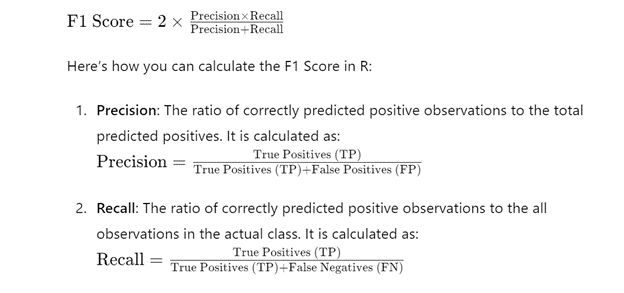
\includegraphics[width=8.67in]{F1score}

\begin{Shaded}
\begin{Highlighting}[]
\NormalTok{tp }\OtherTok{\textless{}{-}}\NormalTok{ conf\_matrix}\SpecialCharTok{$}\NormalTok{result[}\DecValTok{2}\NormalTok{, }\DecValTok{2}\NormalTok{]}
\NormalTok{tn }\OtherTok{\textless{}{-}}\NormalTok{ conf\_matrix}\SpecialCharTok{$}\NormalTok{result[}\DecValTok{1}\NormalTok{, }\DecValTok{1}\NormalTok{]}
\NormalTok{fp }\OtherTok{\textless{}{-}}\NormalTok{ conf\_matrix}\SpecialCharTok{$}\NormalTok{result[}\DecValTok{1}\NormalTok{, }\DecValTok{2}\NormalTok{]}
\NormalTok{fn }\OtherTok{\textless{}{-}}\NormalTok{ conf\_matrix}\SpecialCharTok{$}\NormalTok{result[}\DecValTok{2}\NormalTok{, }\DecValTok{1}\NormalTok{]}

\NormalTok{precision }\OtherTok{\textless{}{-}}\NormalTok{ tp }\SpecialCharTok{/}\NormalTok{ (tp }\SpecialCharTok{+}\NormalTok{ fp) }\CommentTok{\# Calculate precision}
\NormalTok{recall }\OtherTok{\textless{}{-}}\NormalTok{ tp }\SpecialCharTok{/}\NormalTok{ (tp }\SpecialCharTok{+}\NormalTok{ fn) }\CommentTok{\# Calculate recall}
\NormalTok{f1\_score }\OtherTok{\textless{}{-}} \DecValTok{2} \SpecialCharTok{*}\NormalTok{ (precision }\SpecialCharTok{*}\NormalTok{ recall) }\SpecialCharTok{/}\NormalTok{ (precision }\SpecialCharTok{+}\NormalTok{ recall) }\CommentTok{\# Calculate F1 Score}
\FunctionTok{print}\NormalTok{(f1\_score) }\CommentTok{\# Print the F1 Score}
\end{Highlighting}
\end{Shaded}

\begin{verbatim}
[1] 0.9329039
\end{verbatim}

An F1 score of 0.9528796 indicates that your model has a very high level
of precision and recall. This is an excellent score, suggesting that the
model performs well in terms of identifying true positive cases with
very few false positives and false negatives.

\subsubsection{Interpretation:}\label{interpretation}

Precision: The proportion of true positive results among all positive
results predicted by the model. A high precision means that the model
makes few false positive predictions. Recall: The proportion of true
positive results among all actual positive cases. A high recall means
that the model correctly identifies most of the actual positive cases.

\subsection{Strengths and weaknesses of the SVM
algorithm}\label{strengths-and-weaknesses-of-the-svm-algorithm}

While it often isn't easy to tell which algorithms will perform well for
a given task, here are some strengths and weaknesses that will help you
decide whether the SVM algorithm will perform well for your case.

\subsubsection{The strengths of the SVM algorithm are as
follows:}\label{the-strengths-of-the-svm-algorithm-are-as-follows}

\begin{itemize}
\tightlist
\item
  It's very good at learning complex nonlinear decision boundaries.
\item
  It performs very well on a wide variety of tasks.
\item
  It makes no assumptions about the distribution of the predictor
  variables.
\end{itemize}

\subsubsection{The weaknesses of the SVM algorithm are
these:}\label{the-weaknesses-of-the-svm-algorithm-are-these}

\begin{itemize}
\tightlist
\item
  It is one of the most computationally expensive algorithms to train.
\item
  It has multiple hyperparameters that need to be tuned simultaneously.
\item
  It can only handle continuous predictor variables (although recoding a
  categorical variable as numeric may help in some cases).
\end{itemize}

\subsection{Summary}\label{summary-3}

The naive Bayes and support vector machine (SVM) algorithms are
supervised learners for classification problems. Naive Bayes uses Bayes'
rule (defined in chapter 5) to estimate the probability of new data
belonging to each of the possible output classes. The SVM algorithm
finds a hyperplane (a surface with one less dimension than there are
predictors) that best separates the classes. While naive Bayes can
handle both continuous and categorical predictor variables, the SVM
algorithm can only handle continuous predictors. Naive Bayes is
computationally cheap, while the SVM algorithm is one of the most
expensive algorithms. The SVM algorithm can use kernel functions to add
an extra dimension to the data that helps find a linear decision
boundary. The SVM algorithm is sensitive to the values of its
hyperparameters, which must be tuned to maximize performance. The mlr
package allows parallelization of intensive processes, such as
hyperparameter tuning, by using the parallelMap package.

\end{document}
